%\textbf{}%definira klasu dokumenta 
\documentclass[12pt]{report} 

%prostor izmedu naredbi \documentclass i \begin{document} se zove uvod. U njemu se nalaze naredbe koje se odnose na cijeli dokument

%osnovni LaTex ne može riješiti sve probleme, pa se koriste različiti paketi koji olakšavaju izradu željenog dokumenta
\usepackage[croatian]{babel} 
\usepackage{amssymb}
\usepackage{amsmath}
\usepackage{txfonts}
\usepackage{mathdots}
\usepackage{titlesec}
\usepackage{array}
\usepackage{lastpage}
\usepackage{etoolbox}
\usepackage{longtable, tabu}
\usepackage{color, colortbl}
\usepackage[table]{xcolor}
%\usepackage[usenames, dvipsnames]{xcolor}


\usepackage{adjustbox}
\usepackage{geometry}
\usepackage[classicReIm]{kpfonts}
\usepackage{hyperref}
\usepackage{fancyhdr}



\usepackage{float}
\usepackage{setspace}
\restylefloat{table}


\patchcmd{\chapter}{\thispagestyle{plain}}{\thispagestyle{fancy}}{}{} %redefiniranje stila stranice u paketu fancyhdr

%oblik naslova poglavlja
\titleformat{\chapter}{\normalfont\huge\bfseries}{\thechapter.}{20pt}{\Huge}
\titlespacing{\chapter}{0pt}{0pt}{40pt}


\linespread{1.3} %razmak između redaka

\geometry{a4paper, left=1in, top=1in,}  %oblik stranice

\hypersetup{ colorlinks, citecolor=black, filecolor=black, linkcolor=black,	urlcolor=black }   %izgled poveznice


%prored smanjen između redaka u nabrajanjima i popisima
\newenvironment{packed_enum}{
	\begin{enumerate}
		\setlength{\itemsep}{0pt}
		\setlength{\parskip}{0pt}
		\setlength{\parsep}{0pt}
	}{\end{enumerate}}

\newenvironment{packed_item}{
	\begin{itemize}
		\setlength{\itemsep}{0pt}
		\setlength{\parskip}{0pt}
		\setlength{\parsep}{0pt}
	}{\end{itemize}}


%boja za privatni i udaljeni kljuc u tablicama
\definecolor{LightBlue}{rgb}{0.9,0.9,1}
\definecolor{LightGreen}{rgb}{0.9,1,0.9}


%podesavanje zaglavlja i podnožja

\pagestyle{fancy}
\lhead{Programsko inženjerstvo}
\rhead{Papirni.ca}
\lfoot{fooBar}
\cfoot{stranica \thepage/\pageref{LastPage}}
\rfoot{\today}
\renewcommand{\headrulewidth}{0.2pt}
\renewcommand{\footrulewidth}{0.2pt}


\begin{document} 
	
	
	
	\begin{titlepage}
		\begin{center}
			\vspace*{\stretch{1.0}} %u kombinaciji s ostalim \vspace naredbama definira razmak između redaka teksta
			\LARGE Programsko inženjerstvo\\
			\large Ak. god. 2020./2021.\\
			
			\vspace*{\stretch{3.0}}
			
			\huge Papirni.ca\\
			\Large Dokumentacija, Rev. \textit{2}\\
			
			\vspace*{\stretch{12.0}}
			\normalsize
			Grupa: \textit{fooBar}\\
			Voditelj: \textit{Fran Hrabar}\\
			
			
			\vspace*{\stretch{1.0}}
			Datum predaje: \textit{14.1.2021.}\\
	
			\vspace*{\stretch{4.0}}
			
			Nastavnik: \textit{Eugen Vušak}\\
		
		\end{center}

	
	\end{titlepage}

	
	\tableofcontents

	\chapter{Dnevnik promjena dokumentacije}
			
		
		\begin{longtabu} to \textwidth {|X[2, l]|X[13, l]|X[4, l]|X[4, l]|}
			\hline \multicolumn{1}{|l|}{\textbf{Rev.}}	& \multicolumn{1}{l|}{\textbf{Opis promjene/dodatka}} & \multicolumn{1}{|l|}{\textbf{Autori}} & \multicolumn{1}{l|}{\textbf{Datum}} \\[3pt] \hline
			\endfirsthead
			
			\hline \multicolumn{1}{|l|}{\textbf{Rev.}}	& \multicolumn{1}{l|}{\textbf{Opis promjene/dodatka}} & \multicolumn{1}{|l|}{\textbf{Autori}} & \multicolumn{1}{l|}{\textbf{Datum}} \\[3pt] \hline
			\endhead
			
			\hline 
			\endlastfoot
			
			0.1 & Napravljen predložak. \newline Dodan opis zadatka. & Pećanić & 19.10.2020. 		\\[3pt] \hline 
			0.2 & Rad na poglavljima 3 i 4.  & Hrabar & 31.10.2020. 	\\[3pt] \hline  
			0.3 & Rad na poglavljima 3 i 4. \newline Dodani manji detalji u opis.  & Pećanić & 5.11.2020. 	\\[3pt] \hline 
			0.4 & Rad na poglavlju 4. & Hrabar & 7.11.2020. 	\\[3pt] \hline 
			0.5 & Rad na poglavlju \textit{Dodatak}  & Hrabar, Mihovilović, Protulipac, Likakur, Pećanić & 11.11.2020. 	\\[3pt] \hline 
			\textbf{1.0} & Verzija samo s bitnim dijelovima za 1. ciklus & Pećanić, Hrabar & 13.11.2020. \\[3pt] \hline
			1.01 & Promjena manjih tekstualnih detalja u poglavlju 4  & Pećanić & 28.11.2020. 	\\[3pt] \hline 
			1.02 & Promjena dijagrama obrazaca uporabe  & Pećanić & 28.12.2020. 	\\[3pt] \hline 
			1.1 & Rad na poglavlju 5.1 i 6 & Pećanić & 9.1.2021. 	\\[3pt] \hline 
			
			1.2 & Rad na poglavlju 5.4 i 4.1  & Hrabar & 10.1.2021. 	\\[3pt] \hline 
			1.8 & Rad na dijagramu stanja i komponenti  & Vujević & 12.1.2021. 	\\[3pt] \hline 
			1.9 & Rad na poglavljima 4.4, 5.2, 5.3 & Pećanić & 13.1.2021. 	\\[3pt] \hline 
			
			\textbf{2.0} & Konačni tekst predloška dokumentacije  & Hrabar, Mihovilović, Protulipac, Likakur, Pećanić, Vujević, Kukešćak & 14.1.2021. \\[3pt] \hline 
			&  &  & \\[3pt] \hline
			
			
		\end{longtabu}
	
	
	
	\chapter{Opis projektnog zadatka}
		
	
		
		\normalsize{Papirni.ca je aplikacija koja služi za poslovanje prodavaonice papira unutar čije ponude postoje razne vrste i veličine papira uz pojedine dodatne usluge. Usluge variraju ovisno o vrsti korisnika koji se njima služi, a podjela korisnika je sljedeća: }
		
		\begin{packed_enum}
			\item  \textbf{neregistrirani korisnik}
			\item  \textbf{registrirani korisnik}
			
			\begin{packed_enum}
				
				\item privatni
				\item poslovni
				
			\end{packed_enum}
			\item  \textbf{administrator}
			
			
		\end{packed_enum}
	
		\noindent \normalsize{Neregistrirani korisnici mogu mijenjati kontekst platforme iz privatnog u poslovni i obrnuto te im je dostupno isključivo pregledavanje usluga unutar istih, dok je za kupovinu papira i/ili pružanje usluga potrebna registracija.} \\
		
		\noindent \normalsize{Registrirani privatni korisnici za prijavu koriste ime, prezime i e-mail adresu. Jedina usluga koja se pruža ovim korisnicima jest prodaja raznih vrsta papira s obzirom na sljedeće faktore: }
		
		\begin{packed_enum}
			\item \normalsize{boja}
			\item  \normalsize{vrsta}
			\item  \normalsize{težina (gsm)}
			\item  \normalsize{format (A0 - A10)}
		\end{packed_enum}
	
		\noindent \normalsize{Registrirani poslovni korisnici za prijavu koriste ime i OIB firme, ime kontakt osobe iz firme te kontaktni broj telefona i e-mail adresu iste. Kao i privatnima, poslovnim korisnicima omogućena je prodaja papira koja, uz već navedene, ima dvije dodatne opcije - izbor nekonvencionalne veličine papira po narudžbi i mogućnost dodatka vodenog žiga na papire. Korisnik mora priložiti sliku koju želi upotrijebiti kao vodeni žig ako odabere tu opciju. Osim prodaje papira, poslovnim korisnicima je omogućeno slanje posebnog tekstualnog zahtjeva putem kojeg se može zatražiti usluga koja nije u standardnoj ponudi papirnice - npr. specifičan način pakiranja narudžbe. Da bi dodatni zahtjev bio validan, korisnik mora unijeti kratki naziv usluge koju traži i kontakt podatke. Uz jednokratno korištenje usluga, poslovni korisnici mogu napraviti mjesečnu pretplatu na neki proizvod - time se odabrana kupovina obavlja automatski svaki mjesec. Ako korisnik u košarici ima proizvode koje kupuje jednokratno uz one koji su označeni za pretplatu, nakon potvrde kupnje svi će proizvodi biti naplaćeni s time da će se oni označeni za pretplatu naplaćivati mjesečno od tog trenutka do otkazivanja pretplate. Poslovni korisnik može pregledavati svoje pretplate i otkazati ih u bilo kojem trenutku.} \\
		
		\noindent \normalsize{Administratorima je omogućeno sljedeće: } 
		\begin{packed_enum}
			\item \normalsize{pregled povijesti kupljenih usluga za sve korisnike}
			\item  \normalsize{pregled i otkazivanje pretplata poslovnih korisnika}
			\item  \normalsize{pregled i mogućnost uklanjanja dodatnih uskuga dodanih putem tekstualnog zahtjeva} \\
		\end{packed_enum}
	
		\noindent \normalsize{Kupovina funkcionira na sljedeći način: odabirom na proizvod on se dodaje u košaricu, a plaćanje se vrši putem servisa PayPal. Dodatna usluga slanja tekstualnog zahtjeva se ne dodaje u košaricu nego se za nju napisani zahtjev najprije mora odobriti i tek kada (i ako) je on odobren zahtjev će se dodati tom poslovnom korisniku. U slučaju problema sa zahtjevom, korisnika se obavještava putem kontakt podataka koji su uneseni prilikom predaje zahtjeva te se istim putem i rješavaju. Nakon rješavanja potencijalnih problema dodatna usluga se dodaje korisniku, a njega se obavještava o uspješnom dodavanju usluge (također putem prethodno navedenih kontakt podataka). Takva usluga vidljiva je isključivo tom korisniku (među ostalim uslugama). } \\
		
		
		\noindent \normalsize{Projekt kao što je Papirni.ca  može koristiti bilo kojem manjem obrtu koji se bavi ovakvom djelatnošću, a uz proširenje bi se ovakva aplikacija mogla koristiti i za veće trgovine. Budući da se zbog pandemije koronavirusa naglašava smanjenje međuljudskog kontakta na minimum, online trgovine postaju sve prometnije tako da bi ovakvo rješenje bilo iznimno prikladno za papirnice koje posluju u ovo doba. Izuzevši trenutnu situaciju, ovakav pristup pogodan je udaljenim kupcima koji nisu u mogućnosti fizički posjetiti trgovinu i osobno napraviti narudžbu. Također, kupovina putem aplikacije ima određenu preglednost s izlistanim opcijama  koju kupci možda ne bi dobili jednim pogledom u fizičkoj papirnici.} 
		
		\noindent \normalsize{Primjer sličan ovome projektu je web-stranica  knjižare i papirnice Denova (\url{https://www.denova.hr/}). Njihova ponuda nije ograničena samo na papire, no kao i kod Papirni.ca aplikacije, među papirima također postoji mnogo opcija i dosta širok izbor.} \\
		
	
		%\noindent \underbar{podcrtani tekst}, \textbf{podebljani tekst}, 	%\textit{nagnuti tekst}\\
		%\noindent \normalsize primjer \large primjer \Large primjer \LARGE %{primjer} \huge {primjer} \Huge primjer \normalsize
	
		%\noindent primjer url-a: %\url{https://www.fer.unizg.hr/predmet/proinz/projekt}
		
		%\noindent posebni znakovi: \# \$ \% \& \{ \} \_ 
	%	$|$ $<$ $>$ 
	%	\^{} 
	%	\~{} 
	%	$\backslash$ 
		 %
		 %\begin{packed_item}
		 	%\item \textit{tocka}
		 	
		 %\end{packed_item}
	
		%unos slike
		\begin{figure}[H]
			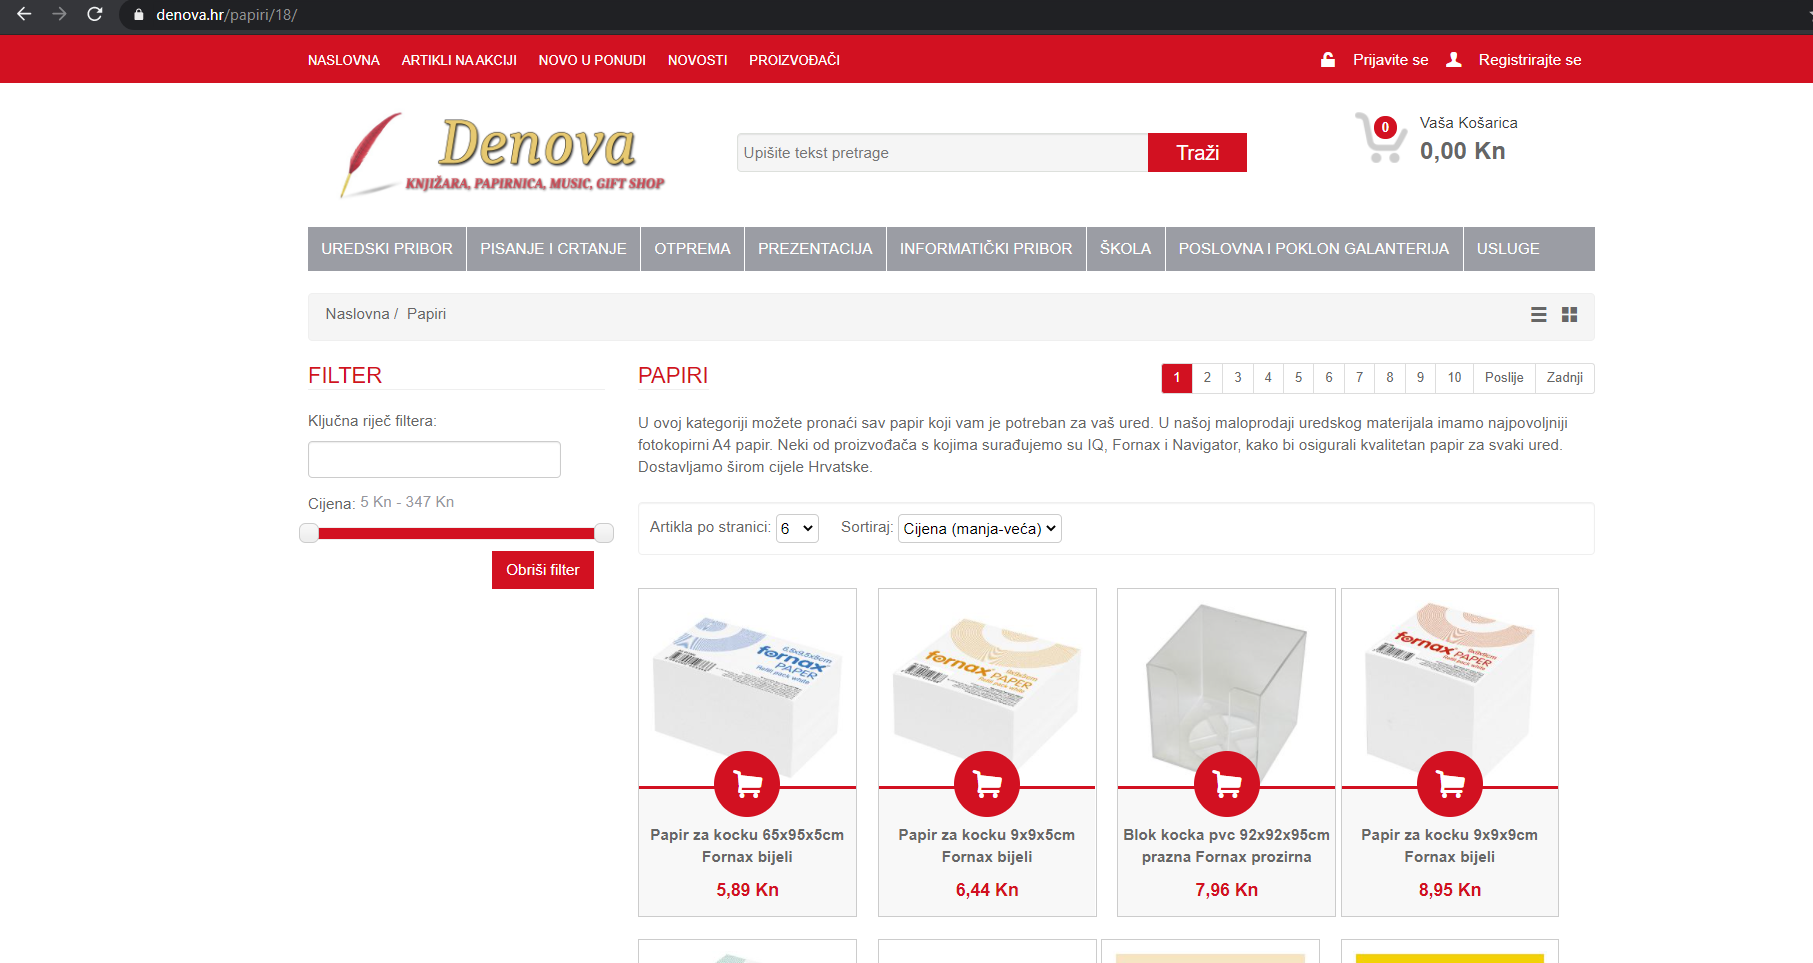
\includegraphics[scale=0.3]{slike/denova1.PNG} %veličina slike u odnosu na originalnu datoteku i pozicija slike
			
			%	\includegraphics[width=.9\linewidth]{slike/aktivnost.PNG} %veličina u odnosu na širinu linije
			\centering
			\caption{Snimka web-stranice papirnice Denova}
			\label{fig:denova1}%label mora biti drugaciji za svaku sliku
		\end{figure}
			%Referenciranje slike \ref{fig:denova1} u tekstu.
		\noindent \normalsize{   } \\
		\begin{figure}[H]
			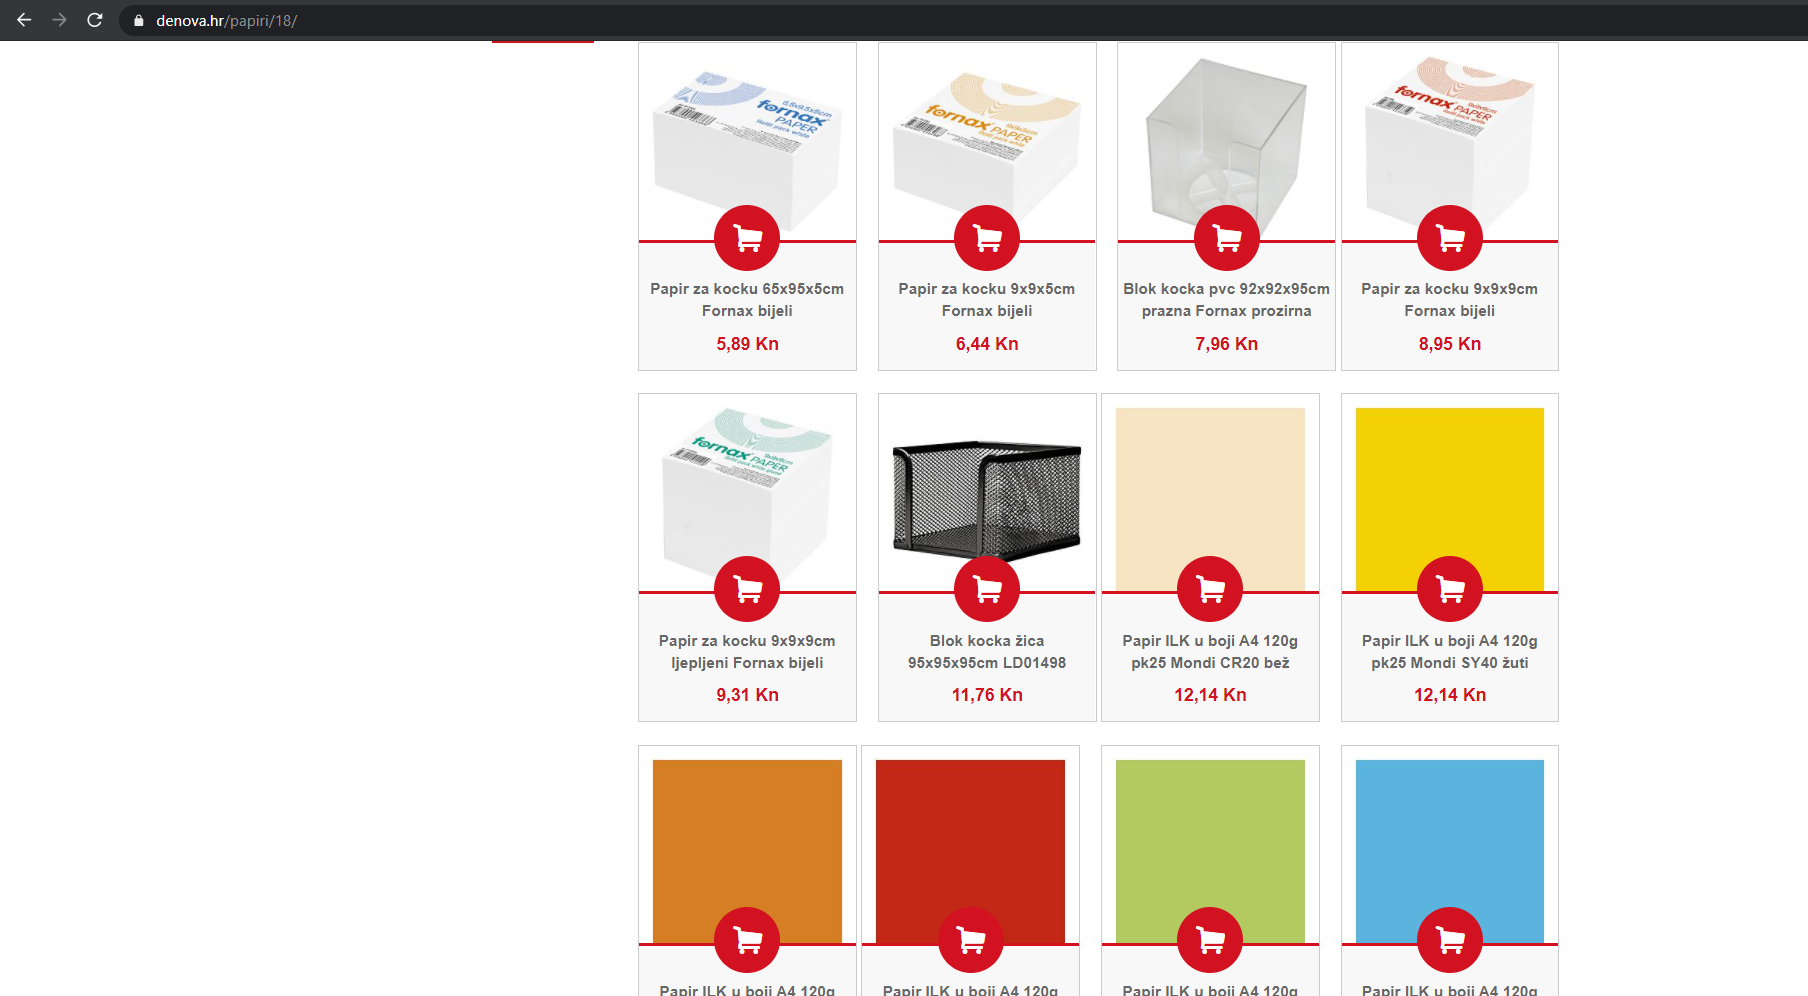
\includegraphics[scale=0.3]{slike/denova2.PNG} %veličina slike u odnosu na originalnu datoteku i pozicija slike
			
			%	\includegraphics[width=.9\linewidth]{slike/aktivnost.PNG} %veličina u odnosu na širinu linije
			\centering
			\caption{Snimka raznolike ponude papira papirnice Denova} 
			\label{fig:denova2}%label mora biti drugaciji za svaku sliku
		\end{figure}
		
		\noindent \normalsize{Papirni.ca namijenjena je svakome tko ima interes kupovati papir putem aplikacije. Za pretpostaviti je da bi se njome među privatnim korisnicima našlo dosta studenata i učenika budući da su mladi skloniji ovakvoj vrsti kupovine jer su tehnički pismeniji od starijih generacija. Dodatne usluge koje se pružaju poslovnim korisnicima zasigurno bi bile primamljive obrtnicima i manjim firmama koje koriste svoj logo na papirima koji su priloženi uz isporuku proizvoda. } \\
		
		\noindent \normalsize{Projektno rješenje moglo bi se prilagoditi na više načina. Proširenjem ponude proizvoda mogla bi se ostvariti aplikacija za rad knjižare ili kakve veće trgovine sa sličnim asortimanom. Međutim, samo promjenom vrste proizvoda i opcija koje se za njih mogu odabrati, ovakva aplikacija mogla bi se koristiti za razne trgovine i obrte kao što su slastičarnica, pekara, trgovina odjećom, trgovina igračkama i sl.} \\
		
		\noindent \normalsize{Projekt Papirni.ca od resursa ima na raspolaganju (ljudsku) radnu snagu članova tima fooBar, (besplatan) pristup mnogim razvojnim okruženjima i vrstama programske potpore zahvaljujući FER-u te vremenski okvir od 1.10.2020. do 14.1.2021. za isporuku. Finalna isporuka projekta jest aplikacija modernog i vizualno privlačnog dizajna koja sadrži funkcionalnosti navedene ranije u ovom poglavlju, no prije finalne isporuke postoji nekoliko kontrolnih točaka koje obuhvaćaju isporuku aplikacije u verziji koja je dotad napravljena. Rokovi vezani uz periodične (djelomične) isporuke aplikacije dani su u sljedećoj tablici:} \\
		
		\begin{center}
			\begin{tabular}{ |c|c| } 
				\hline
				\textbf {Rok}& \textbf{Opis isporuke}  \\
				\hline
				13.11.2020. & Predaja projekta za prvi ciklus (v0.0)  \\
				\hline
				7.1.-13.1.2021. & Demonstracija alfa inačice rada  aplikacije  \\
				\hline
				14.1.2021. & Predaja projekta za drugi ciklus (finalna isporuka)  \\
				\hline
				
				
				\hline
			\end{tabular}
		\end{center}
		
		\noindent \normalsize{\\}
		
		\noindent \normalsize{Mogućih nadogradnji ovakvog rješenja ima mnogo. Neke od njih su: dodavanje teksture papira kao još jedne opcije pri kupnji papira, omogućavanje neregistriranim korisnicima da bez registracije (uz jednokratno davanje svojih podataka) naprave narudžbu, dodavanje godišnjih pretplata za poslovne korisnike.} \\
		
	
		
		\eject
		
	
	\chapter{Specifikacija programske potpore}
		
	\section{Funkcionalni zahtjevi}
			
			%\textbf{\textit{dio 1. revizije}}\\
			
			%\textit{Navesti \textbf{dionike} koji imaju \textbf{interes u ovom sustavu} ili  \textbf{su nositelji odgovornosti}. To su prije svega korisnici, ali i administratori sustava, naručitelji, razvojni tim.}\\
				
		%	\textit{Navesti \textbf{aktore} koji izravno \textbf{koriste} ili \textbf{komuniciraju sa sustavom}. Oni mogu imati inicijatorsku ulogu, tj. započinju određene procese u sustavu ili samo sudioničku ulogu, tj. obavljaju određeni posao. Za svakog aktora navesti funkcionalne zahtjeve koji se na njega odnose.}\\
			
			
			\noindent \textbf{Dionici:}
			
			\begin{packed_enum}
				
				\item Vlasnik (naručitelj)
				\item Klijenti
				\begin{packed_enum}
					\item Privatni
					\item Poslovni
				\end{packed_enum}				
				\item Administrator
				\item Razvojni tim
				
			\end{packed_enum}
			
			\noindent \textbf{Aktori i njihovi funkcionalni zahtjevi:}
			
			
			\begin{packed_enum}
				\item  \underbar{Neregistrirani/neprijavljeni korisnik (inicijator) može:}
				
				\begin{packed_enum}
					
					\item jednostavno mijenjati  kontekst  iz  privatnog  u  poslovni  i  obrnuto
					\item pregledavati predefinirane izbore boja, vrsta, težina i formata papira
				%	\begin{packed_enum}
						
					%	\item  podfunkcionalnost 1 
					%	\item  podfunkcionalnost 2
				
				%	\end{packed_enum}
				%	\item  funkcionalnost 3
					
				\end{packed_enum}
			
				\item  \underbar{Privatni klijent (inicijator) može:}
				
				\begin{packed_enum}
					
					\item odabrati predefinirane izbore boja, vrsta, težina i formata papira i platiti svoju narudžbu
					
				\end{packed_enum}
			
				\item  \underbar{Poslovni klijent (inicijator) može:}
				
				\begin{packed_enum}
					
					\item odabrati predefinirane izbore boja, vrsta, težina i formata papira i platiti svoju narudžbu
					
					\item odabrati papir nekonvencionalnih veličina i dodati vodeni žig
					
					\item zatražiti dodatne usluge koje nisu na ponudi
					
					\item  pregledavati i odabrati potvrđene dodatne usluge
					
					\item zakazati, pregledavati i otkazivati mjesečne pretplate
					
				\end{packed_enum}
			
				\item  \underbar{Administrator (inicijator) može:}
				
				\begin{packed_enum}
					
					\item pregledavanti pojedine tekstualne zahtjeve poslovnih klijenata, te potvrditi ili odbiti i uklanjati iste
					
					\item pregledavati i otkazivati mjesečne pretplate
					
					\item pregledavati povijest kupljenih usluga za  sve  korisnike
					
				\end{packed_enum}
				
				\item  \underbar{Baza podataka (sudionik) može:}
				
				\begin{packed_enum}
					
					\item pohranjivati podatke o klijentima
					\item pohranjivati podatke o artiklima na ponudi
					\item pohranjivati narudžbe
					
				\end{packed_enum}
			\end{packed_enum}
			
			\eject 
			
			
				
			\subsection{Obrasci uporabe}
				
				%\textbf{\textit{dio 1. revizije}}
				
				%\subsubsection{Opis obrazaca uporabe}
					%\textit{Funkcionalne zahtjeve razraditi u obliku obrazaca uporabe. Svaki obrazac je potrebno razraditi prema donjem predlošku. Ukoliko u nekom koraku može doći do odstupanja, potrebno je to odstupanje opisati i po mogućnosti ponuditi rješenje kojim bi se tijek obrasca vratio na osnovni tijek.}\\
					

					\noindent \underbar{\textbf{UC1-Pregled preddefiniranih papira}}
					\begin{packed_item}
	
						\item \textbf{Glavni sudionik: } Korisnik, klijent
						\item  \textbf{Cilj:} Pregledavanje preddefiniranih artikala
						\item  \textbf{Sudionici:} Baza podataka
						\item  \textbf{Preduvjet:} -
						\item  \textbf{Opis osnovnog tijeka:}
						
						\item[] \begin{packed_enum}
	
							\item Korisnik odabire opciju za pregled papira u načinu za privatnog klijenta
							\item Korisnik pregledava postojeće opcije po padajućim izbornicima
						\end{packed_enum}
					
					\end{packed_item}
				
			
					\noindent \underbar{\textbf{UC2-Registracija privatnog klijenta}}
					\begin{packed_item}
						
						\item \textbf{Glavni sudionik: } Korisnik
						\item  \textbf{Cilj:} Stvoriti privatni korisnički račun
						\item  \textbf{Sudionici:} Baza podataka
						\item  \textbf{Preduvjet:} -
						\item  \textbf{Opis osnovnog tijeka:}
						
						\item[] \begin{packed_enum}
							
							\item Korisnik odabire opciju za registraciju privatnog klijenta
							\item Korisnik unosi potrebne korisničke podatke
							\item Korisnik prima obavijest o uspješnoj registraciji
						\end{packed_enum}
						
						\item  \textbf{Opis mogućih odstupanja:}
						
						\item[] \begin{packed_item}
							
							\item[2.a]  Odabir već zauzetog korisničkog imena i/ili e-maila, unos korisničkog podatka u nedozvoljenom formatu ili pružanje neispravnoga e-maila
							\item[] \begin{packed_enum}
								
								\item Sustav obavještava korisnika o neuspjelom upisu i vraća ga na stranicu za registraciju
								\item  Korisnik mijenja potrebne podatke te završava unos ili odustaje od registracije
								
							\end{packed_enum}
						\end{packed_item}
					\end{packed_item}
				
					\noindent \underbar{\textbf{UC3-Registracija poslovnog klijenta}}
					\begin{packed_item}
						
						\item \textbf{Glavni sudionik: } Korisnik
						\item  \textbf{Cilj:} Stvoriti poslovni korisnički račun
						\item  \textbf{Sudionici:} Baza podataka
						\item  \textbf{Preduvjet:} -
						\item  \textbf{Opis osnovnog tijeka:}
						
						\item[] \begin{packed_enum}
							
							\item Korisnik odabire opciju za registraciju poslovnog klijenta
							\item Korisnik unosi potrebne korisničke podatke
							\item Korisnik prima obavijest o uspješnoj registraciji
						\end{packed_enum}
						
						\item  \textbf{Opis mogućih odstupanja:}
						
						\item[] \begin{packed_item}
							
							\item[2.a]  Odabir već zauzetog ili neispravnog imena kompanije, OIB-a, kontakt osobe, telefona i/ili e-maila
							\item[] \begin{packed_enum}
								
								\item Sustav obavještava korisnika o neuspjelom upisu i vraća ga na stranicu za registraciju
								\item  Korisnik mijenja potrebne podatke te završava unos ili odustaje od registracije
								
							\end{packed_enum}
						\end{packed_item}
					\end{packed_item}
				
					\noindent \underbar{\textbf{UC4-Prijava privatnog klijenta u sustav}}
					\begin{packed_item}
						
						\item \textbf{Glavni sudionik: } Privatni klijent
						\item  \textbf{Cilj:} Dobiti pristup korisničkom sučelju
						\item  \textbf{Sudionici:} Baza podataka
						\item  \textbf{Preduvjet:} Registracija
						\item  \textbf{Opis osnovnog tijeka:}
						
						\item[] \begin{packed_enum}
							
							\item Korisnik odabire opciju za registraciju privatnog klijenta
							\item Korisnik unosi potrebne korisničke podatke
							\item Korisnik prima obavijest o uspješnoj prijavi
							\item Korisnik gubi pristup poslovnim funkcijama
						\end{packed_enum}
						
						\item  \textbf{Opis mogućih odstupanja:}
						
						\item[] \begin{packed_item}
							
							\item[2.a]  Neispravno ime i/ili lozinka
							\item[] \begin{packed_enum}
								
								\item Sustav obavještava korisnika o neuspjelom upisu i vraća ga na stranicu za prijavu
								\item Korisnik ponovno unosi podatke za prijavu ili odustaje od prijave
							
							\end{packed_enum}
						\end{packed_item}
					\end{packed_item}
				
					\noindent \underbar{\textbf{UC5-Prijava poslovnog klijenta u sustav}}
					\begin{packed_item}
						
						\item \textbf{Glavni sudionik: } Poslovni klijent
						\item  \textbf{Cilj:} Dobiti pristup korisničkom sučelju
						\item  \textbf{Sudionici:} Baza podataka
						\item  \textbf{Preduvjet:} Registracija
						\item  \textbf{Opis osnovnog tijeka:}
						
						\item[] \begin{packed_enum}
							
							\item Korisnik odabire opciju za registraciju poslovnog klijenta
							\item Korisnik unosi potrebne korisničke podatke
							\item Korisnik prima obavijest o uspješnoj prijavi
						\end{packed_enum}
						
						\item  \textbf{Opis mogućih odstupanja:}
						
						\item[] \begin{packed_item}
							
							\item[2.a]  Neispravno ime i/ili lozinka
							\item[] \begin{packed_enum}
								
								\item Sustav obavještava korisnika o neuspjelom upisu i vraća ga na stranicu za prijavu
								\item Korisnik ponovno unosi podatke za prijavu ili odustaje od prijave
								
							\end{packed_enum}
						\end{packed_item}
					\end{packed_item}
				
					\noindent \underbar{\textbf{UC6-Dodavanje usluge u košaricu}}
					\begin{packed_item}
						
						\item \textbf{Glavni sudionik: } Klijent
						\item  \textbf{Cilj:} Dodati uslugu u košaricu
						\item  \textbf{Sudionici:} -
						\item  \textbf{Preduvjet:} Korisnik je prijavljen
						\item  \textbf{Opis osnovnog tijeka:}
						
						\item[] \begin{packed_enum}
							
							\item Klijent odabire preddefiniranu uslugu
							\item Klijent odabire opciju "Dodaj u košaricu"
						\end{packed_enum}
					
						\item  \textbf{Opis mogućih odstupanja:}
						
						\item[] \begin{packed_item}
							
							\item[2.a]  Nisu odabrani svi podaci o papiru
							\item[] \begin{packed_enum}
								
								\item Sustav obavještava klijenta o neuspjelom odabiru i pita ga da provjeri podatke
								\item  Klijent odabire potrebne podatke te odabire opciju "Dodaj u košaricu" ili odustaje od dodavanja
							\end{packed_enum}
						\end{packed_item}
					\end{packed_item}
				
					\noindent \underbar{\textbf{UC7-Dodavanje papira posebne dimenzije i/ili sa žigom u košaricu}}
					\begin{packed_item}
						
						\item \textbf{Glavni sudionik: } Poslovni klijent
						\item  \textbf{Cilj:} Dodati papira posebne dimenzije i/ili sa žigom u košaricu
						\item  \textbf{Sudionici:} -
						\item  \textbf{Preduvjet:} Korisnik je prijavljen
						\item  \textbf{Opis osnovnog tijeka:}
						
						\item[] \begin{packed_enum}
							
							\item Klijent odabire dimenzije papira i/ili priloži sliku vodenog žiga
							\item Klijent odabire opciju "Dodaj u košaricu"
						\end{packed_enum}
						
						\item  \textbf{Opis mogućih odstupanja:}
						
						\item[] \begin{packed_item}
							
							\item[2.a]  Dimenzije izvan određenih granica ili u krivom formatu
							\item[] \begin{packed_enum}
								
								\item Sustav obavještava klijenta o neuspjelom upisu i pita ga da provjeri podatke
								\item  Klijent mijenja potrebne podatke te odabire opciju "Dodaj u košaricu" ili odustaje od dodavanja
								
							\end{packed_enum}
						
							\item[2.b]  Vodeni žig u krivom formatu
							\item[] \begin{packed_enum}
								\item Sustav obavještava klijenta o neuspjelom prilogu žiga i obavještava ga da je potrebna slika žiga
								\item klijent prilaže sliku te odabire opciju "Dodaj u košaricu" ili odustaje od dodavanja
						\end{packed_enum}
					\end{packed_item}
				\end{packed_item}
				
				\noindent \underbar{\textbf{UC8-Slanje tekstualnog zahtjeva za dodatne usluge}}
				\begin{packed_item}
					
					\item \textbf{Glavni sudionik: } Poslovni klijent
					\item  \textbf{Cilj:}  Zatražiti uslugu koja nije na ponudi
					\item  \textbf{Sudionici:} Baza podataka, administrator
					\item  \textbf{Preduvjet:} Korisnik je prijavljen
					\item  \textbf{Opis osnovnog tijeka:}
					
					\item[] \begin{packed_enum}
						
						\item Klijent odabire opciju za slanje tekstualnog zahtjeva
						\item Klijent unosi zahtjev, naziv usluge i kontakt podatke
						\item Klijent prima obavijest da njegov zahtjev čeka potvrdu
					
					\end{packed_enum}
					
					\item  \textbf{Opis mogućih odstupanja:}
					
					\item[] \begin{packed_item}
						
						\item[2.a]  Unesen zahtjev i opis su prazni
						\item[] \begin{packed_enum}
							
							\item Sustav obavještava klijenta da zahtjevi ne mogu biti prazni
							\item  Klijent unosi potrebne podatke te završava unos ili odustaje od zahtjeva
							
						\end{packed_enum}
					
						\item[2.b]  Uneseni neispravni kontakt podaci
						\item[] \begin{packed_enum}
							
							\item Sustav obavještava klijenta o neispravnosti kontakt podataka
							\item  Klijent mijenja kontakt podatke te završava unos ili odustaje od registracije
							
						\end{packed_enum}
					\end{packed_item}
				\end{packed_item}
			
				\noindent \underbar{\textbf{UC9-Zakazivanje mjesečne pretplate}}
				\begin{packed_item}
					
					\item \textbf{Glavni sudionik: } Poslovni klijent
					\item  \textbf{Cilj:} Zakazivanje mjesečne pretplate za pojedine usluge
					\item  \textbf{Sudionici:} Baza podataka
					\item  \textbf{Preduvjet:} Korisnik je prijavljen
					\item  \textbf{Opis osnovnog tijeka:}
					
					\item[] \begin{packed_enum}
						
						\item Klijent odabire svoju košaricu
						\item Klijent u košarici odabire usluge za koje želi mjesečnu pretplatu i označava ih
					
					\end{packed_enum}
					
				\end{packed_item}
			
				\noindent \underbar{\textbf{UC10-Pregled mjesečnih pretplata}}
				\begin{packed_item}
					
					\item \textbf{Glavni sudionik: } Poslovni klijent
					\item  \textbf{Cilj:} Pregledavanje aktivnih mjesečnih pretplata
					\item  \textbf{Sudionici:} Baza podataka
					\item  \textbf{Preduvjet:} Korisnik je prijavljen
					\item  \textbf{Opis osnovnog tijeka:}
					
					\item[] \begin{packed_enum}
						
						\item Klijent odabire opciju za pregled mjesečnih pretplata
						
					\end{packed_enum}
					
				\end{packed_item}
			
				\noindent \underbar{\textbf{UC11-Otkazivanje mjesečnih pretplata}}
				\begin{packed_item}
					
					\item \textbf{Glavni sudionik: } Poslovni klijent
					\item  \textbf{Cilj:} Otkazivanje mjesečnih pretplata
					\item  \textbf{Sudionici:} Baza podataka, administrator
					\item  \textbf{Preduvjet:} Korisnik je prijavljen i postoje mjesečne pretplate
					\item  \textbf{Opis osnovnog tijeka:}
					
					\item[] \begin{packed_enum}
						
						\item Klijent odabire opciju za pregled mjesečnih pretplata
						\item Klijent odabire mjesečnu pretplatu koju želi otkazati
						\item Klijent prima obavijest da je pretplata otkazana
						
					\end{packed_enum}
					
				\end{packed_item}
			
				\noindent \underbar{\textbf{UC12-Pregled sadržaja košarice}}
				\begin{packed_item}
					
					\item \textbf{Glavni sudionik: } Klijent
					\item  \textbf{Cilj:} Prikaz i pregled sadržaja košarice
					\item  \textbf{Sudionici:} -
					\item  \textbf{Preduvjet:} Korisnik je prijavljen
					\item  \textbf{Opis osnovnog tijeka:}
					
					\item[] \begin{packed_enum}
						
						\item Klijent odabire opciju za pregled košarice
						
					\end{packed_enum}
					
				\end{packed_item}
			
				\noindent \underbar{\textbf{UC13-Uređivanje sadržaja košarice}}
				\begin{packed_item}
					
					\item \textbf{Glavni sudionik: } Klijent
					\item  \textbf{Cilj:} Micanje usluga iz košarice, promjena kvantitete
					\item  \textbf{Sudionici:} -
					\item  \textbf{Preduvjet:} Korisnik je prijavljen
					\item  \textbf{Opis osnovnog tijeka:}
					
					\item[] \begin{packed_enum}
						
						\item Klijent odabire opciju za pregled košarice
						\item Klijent makne i/ili uređuje usluge u košarici
						
					\end{packed_enum}
				
				\end{packed_item}
			
				\noindent \underbar{\textbf{UC14-Naručivanje usluga}}
				\begin{packed_item}
					
					\item \textbf{Glavni sudionik: } Klijent
					\item  \textbf{Cilj:} Potvrditi narudžbu kako bi ju mogao platiti
					\item  \textbf{Sudionici:} -
					\item  \textbf{Preduvjet:} Korisnik je prijavljen
					\item  \textbf{Opis osnovnog tijeka:}
					
					\item[] \begin{packed_enum}
						
						\item Klijent odabire opciju za pregled košarice
						\item Klijent odabire opciju za naručivanje
						\item Klijent se usmjeri na plaćanje usluge
						
					\end{packed_enum}
					
					\item  \textbf{Opis mogućih odstupanja:}
					
					\item[] \begin{packed_item}
						
						\item[2.a] Košarica je prazna
						\item[] \begin{packed_enum}
							
							\item Klijenta sustav obavijesti da se narudžba provodi samo nad nepraznom košaricom i vraća ga se na pregled košarice
							
						\end{packed_enum}
						
					\end{packed_item}
				\end{packed_item}
			
				\noindent \underbar{\textbf{UC15-Plaćanje usluge}}
				\begin{packed_item}
					
					\item \textbf{Glavni sudionik: } Klijent
					\item  \textbf{Cilj:} Plaćanje usluge kako bi proces kupnje usluge bio završen
					\item  \textbf{Sudionici:} Baza podataka
					\item  \textbf{Preduvjet:} Korisnik je prijavljen
					\item  \textbf{Opis osnovnog tijeka:}
					
					\item[] \begin{packed_enum}
						
						\item Klijent za odabranu opciju plaćanja unosi svoje podatke
						\item Klijent potvrđuje plaćanje
						\item Košarica se isprazni i klijenta se vraća na pregled košarice
					\end{packed_enum}
					
					\item  \textbf{Opis mogućih odstupanja:}
					
					\item[] \begin{packed_item}
						
						\item[2.a] Nedovoljan iznos na računu za plaćanje narudžbe
						\item[] \begin{packed_enum}
							
							\item Klijenta se obavještava da je iznos nedostatan za plaćanje narudžbe i vraća ga na pregled košarice
							
						\end{packed_enum}
						
					\end{packed_item}
				\end{packed_item}
			
				\noindent \underbar{\textbf{UC16-Prikaz povijesti kupljenih usluga za sve korisnike}}
				\begin{packed_item}
					
					\item \textbf{Glavni sudionik: } Administrator
					\item  \textbf{Cilj:} Prikaz povijesti kupljenih usluga za sve korisnike
					\item  \textbf{Sudionici:} Baza podataka
					\item  \textbf{Preduvjet:} Korisnik je prijavljen
					\item  \textbf{Opis osnovnog tijeka:}
					
					\item[] \begin{packed_enum}
						
						\item Administrator odabire opciju za prikaz povijesti kupljenih usluga
					\end{packed_enum}
					
				\end{packed_item}

				\noindent \underbar{\textbf{UC17-Prikaz vlastite povijesti kupljenih usluga}}
				\begin{packed_item}
					
					\item \textbf{Glavni sudionik: } Klijent
					\item  \textbf{Cilj:} Prikaz vlastite povijesti kupljenih usluga
					\item  \textbf{Sudionici:} Baza podataka
					\item  \textbf{Preduvjet:} Korisnik je prijavljen
					\item  \textbf{Opis osnovnog tijeka:}
					
					\item[] \begin{packed_enum}
						
						\item Klijent odabire opciju za prikaz povijesti kupljenih usluga
						
					\end{packed_enum}
				\end{packed_item}
			
				\noindent \underbar{\textbf{UC18-Potvrđivanje dodatnih usluga}}
				\begin{packed_item}
					
					\item \textbf{Glavni sudionik: } Administrator, poslovni klijent
					\item  \textbf{Cilj:} Potvrđivanje i dodavanje dodatnih usluga, poslanih tekstualnim zahtjevom, poslovnom klijentu
					\item  \textbf{Sudionici:} Baza podataka
					\item  \textbf{Preduvjet:} Administrator je prijavljen i tekstualni zahtjev postoji
					\item  \textbf{Opis osnovnog tijeka:}
					
					\item[] \begin{packed_enum}
						
						\item Administrator odabire opciju za prikaz tekstualnih zahtjeva koji čekaju potvrdu
						\item Administrator odabire zahtjev koji želi potvrditi i potvrđuje ga
						\item Zahtjev se makne iz administratorovog prikaza tekstualnih zahtjeva koji čekaju potvrdu i prikazuje u opciji dodatnih usluga poslovnog klijenta čiji je zahtjev potvrđen
						
					\end{packed_enum}
					
				%	\item  \textbf{Opis mogućih odstupanja:}
					
				%	\item[] \begin{packed_item}
						
					%	\item[2.a] $<$opis mogućeg scenarija odstupanja u koraku 2$>$
					%	\item[] \begin{packed_enum}
							
						%	\item $<$opis rješenja mogućeg scenarija korak 1$>$
						%	\item $<$opis rješenja mogućeg scenarija korak 2$>$
							
						%\end{packed_enum}
						%\item[2.b] $<$opis mogućeg scenarija odstupanja u koraku 2$>$
					%	\item[3.a] $<$opis mogućeg scenarija odstupanja  u koraku 3$>$
						
				%	\end{packed_item}
				\end{packed_item}
			
				\noindent \underbar{\textbf{UC19-Odbijanje dodatnih usluga}}
				\begin{packed_item}
					
					\item \textbf{Glavni sudionik: } Administrator, poslovni klijent
					\item  \textbf{Cilj:} Odbijanje dodatnih usluga, poslanih tekstualnim zahtjevom, poslovnom klijentu
					\item  \textbf{Sudionici:} Baza podataka
					\item  \textbf{Preduvjet:} Administrator je prijavljen i tekstualni zahtjev postoji
					\item  \textbf{Opis osnovnog tijeka:}
					
					\item[] \begin{packed_enum}
						
						\item Administrator odabire opciju za prikaz tekstualnih zahtjeva koji čekaju potvrdu
						\item Administrator odabire zahtjev koji želi odbiti i odbija ga
						\item Zahtjev se makne iz administratorovog prikaza tekstualnih zahtjeva koji čekaju potvrdu i obavještava se poslovnog klijenta kojem je zahtjev odbijen
						
					\end{packed_enum}
				\end{packed_item}
			
			
				\noindent \underbar{\textbf{UC20-Pregled potvrđenih dodatnih usluga}}
				\begin{packed_item}
					
					\item \textbf{Glavni sudionik: } Administrator
					\item  \textbf{Cilj:} Pregledavanje potvrđenih  dodatnih usluga
					\item  \textbf{Sudionici:} Baza podataka
					\item  \textbf{Preduvjet:} Administrator je prijavljen
					\item  \textbf{Opis osnovnog tijeka:}
					
					\item[] \begin{packed_enum}
						
						\item Administrator odabire opciju za pregled potvrđenih dodatnih usluga
						\item Administrator pregledava sve potvrđene dodatne usluge
						
					\end{packed_enum}
				\end{packed_item}
			
				
			
				\noindent \underbar{\textbf{UC21-Uklanjanje potvrđenih dodatnih usluga}}
				\begin{packed_item}
					
					\item \textbf{Glavni sudionik: } Administrator, poslovni klijent
					\item  \textbf{Cilj:} Uklanjanje potvrđenih dodatnih usluga iz ponude poslovnog klijenta
					\item  \textbf{Sudionici:} Baza podataka
					\item  \textbf{Preduvjet:} Administrator je prijavljen i potvrđene dodatne usluge postoje
					\item  \textbf{Opis osnovnog tijeka:}
					
					\item[] \begin{packed_enum}
						
						\item Administrator odabire opciju za prikaz potvrđenih dodatnih usluga
						\item Administrator odabire zahtjev koji želi ukloniti i uklanja ga
						\item Zahtjev se makne iz administratorovog prikaza potvrđenih dodatnih usluga, obavještava se poslovnog klijenta i uklanja mu se dodatna usluga kao i postojeće pretplate sa tom uslugom
						
					\end{packed_enum}
				\end{packed_item}
			
				\noindent \underbar{\textbf{UC22-Pregled dodatnih usluga}}
				\begin{packed_item}
					
					\item \textbf{Glavni sudionik: } Poslovni klijent
					\item  \textbf{Cilj:} Pregled dodatnih usluga ovog poslovnog klijenta
					\item  \textbf{Sudionici:} Baza podataka
					\item  \textbf{Preduvjet:} Korisnik je prijavljen
					\item  \textbf{Opis osnovnog tijeka:}
					
					\item[] \begin{packed_enum}
						
						\item Klijent odabire opciju za prikaz dodatnih usluga
						
					\end{packed_enum}
				\end{packed_item}

				\noindent \underbar{\textbf{UC23-Dodavanje dodatnih usluga u košaricu}}
				\begin{packed_item}
					
					\item \textbf{Glavni sudionik: } Poslovni klijent
					\item  \textbf{Cilj:} Dodavanje dodatnih usluga u košaricu
					\item  \textbf{Sudionici:} -
					\item  \textbf{Preduvjet:} Klijent je prijavljen
					\item  \textbf{Opis osnovnog tijeka:}
					
					\item[] \begin{packed_enum}
						
						\item Klijent odabire dodatnu uslugu među potvrđenim dodatnim uslugama i dodaje ju u košaricu 
						
						
					\end{packed_enum}
				
					
				
				
				\end{packed_item}
			
				\noindent \underbar{\textbf{UC24-Pregled mjesečnih pretplata poslovnih klijenata}}
				\begin{packed_item}
					
					\item \textbf{Glavni sudionik: } Administrator
					\item  \textbf{Cilj:} Pregledavanje aktivnih mjesečnih pretplata
					\item  \textbf{Sudionici:} Baza podataka
					\item  \textbf{Preduvjet:} Korisnik je prijavljen
					\item  \textbf{Opis osnovnog tijeka:}
					
					\item[] \begin{packed_enum}
						
						\item Administrator odabire pregled mjesečnih pretplata za poslovne korisnike
						
					\end{packed_enum}
					
				\end{packed_item}
			
				\noindent \underbar{\textbf{UC25-Otkazivanje mjesečne pretplate poslovnih klijenata}}
				\begin{packed_item}
					
					\item \textbf{Glavni sudionik: } Administrator
					\item  \textbf{Cilj:} Otkazivanje mjesečnih pretplata
					\item  \textbf{Sudionici:} Baza podataka
					\item  \textbf{Preduvjet:} Korisnik je prijavljen
					\item  \textbf{Opis osnovnog tijeka:}
					
					\item[] \begin{packed_enum}
						
						\item Administrator odabire pregled mjesečnih pretplata za poslovne korisnike
						\item Administrator otkazuje (deaktivira) odabranu mjesečnu pretplatu
						\item Administrator prima obavijest da je pretplata otkazana
						
					\end{packed_enum}
					
				\end{packed_item}
			
					
				\subsubsection{Dijagrami obrazaca uporabe}
					\begin{center}
						\begin{figure}[H]
							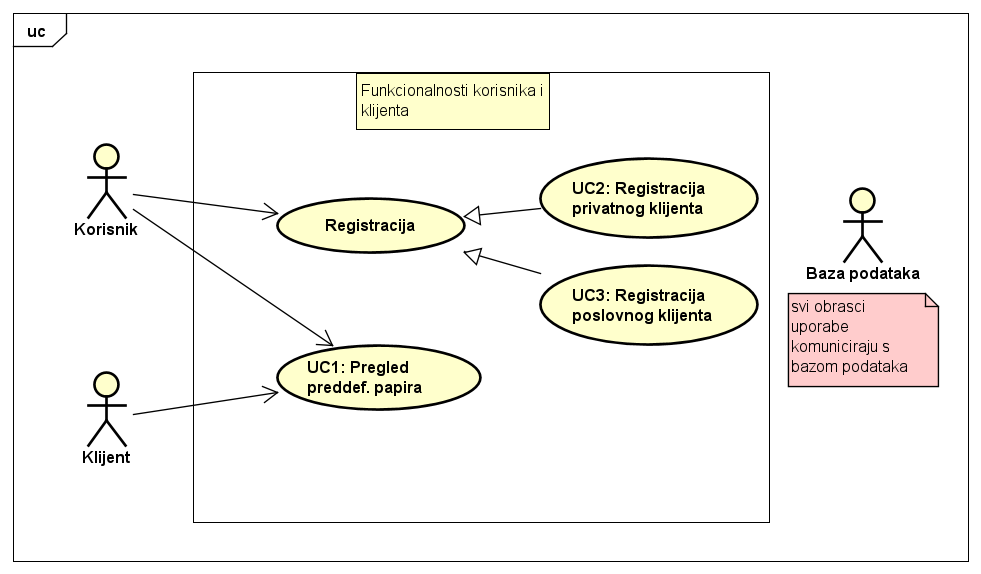
\includegraphics[scale=0.7]{dijagrami/korisnik_klijent.PNG} 
							\centering
							\caption{Dijagram obrazaca uporabe za korisnika i klijenta}
							\label{fig:obr_up1}%label mora biti drugaciji za svaku sliku
						\end{figure}
						
						\noindent \normalsize{   } \\
						\begin{figure}[H]
							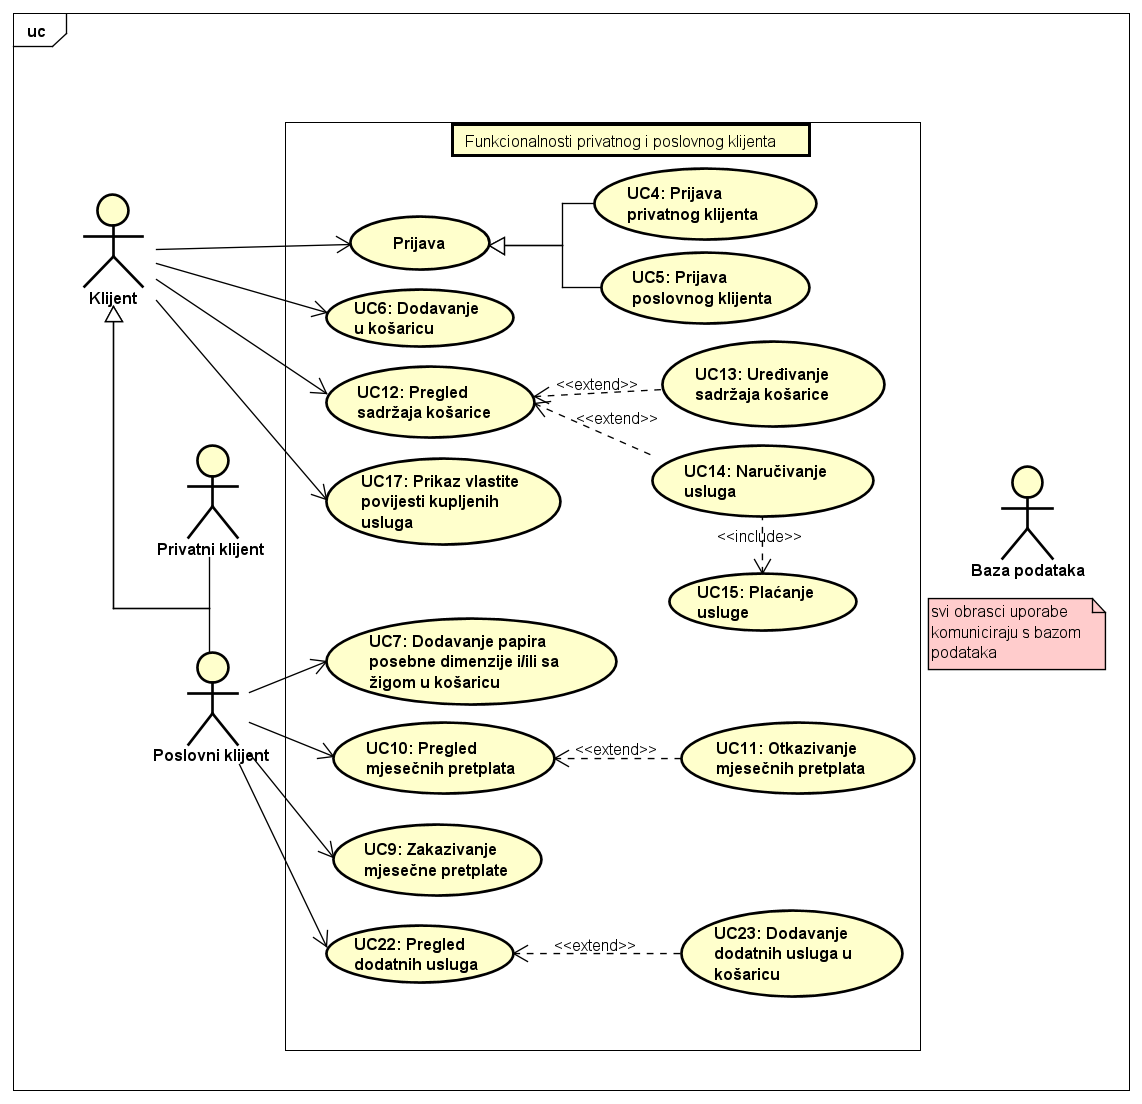
\includegraphics[scale=0.6]{dijagrami/privatni_poslovni.PNG} 
							\centering
							\caption{Dijagram obrazaca uporabe za privatne i poslovne klijente}
							\label{fig:obr_up2}%label mora biti drugaciji za svaku sliku
						\end{figure}
						\noindent \normalsize{   } \\
						\begin{figure}[H]
							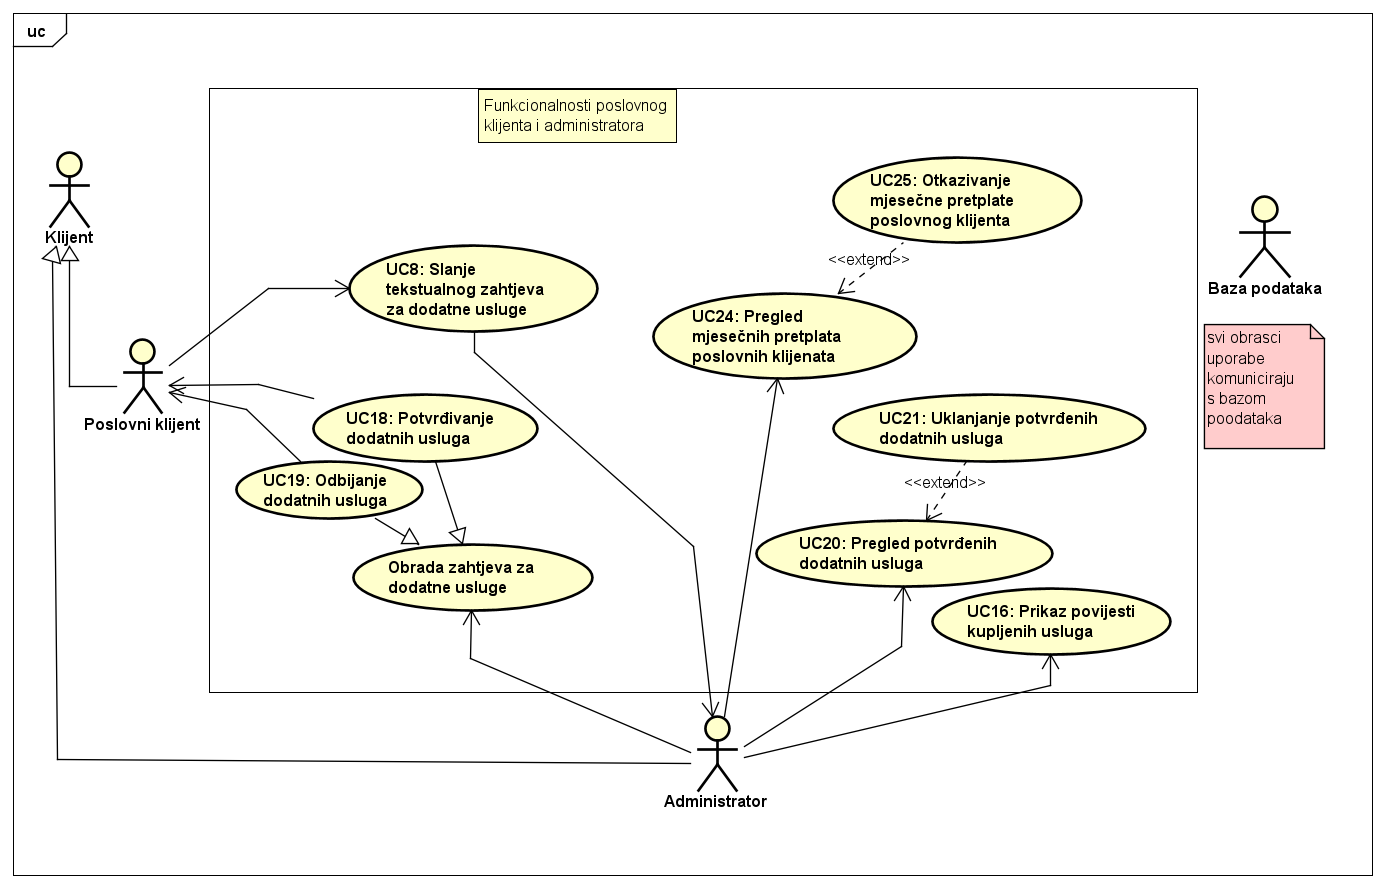
\includegraphics[scale=0.5]{dijagrami/poslovni_admin.PNG} 
							\centering
							\caption{Dijagram obrazaca uporabe za poslovne klijente i administratora}
							\label{fig:obr_up3}%label mora biti drugaciji za svaku sliku
						\end{figure}
						
					\end{center}
					
				\eject		
				
			\subsection{Sekvencijski dijagrami}
				
				\textbf{UC6: Dodavanje u košaricu}\\
				\noindent \normalsize{Klijent odabire parametre za željeni papir i stisne na gumb za dodavanje u košaricu. Ako su uneseni parametri ispravni (uneseni su svi i u pravilnom zapisu), onda se papir dodaje u košaricu. U suprotnom klijentu stiže poruka da nije odabrao sve parametre i košarica se ne mijenja.} \\
				\begin{figure}[H]
					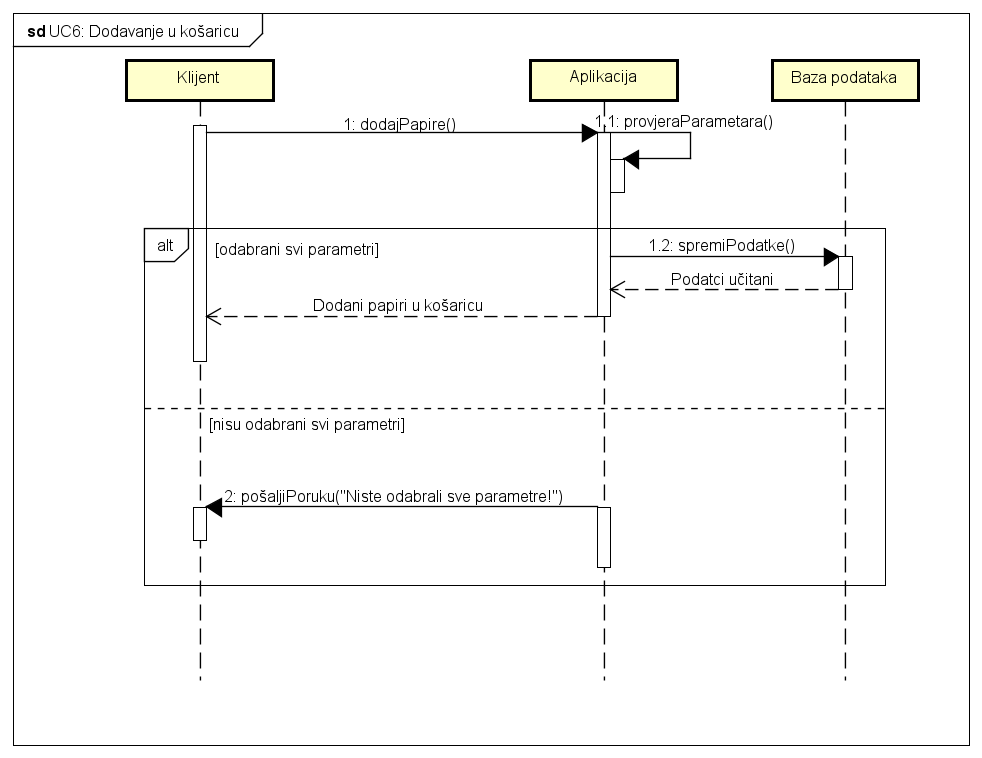
\includegraphics[scale=0.6]{dijagrami/sekv_uc6.PNG} 
					\centering
					\caption{Sekvencijski dijagram za UC6 - Dodavanje u košaricu}
					\label{fig:sekv_uc6}%label mora biti drugaciji za svaku sliku
				\end{figure}
			%	\textit{Nacrtati sekvencijske dijagrame koji modeliraju najvažnije dijelove sustava (max. 4 dijagrama). Ukoliko postoji nedoumica oko odabira, razjasniti s asistentom. Uz svaki dijagram napisati detaljni opis dijagrama.}
			\textbf{UC11: Otkazivanje mjesečnih pretplata}\\
			\noindent \normalsize{Poslovni klijent odabire pregled svojih pretplata. Ako pretplate postoje, one se prikazuju i klijent tada može otkazati bilo koju od njih. Kada se pretplata uspješno otkaže, klijentu dolazi poruka da je pretplata otkazana. U slučaju da klijent nema niti jednu pretplatu, dolazi mu poruka da nema pretplata i stoga ne može ništa otkazati.} \\
			\begin{figure}[H]
				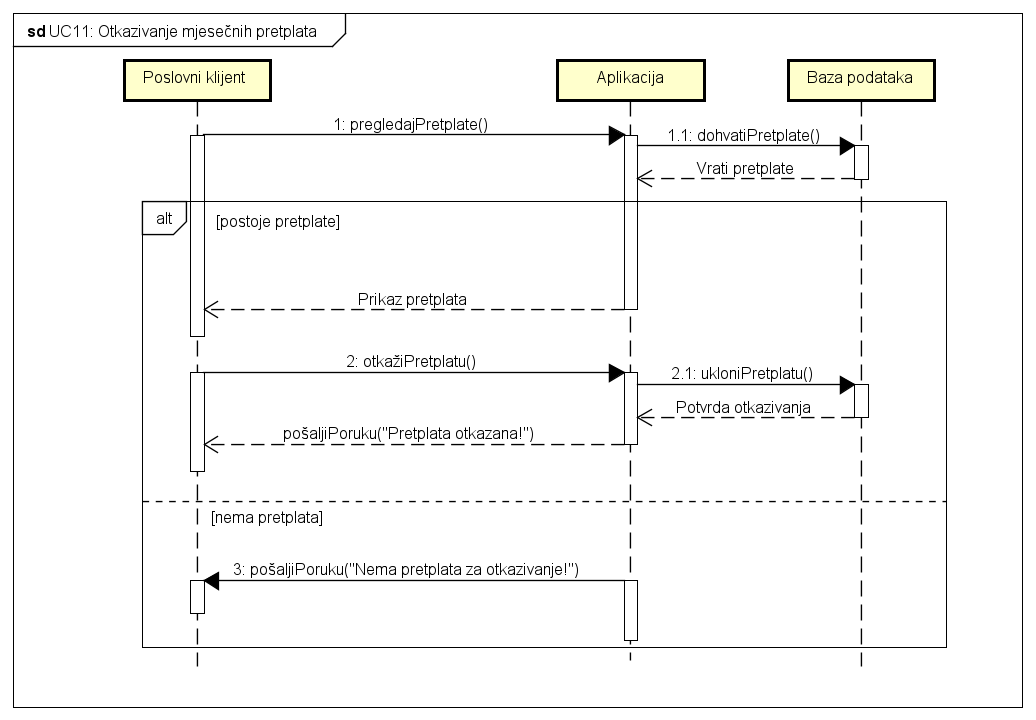
\includegraphics[scale=0.6]{dijagrami/sekv_uc11.PNG} 
				\centering
				\caption{Sekvencijski dijagram za UC11 - Otkazivanje mjesečnih pretplata}
				\label{fig:sekv_uc11}%label mora biti drugaciji za svaku sliku
			\end{figure}
		
			\textbf{UC14: Naručivanje usluga}\\
			\noindent \normalsize{Klijent odabire pregled košarice. Ako košarica nije prazna, prikazuje se njezin sadržaj i tada klijent može potvrditi narudžbu. U suprotnom, dolazi mu poruka da je košarica prazna (nema opciju  potvrditi narudžbu.)} \\
			\begin{figure}[H]
				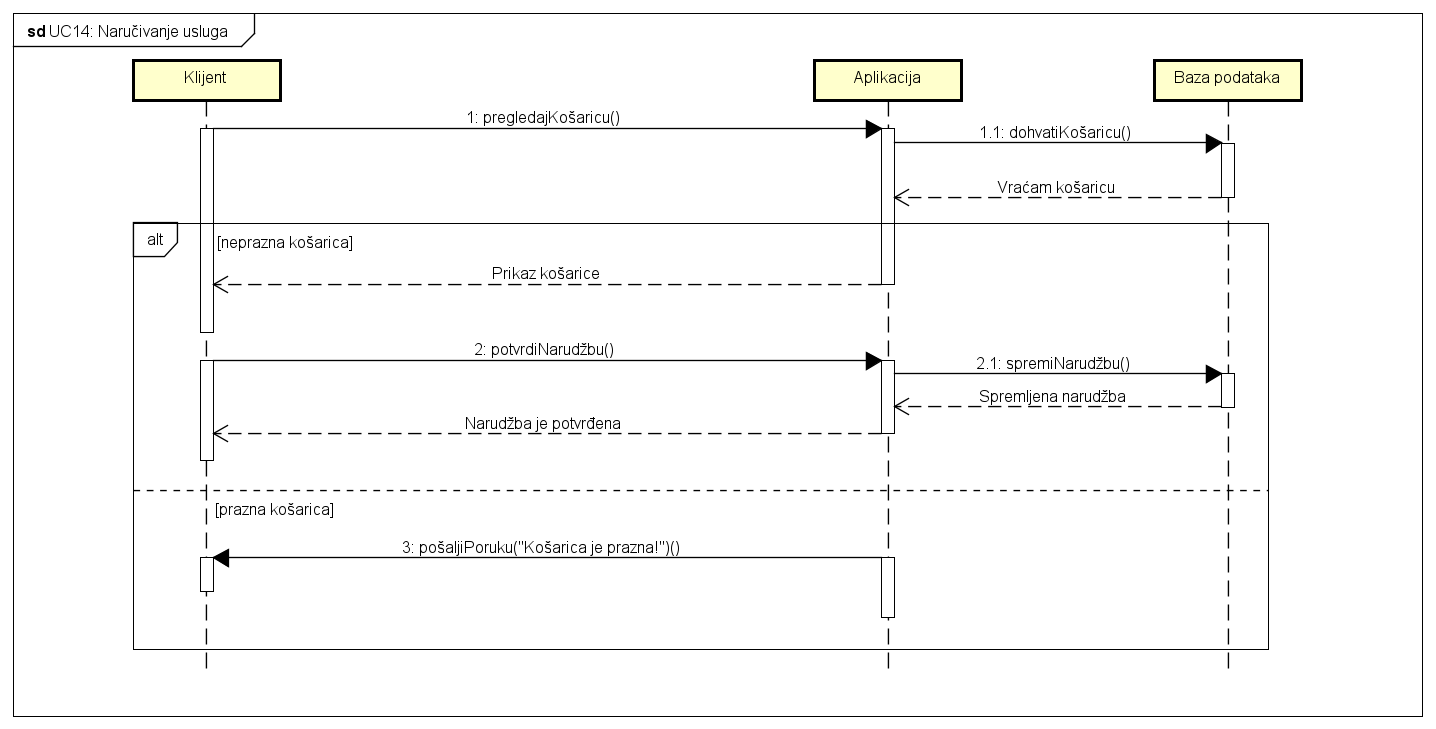
\includegraphics[scale=0.5]{dijagrami/sekv_uc14.PNG} 
				\centering
				\caption{Sekvencijski dijagram za UC14 - Naručivanje usluga}
				\label{fig:sekv_uc14}%label mora biti drugaciji za svaku sliku
			\end{figure}
		
			\textbf{UC25: Otkazivanje mjesečne pretplate poslovnih klijenata}\\
			\noindent \normalsize{Administrator odabire prikaz svih pretplata postojećih poslovnih klijenata. Među njima odabire neku pretplatu nekog od njih i otkazuje ju. Time se ta pretplata za tog klijenta briše.} \\
			\begin{figure}[H]
				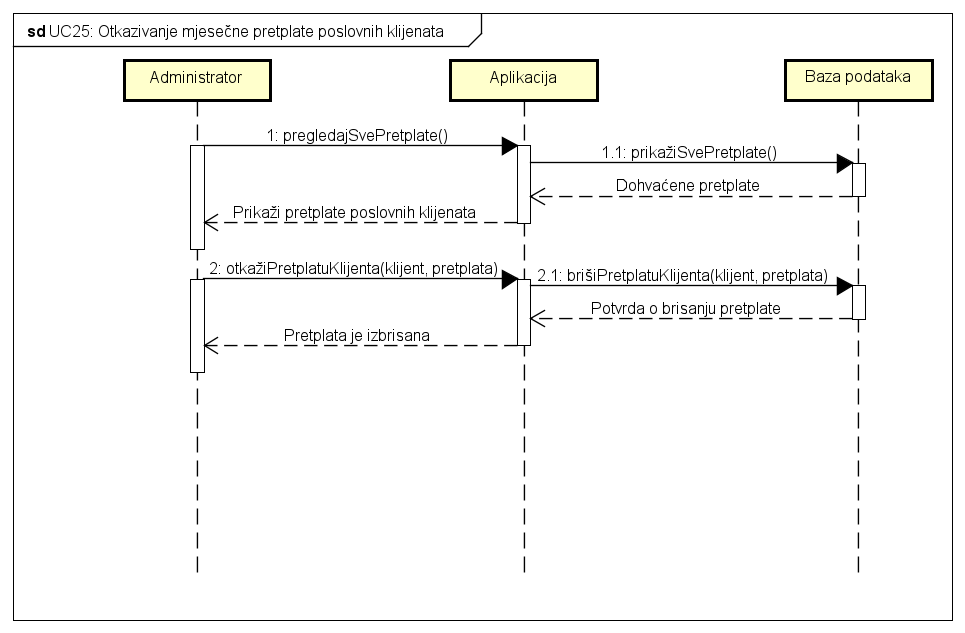
\includegraphics[scale=0.6]{dijagrami/sekv_uc25.PNG} 
				\centering
				\caption{Sekvencijski dijagram za UC25 - Otkazivanje mjesečne pretplate poslovnih klijenata}
				\label{fig:sekv_uc25}%label mora biti drugaciji za svaku sliku
			\end{figure}
				\eject
	
		\section{Ostali zahtjevi}
		
			%\textbf{\textit{dio 1. revizije}}\\
		 
			% \textit{Nefunkcionalni zahtjevi i zahtjevi domene primjene dopunjuju funkcionalne zahtjeve. Oni opisuju \textbf{kako se sustav treba ponašati} i koja \textbf{ograničenja} treba poštivati (performanse, korisničko iskustvo, pouzdanost, standardi kvalitete, sigurnost...). Primjeri takvih zahtjeva u Vašem projektu mogu biti: podržani jezici korisničkog sučelja, vrijeme odziva, najveći mogući podržani broj korisnika, podržane web/mobilne platforme, razina zaštite (protokoli komunikacije, kriptiranje...)... Svaki takav zahtjev potrebno je navesti u jednoj ili dvije rečenice.}
			
			\begin{packed_enum}
				
			
				\item Pristupanje bazi podataka ne smije trajati predugo (više od nekoliko sekundi)
				\item Sustav treba omogućiti rad više korisnika u stvarnom vremenu
				\item Nadogradnje sustava ne smiju narušavati funkcionalnosti sustava koje već postoje
				\item Sustav će biti implementiran u obliku aplikacije koristeći objektno-orijentirane jezike
				\item Aplikacija treba biti jednostavna i intuitivna za korištenje
				\item Kao valutu aplikacija koristi hrvatsku kunu - HRK 
				
				%% sadržaj će biti dodan još i prije 2. rev
				
				
			\end{packed_enum}
			 
			 
			 
	
	\chapter{Arhitektura i dizajn sustava}
		
		%\textbf{\textit{dio 1. revizije}}\\

		%\textit{ Potrebno je opisati stil arhitekture te identificirati: podsustave, preslikavanje na radnu platformu, spremišta podataka, mrežne protokole, globalni upravljački tok i sklopovsko-programske zahtjeve. Po točkama razraditi i popratiti odgovarajućim skicama:}
	%\begin{itemize}
	%	\item 	\textit{izbor arhitekture temeljem principa oblikovanja pokazanih na predavanjima (objasniti zašto ste baš odabrali takvu arhitekturu)}
	%	\item 	\textit{organizaciju sustava s najviše razine apstrakcije (npr. klijent-poslužitelj, baza podataka, datotečni sustav, grafičko sučelje)}
	%	\item 	\textit{organizaciju aplikacije (npr. slojevi frontend i backend, MVC arhitektura) }		
	%\end{itemize}

	Odabrani stil je arhitektura zasnovana na događajima, točnije obrazac MVC (eng. Model-View-Controller) koji je podržan u Spring razvojnom okviru korištenjem anotacija (eng. annotations).
	
	Arhitektura se može podijeliti na tri podsustava:
	\begin{itemize}
		\item Web poslužitelj
		\item Mobilna aplikacija
		\item Baza podataka
	\end{itemize}
	
	\underline{Mobilna aplikacija} je program dizajniran za izvođenje specifičnih funkcija na mobilnom uređaju (npr. pametnom telefonu, tabletu, pametnom satu, itd.). Preko mobilne aplikacije se provodi interakcija sa korisnikom i slanje zatjeva web poslužitelju.

	\underline {Web poslužitelj} je program kojem je zadaća komunikacija sa mobilnom aplikacijom i obrada poslanih zahtjeva. Komunikacija između web poslužitelja i mobilne aplikacije se odvija na World Wide Webu koristeći HTTP (Hypertext Transfer Protocol) protokol za prijenos informacija.
	
	Korišteni programski jezik za izradu poslužiteljske aplikacije je Java sa radnim okvirom (eng. framework) Spring, dok je za izradu mobilne aplikacije korišten Dart.
	
	MVC obrazac je odabran zato što olakšava nazavisan razvoj, ispitivanje i nadogradnju dijelova aplikacije različitih namjena.
	MVC obrazac se sadrži:
	\begin{itemize}
		\item\textbf{Model} - Središnja komponenta sustava. Dinamička struktura podataka aplikacije, neovisna o korisničkom sučelju. Upravlja podacima, logikom i pravilima aplikacije.
		\item\textbf{View (Pogled)} - Bilo kakav prikaz podataka, kao što su graf, dijagram i tablica. Različiti prikazi iste informacije su mogući.
		\item\textbf{Controller (Nadglednik)} - Upravlja i rukuje korisničkom interakcijom sa modelom i pogledom (eng. vIew). Šalje naloge za korištenje podataka modelu, a pogledu šalje naloge za izmjenu prikaza.
	\end{itemize}

				
		\section{Baza podataka}
			
			%\textbf{\textit{dio 1. revizije}}\\
			
		%\textit{Potrebno je opisati koju vrstu i implementaciju baze podataka ste odabrali, glavne komponente od kojih se sastoji i slično.}
		
		Koristit ćemo relacijsku bazu podataka koja svojom strukturom zadovoljava naručiteljeve zahtjeve i olakšava korištenje. Gradivna jedinka baze je relacija, odnosno tablica koja je definirana svojim imenom i skupom atributa. Zadaća baze podataka je brza i jednostavna pohrana, izmjena i dohvat podataka za daljnju obradu. Baza podataka ove aplikacije sastoji se od sljedećih entiteta:
		\begin{itemize}
			\item Korisnik %*možda dodati tablicu klijent koja ima PayPal podatke
			\item Tvrtka
			\item Narudžba
			\item Redovna usluga
			\item Dodatna usluga
			\item Format papira
			\item Vrsta papira
			\item Boja papira
			\item Sadrži dodatnu
			\item Poruka pretplate
			\item Osnovna cijena
		\end{itemize}
			\subsection{Opis tablica}
			%\usepackage{color, colortbl}
		

				%\textit{Svaku tablicu je potrebno opisati po zadanom predlošku. Lijevo se nalazi točno ime varijable u bazi podataka, u sredini se nalazi tip podataka, a desno se nalazi opis varijable. Svjetlozelenom bojom označite primarni ključ. Svjetlo plavom označite strani ključ}
				
			%	\begin{longtabu} to \textwidth {|X[6, l]|X[6, l]|X[20, l]|}
					
				%	\hline \multicolumn{3}{|c|}{\textbf{korisnik - ime tablice}}	 \\[3pt] \hline
				%	\endfirsthead
					
					%\hline \multicolumn{3}{|c|}{\textbf{korisnik - ime tablice}}	 \\[3pt] \hline
				%	\endhead
					
				%	\hline 
				%	\endlastfoot
					
				%	\cellcolor{LightGreen}IDKorisnik & INT	&  	Lorem ipsum dolor sit amet, consectetur adipiscing elit, sed do eiusmod tempor incididunt ut labore et dolore magna aliqua. Ut enim ad minim veniam 	\\ \hline
				%	korisnickoIme	& VARCHAR &   	\\ \hline 
				%	email & VARCHAR &   \\ \hline 
				%	ime & VARCHAR	&  		\\ \hline 
				%	\cellcolor{LightBlue} primjer	& VARCHAR &   	\\ \hline 
					
					
			%	\end{longtabu}
				
				\definecolor{Celadon}{RGB}{0.67, 0.88, 0.69} %lijepa zelena
				\definecolor{grannysmithapple}{RGB}{0.66, 0.89, 0.63}  %lijepa zelena
				\definecolor{babyblueeyes}{RGB}{0.63, 0.79, 0.95}  %lijepa plava
				\definecolor{beaublue}{RGB}{0.74, 0.83, 0.9} %lijepa plava
				\definecolor{blizzardblue}{RGB}{0.67, 0.9, 0.93} %lijepa plava
				\definecolor{columbiablue}{RGB}{0.61, 0.87, 1.0} %lijepa plava
				
				
				\definecolor{Celadonm}{HTML}{ACE1AF} %lijepa zelena
				
				\textit{Podebljani atributi su primarni ključevi, dok su podcrtani vanjski ključevi.}
				\\
				
				
				\textbf{Korisnik}\newline  Ovaj entitet sadržava važne informacije o korisniku aplikacije. Sadrži atribute: korisnik\_id, email, lozinka, ime, prezime, razina\_korisnika i tvrtka\_id. Ovaj entitet je u vezi 1:0..1 s entitetom tvrtka preko atributa tvrtka\_id tvrtke, u vezi One-to-Many s entitetom narudžba preko atributa korisnik\_id korisnika i u vezi One-to-Many s entitetom dodatna\_usluga preko atributa korisnik\_id korisnika.
				\begin{longtabu} to \textwidth {|X[8, l]|X[6, l]|X[20, l]|}
					
					\hline \multicolumn{3}{|c|}{\textbf{korisnik}}	 \\[3pt]
					\hline
					\endfirsthead
					
					\hline \multicolumn{3}{|c|}{\textbf{korisnik}}	 \\[3pt]
					\hline
					\endhead
					
					\hline 
					\endlastfoot
					
					\cellcolor{LightGreen}
					\textbf{korisnik\_id}  & SERIAL  & jedinstveni identifikator korisnika\\ \hline
					email	  	 	  & VARCHAR & email koji se koristi pri prijavi	\\ \hline 
					lozinka		 	  & VARCHAR & lozinka koje se koristi i s kojom se uspoređuje pri prijavi \\ \hline 
					ime			 	  & VARCHAR & ime korisnika 						\\ \hline
					prezime		 	  & VARCHAR & prezime korisnika \\ \hline
					razina\_korisnika & INT		& razina korisnika \\
									  &			& 0 - privatni		\\
									  &			& 1 - poslovni		\\
									  &			& 2 - admin		\\ \hline
					\cellcolor{LightBlue}
					\underline{tvrtka\_id}  & INT 	   & id korisnikove tvrtke ako postoji, NULL inače
					
				\end{longtabu}
				
				\textbf{Tvrtka}\newline Ovaj entitet sadrži informacije o tvrtci za poslovne korisnike. Sadrži atribute: tvrtka\_id, tvrtka\_oib, broj\_telefona i korisnik\_id. Ovaj entitet je u vezi One-to-One sa entitetom korisnik preko korisnik\_id korisnika, te 0..1:1 sa entitetom korisnik preko tvrka\_id tvrtke.
				\begin{longtabu} to \textwidth {|X[6, l]|X[6, l]|X[20, l]|}
					
					\hline \multicolumn{3}{|c|}{\textbf{tvrtka}}	 \\[3pt] \hline
					\endfirsthead
					
					\hline \multicolumn{3}{|c|}{\textbf{tvrtka}}	 \\[3pt] \hline
					\endhead
					
					\hline 
					\endlastfoot
					
					\cellcolor{LightGreen}
					\textbf{tvrtka\_id}	& SERIAL  &		jedinstveni identifikator tvrtke	\\ \hline
					tvrtka\_oib		& VARCHAR &		OIB tvrtke							\\ \hline
					ime\_tvrtke		& VARCHAR &  	ime tvrtke							\\ \hline
					broj\_telefona	& VARCHAR &   	broj telefona kontakt osobe tvrtke	\\ \hline 
					\cellcolor{LightBlue}
					\underline{korisnik\_id} 	& INT	  &  	korisnički id tvrtke			 	\\ \hline
					
				\end{longtabu}
				
				\textbf{Narudžba}\newline  Ovaj entitet opisuje osnovne informacije o narudžbi korisnika. Sadrži atribute: narudzba\_id, korisnik\_id, cijena i datum. Ovaj entitet je u vezi Many-to-One s entitetom korisnik preko atributa korisnik\_id korisnika, u vezi One-to-Many s entitetom sadrziDodatnu preko atributa narudzba\_id i korisnik\_id narudzbe, u vezi One-to-Many s entitetom redovna\_usluga preko atributa narudzba\_id i korisnik\_id narudzbe i u vezi One-to-Many s entitetom porukaPretplate preko atributa narudzba\_id i korisnik\_id narudzbe.
				\begin{longtabu} to \textwidth {|X[8, l]|X[6, l]|X[20, l]|}
					
					\hline \multicolumn{3}{|c|}{\textbf{narudzba}}	 \\[3pt] \hline
					\endfirsthead
					
					\hline \multicolumn{3}{|c|}{\textbf{narudzba}}	 \\[3pt] \hline
					\endhead
					
					\hline 
					\endlastfoot
					
					\cellcolor{LightGreen}
					\textbf{narudzba\_id} & SERIAL	& jedinstveni identifikator narudžbe\\ \hline
					\cellcolor{LightBlue}
					\textbf{\underline{korisnik\_id}}  & INT &  jedinstveni identifikator korisnika naručitelja 	\\ \hline
					cijena 			& NUMERIC & cijena narudžbe					   	\\ \hline  
					datum 			& TIMESTAMP	& datum i vrijeme provedbe narudžbe	\\ \hline 
					
				\end{longtabu}
				
				\textbf{Dodatna usluga}\newline  Ovaj entitet opisuje sve informacije o dodatnoj usluzi za pojedinog korisnika. Sadrži atribute: dodatna\_usluga\_id, korisnik\_id, dodatna\_naziv, dodatna\_opis, cijena, kontakt\_ime, kontakt\_broj, kontakt\_email, potvrdena i pretplata. Entitet je u vezi Many-to-One s entitetom korisnik preko atributa korisnik\_id korisnika i u vezi One-to-Many s entitetom sadrziDodatnu preko atributa dodatna\_usluga\_id i korisnik\_id dodatne usluge.
				\begin{longtabu} to \textwidth {|X[10, l]|X[6, l]|X[20, l]|}
					
					\hline \multicolumn{3}{|c|}{\textbf{dodatna\_usluga}}	 \\[3pt] \hline
					\endfirsthead
					
					\hline \multicolumn{3}{|c|}{\textbf{dodatna\_usluga}}	 \\[3pt] \hline
					\endhead
					
					\hline 
					\endlastfoot
					
					\cellcolor{LightGreen}
					\textbf{dodatna\_usluga\_id} & SERIAL & jedinstveni identifikator dodatne usluge\\ \hline
					\cellcolor{LightBlue}
					\textbf{\underline{korisnik\_id}}	& INT & jedinstveni identifikator poslovnog korisnika kojem 											je usluga dodijeljena				\\ \hline 
					dodatna\_naziv	& VARCHAR & kratki naziv dodatne usluge		  						\\ \hline 
					dodatna\_opis	& VARCHAR & opis dodatne usluge										\\ \hline 
					cijena 			& NUMERIC & cijena dodatne usluge			   						\\ \hline
					kontakt\_ime 	& VARCHAR & ime kontakt osobe kompanije 							\\ \hline 
					kontakt\_broj 	& VARCHAR & broj kontakt osobe kompanije							\\ \hline 
					kontakt\_email	& VARCHAR & email kontakt osobe kompanije							\\ \hline
					potvrdena		& BOOLEAN & označava je li zahtjev potvrđen ili nije,				\\
					&		  &	ako je true onda je prihvaćen,							\\
					&		  &	ako je false onda administrator još nije donio odluku.	\\
					&		  & U slučaju da je odbijen onda entitet uklanja iz tablice 	\\ \hline
					pretplata		& BOOLEAN & označava je li narudžba mjesečna pretplata				\\ \hline
					
				\end{longtabu}
				
				\textbf{Sadrži dodatnu}\newline Entitet sadrziDodatnu sadrži informaciju koju/koje dodatne usluge sadrži narudžba. Sadrži atribute: narudzba\_id, korisnik\_id, dodatna\_usluga\_id i pretplata. Entitet sadrži vezu Many-to-One s entitetom narudzba preko atributa narudzba\_id i korisnik\_id narudžbe i vezu Many-to-One s entitetom dodatna\_usluga preko atributa dodatna\_usluga\_id i korisnik\_id dodatne usluge.
				\begin{longtabu} to \textwidth {|X[11, l]|X[6, l]|X[20, l]|}
					
					\hline \multicolumn{3}{|c|}{\textbf{sadrziDodatnu}}	 \\[3pt] \hline
					\endfirsthead
					
					\hline \multicolumn{3}{|c|}{\textbf{sadrziDodatnu}}	 \\[3pt] \hline
					\endhead
					
					\hline 
					\endlastfoot
					
					\cellcolor{LightBlue}
					\textbf{\underline{narudzba\_id}} & INT & jedinstveni identifikator narudžbe					\\ \hline
					\cellcolor{LightBlue}
					\textbf{\underline{korisnik\_id}}  & INT &  jedinstveni identifikator korisnika naručitelja 	\\ \hline
					\cellcolor{LightBlue}
					\textbf{\underline{dodatna\_usluga\_id}}		& INT & jedinstveni identifikator dodatne usluge			\\ \hline
					\cellcolor{LightBlue}
					pretplata	& BOOLEAN & označava je li narudžba mjesečna pretplata \\ \hline
				\end{longtabu}
				
				\textbf{Redovna usluga}\newline  Ovaj entitet opisuje redovnu uslugu korisnika. Sadrži entitete: narudzba\_id, korisnik\_id, visina, sirina, boja, tezina, vodeni\_zig, pretplata, format\_id, vrsta\_id i boja\_id. Entitet je u vezi Many-to-One s entitetom narudza preko atributa narudzba\_id i korisnik\_id narudžbe, u vezi Many-to-One sa format\_papira preko atributa format\_id formata papira, u vezi Many-to-One sa vrsta\_papira preko atributa vrsta\_id vrste papira, u vezi Many-to-One sa boja\_papira preko atributa boja\_id boje papira,
				\begin{longtabu} to \textwidth {|X[8, l]|X[6, l]|X[20, l]|}
					
					\hline \multicolumn{3}{|c|}{\textbf{redovna\_usluga}}	 \\[3pt] \hline
					\endfirsthead
					
					\hline \multicolumn{3}{|c|}{\textbf{redovna\_usluga}}	 \\[3pt] \hline
					\endhead
					
					\hline 
					\endlastfoot
					
					\cellcolor{LightBlue}
					\underline{narudzba\_id} 	& SERIAL  & jedinstveni identifikator narudzbe						\\ \hline
					\cellcolor{LightBlue}
					\underline{korisnik\_id}	& INT 	  & jedinstveni identifikator korisnika naručitelja			\\ \hline 
					visina			& INT	  & visina papira u mm		  								\\ \hline 
					sirina			& INT	  & širina papira u mm										\\ \hline 
					boja 			& VARCHAR & heksadecimalni zapis boje papira   						\\ \hline
					tezina		 	& VARCHAR & težina papira u gsm			 							\\ \hline
					vodeni\_zig		& BLOB	  & slika vodenog žiga										\\ \hline
					pretplata		& BOOLEAN & označava je li narudžba mjesečna pretplata				\\ \hline
					\cellcolor{LightBlue}
					\underline{format\_id} 		& INT 	  & jedinstveni identifikator formata papira,				\\
					&		  &	0 je rezerviran za nekonvencionalne formate 			\\ \hline
					\cellcolor{LightBlue}
					\underline{vrsta\_id} 		& INT	  & jedinstveni identifikator vrste papira					\\ \hline
					\cellcolor{LightBlue}
					\underline{boja\_id} 		& INT	  & jedinstveni identifikator boje papira					\\
					&		  &	0 je rezerviran za proizvoljne boje						\\ \hline  
					
					
					
				\end{longtabu}
				
				\textbf{Format papira}\newline	Ovaj entitet sadrži sve informacije o formatu papira. Sadrži atribute format\_id, format\_ime, visina, sirina i koeficijent\_cijena. Entitet je u vezi One-to-Many s entitetom redovna\_usluga preko atributa format\_id formata papira.
				\begin{longtabu} to \textwidth {|X[8, l]|X[6, l]|X[20, l]|}
					
					\hline \multicolumn{3}{|c|}{\textbf{format\_papira}}	 \\[3pt] \hline
					\endfirsthead
					
					\hline \multicolumn{3}{|c|}{\textbf{format\_papira}}	 \\[3pt] \hline
					\endhead
					
					\hline 
					\endlastfoot
					
					\cellcolor{LightGreen}
					\textbf{format\_id} 			& SERIAL  & jedinstveni identifikator formata papira,			\\
					&		  &	0 je rezerviran za nekonvencionalne formate 		\\ \hline
					format\_ime			& VARCHAR & ime formata papira									\\ \hline 
					visina 				& INT	  & visina formata papira u mm							\\ \hline 
					širina 				& INT	  & širina formata papira u mm							\\ \hline 
					koeficijent\_cijena	& NUMERIC & cijena narudžbe				   						\\ \hline 
					
				\end{longtabu}
				
				\textbf{Vrste papira}\newline	Ovaj entitet sadrži sve informacije o vrsti papira. Sadrži atribute vrsta\_id, vrsta\_ime i koeficijent\_cijena. Entitet je u vezi One-to-Many s entitetom redovna\_usluga preko atributa vrsta\_id vrste papira.
				\begin{longtabu} to \textwidth {|X[8, l]|X[6, l]|X[20, l]|}
					
					\hline \multicolumn{3}{|c|}{\textbf{vrste\_papira}}	 \\[3pt] \hline
					\endfirsthead
					
					\hline \multicolumn{3}{|c|}{\textbf{vrste\_papira}}	 \\[3pt] \hline
					\endhead
					
					\hline 
					\endlastfoot
					
					\cellcolor{LightGreen}
					\textbf{vrsta\_id} 			& SERIAL  & jedinstveni identifikator vrste papira				\\ \hline 
					vrsta\_ime 			& VARCHAR & ime vrste papira									\\ \hline 
					koeficijent\_cijena	& NUMERIC & cijena narudžbe				   						\\ \hline  
					
				\end{longtabu}
				
				\textbf{Boja papira}\newline	Ovaj entitet sadrži sve informacije o boji papira. Sadrži atribute boja\_id, boja\_ime, hexcode i koeficijent\_cijena. Entitet je u vezi One-to-Many s entitetom redovna\_usluga preko atributa boja\_id boje papira.
				\begin{longtabu} to \textwidth {|X[8, l]|X[6, l]|X[20, l]|}
					
					\hline \multicolumn{3}{|c|}{\textbf{boja\_papira}}	 \\[3pt] \hline
					\endfirsthead
					
					\hline \multicolumn{3}{|c|}{\textbf{boja\_papira}}	 \\[3pt] \hline
					\endhead
					
					\hline 
					\endlastfoot
					
					\cellcolor{LightGreen}
					\textbf{boja\_id} 			& SERIAL  & jedinstveni identifikator boje papira				\\
					&		  &	0 je rezerviran za proizvoljne boje					\\ \hline  
					ime\_boja 			& VARCHAR & ime boje papira										\\ \hline 
					koeficijent\_cijena	& NUMERIC & cijena narudžbe				   						\\ \hline
					hexcode				& VARCHAR & heksadecimalni zapis boje papira					\\ 
					
				\end{longtabu}
			
				\textbf{Poruka pretplate}\newline	Ovaj entitet sadrži osnovne informacije o porukama pretplate. Entitet se svakih 24h treba ažurirati i dodati unos za korisnika i narudžbu sa pretplatom koja je naručena na ovaj dan u mjesecu. Nakon što je korisnik primio redak on se treba obrisati, te nepojavljivati nadalje. Narudžba\_id je vanjski ključ na narudžba\_id narudžbe, kako bi znali da se pretplate, redovne\_usluge ili dodatne\_usluge\, nalaze u nekoj narudžbi. Korisnik\_id je vanjski ključ za korisnik\_id korisnika i preko njega jednostavno znamo kojemu korisniku treba biti prikazana poruka.
				Sadrži atribute: id, narudžba\_id i korisnik\_id.
				Entitet je u vezi Many-to-One s entitetom narudzba preko atributa narudzba\_id i korisnik\_id narudžbe.
				\begin{longtabu} to \textwidth {|X[8, l]|X[6, l]|X[20, l]|}
					
					\hline \multicolumn{3}{|c|}{\textbf{porukaPretplate}}	 \\[3pt] \hline
					\endfirsthead
					
					\hline \multicolumn{3}{|c|}{\textbf{porukaPretplate}}	 \\[3pt] \hline
					\endhead
					
					\hline 
					\endlastfoot
					
					\cellcolor{LightGreen}
					\textbf{id} 			& SERIAL  & jedinstveni identifikator mjesečne poruke o provedbi pretplate	\\ \hline  
					\underline{narudzba\_id} 	& INT & jedinstveni identifikator narudžbe\\ \hline 
					\underline{korisnik\_id} 	& INT & jedinstveni identifikator korisnika\\
					
				\end{longtabu}
			
				\textbf{Osnovna cijena}\newline	Ovaj entitet sadrži informaciju o osnovnoj cijeni proizvoda. Sadrži atribut: cijena. Tablica ima samo jedan unos.
				\begin{longtabu} to \textwidth {|X[8, l]|X[6, l]|X[20, l]|}
					
					\hline \multicolumn{3}{|c|}{\textbf{osnovna\_cijena}}	 \\[3pt] \hline
					\endfirsthead
					
					\hline \multicolumn{3}{|c|}{\textbf{osnovna\_cijena}}	 \\[3pt] \hline
					\endhead
					
					\hline 
					\endlastfoot
					
					\cellcolor{LightGreen}
					cijena 	& NUMERIC & osnovna cijena proizvoda koja se množi sa koeficijentima cijena kako bi se dobila cijena neke redovne usluge\\
					
				\end{longtabu}
			\newpage
			
			\subsection{Dijagram baze podataka}
			%	\textit{ U ovom potpoglavlju potrebno je umetnuti dijagram baze podataka. Primarni i strani ključevi moraju biti označeni, a tablice povezane. Bazu podataka je potrebno normalizirati. Podsjetite se kolegija "Baze podataka".}
			
			\begin{figure}[H]
				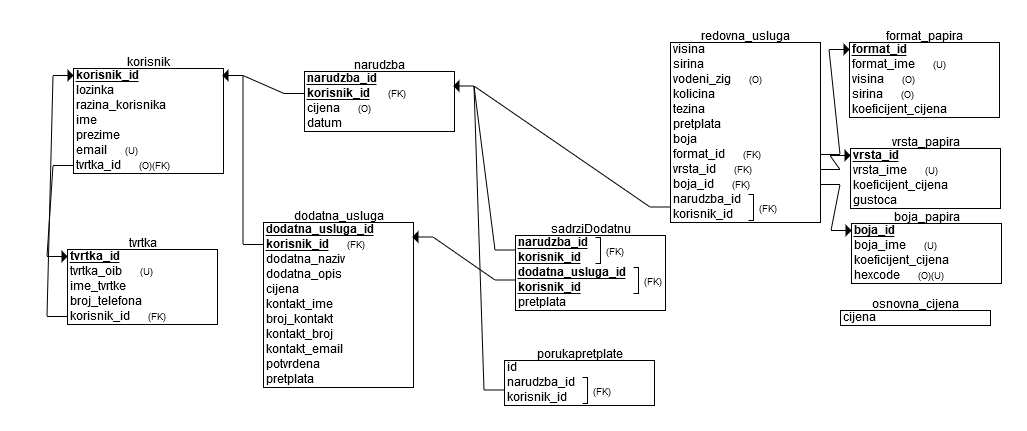
\includegraphics[scale=0.5]{dijagrami/dijagram_baze_podataka.PNG} 
				\centering
				\caption{ER dijagram baze podataka}
				\label{fig:dij_bp1}%label mora biti drugaciji za svaku sliku
			\end{figure}
			
		
		\newpage	
		\section{Dijagram razreda}
		
		%	\textit{Potrebno je priložiti dijagram razreda s pripadajućim opisom. Zbog preglednosti je moguće dijagram razlomiti na više njih, ali moraju biti grupirani prema sličnim razinama apstrakcije i srodnim funkcionalnostima.}\\
			
			%\textbf{\textit{dio 1. revizije}}\\
			
			%\textit{Prilikom prve predaje projekta, potrebno je priložiti potpuno razrađen dijagram razreda vezan uz \textbf{generičku funkcionalnost} sustava. Ostale funkcionalnosti trebaju biti idejno razrađene u dijagramu sa sljedećim komponentama: nazivi razreda, nazivi metoda i vrste pristupa metodama (npr. javni, zaštićeni), nazivi atributa razreda, veze i odnosi između razreda.}\\
			
			%\textbf{\textit{dio 2. revizije}}\\			
			
		%	\textit{Prilikom druge predaje projekta dijagram razreda i opisi moraju odgovarati stvarnom stanju implementacije}
			
			Prikazani razredi se odnose na backend MVC arhitekturu. Dijagram razreda je podijeljen po ulogama na 3 podskupine, controlleri, servici i modeli. Controlleri primaju određene HTTP zahtjeve te pozivaju potrebne servicee koji te zahtjeve dalje obrađuju koristeći potrebne DAO-e (eng. Data Access Object) za komunikaciju sa bazom podataka. Razredi koji se manipuliraju u programu se nalaze u modelu.
			
			\begin{figure}[H]
				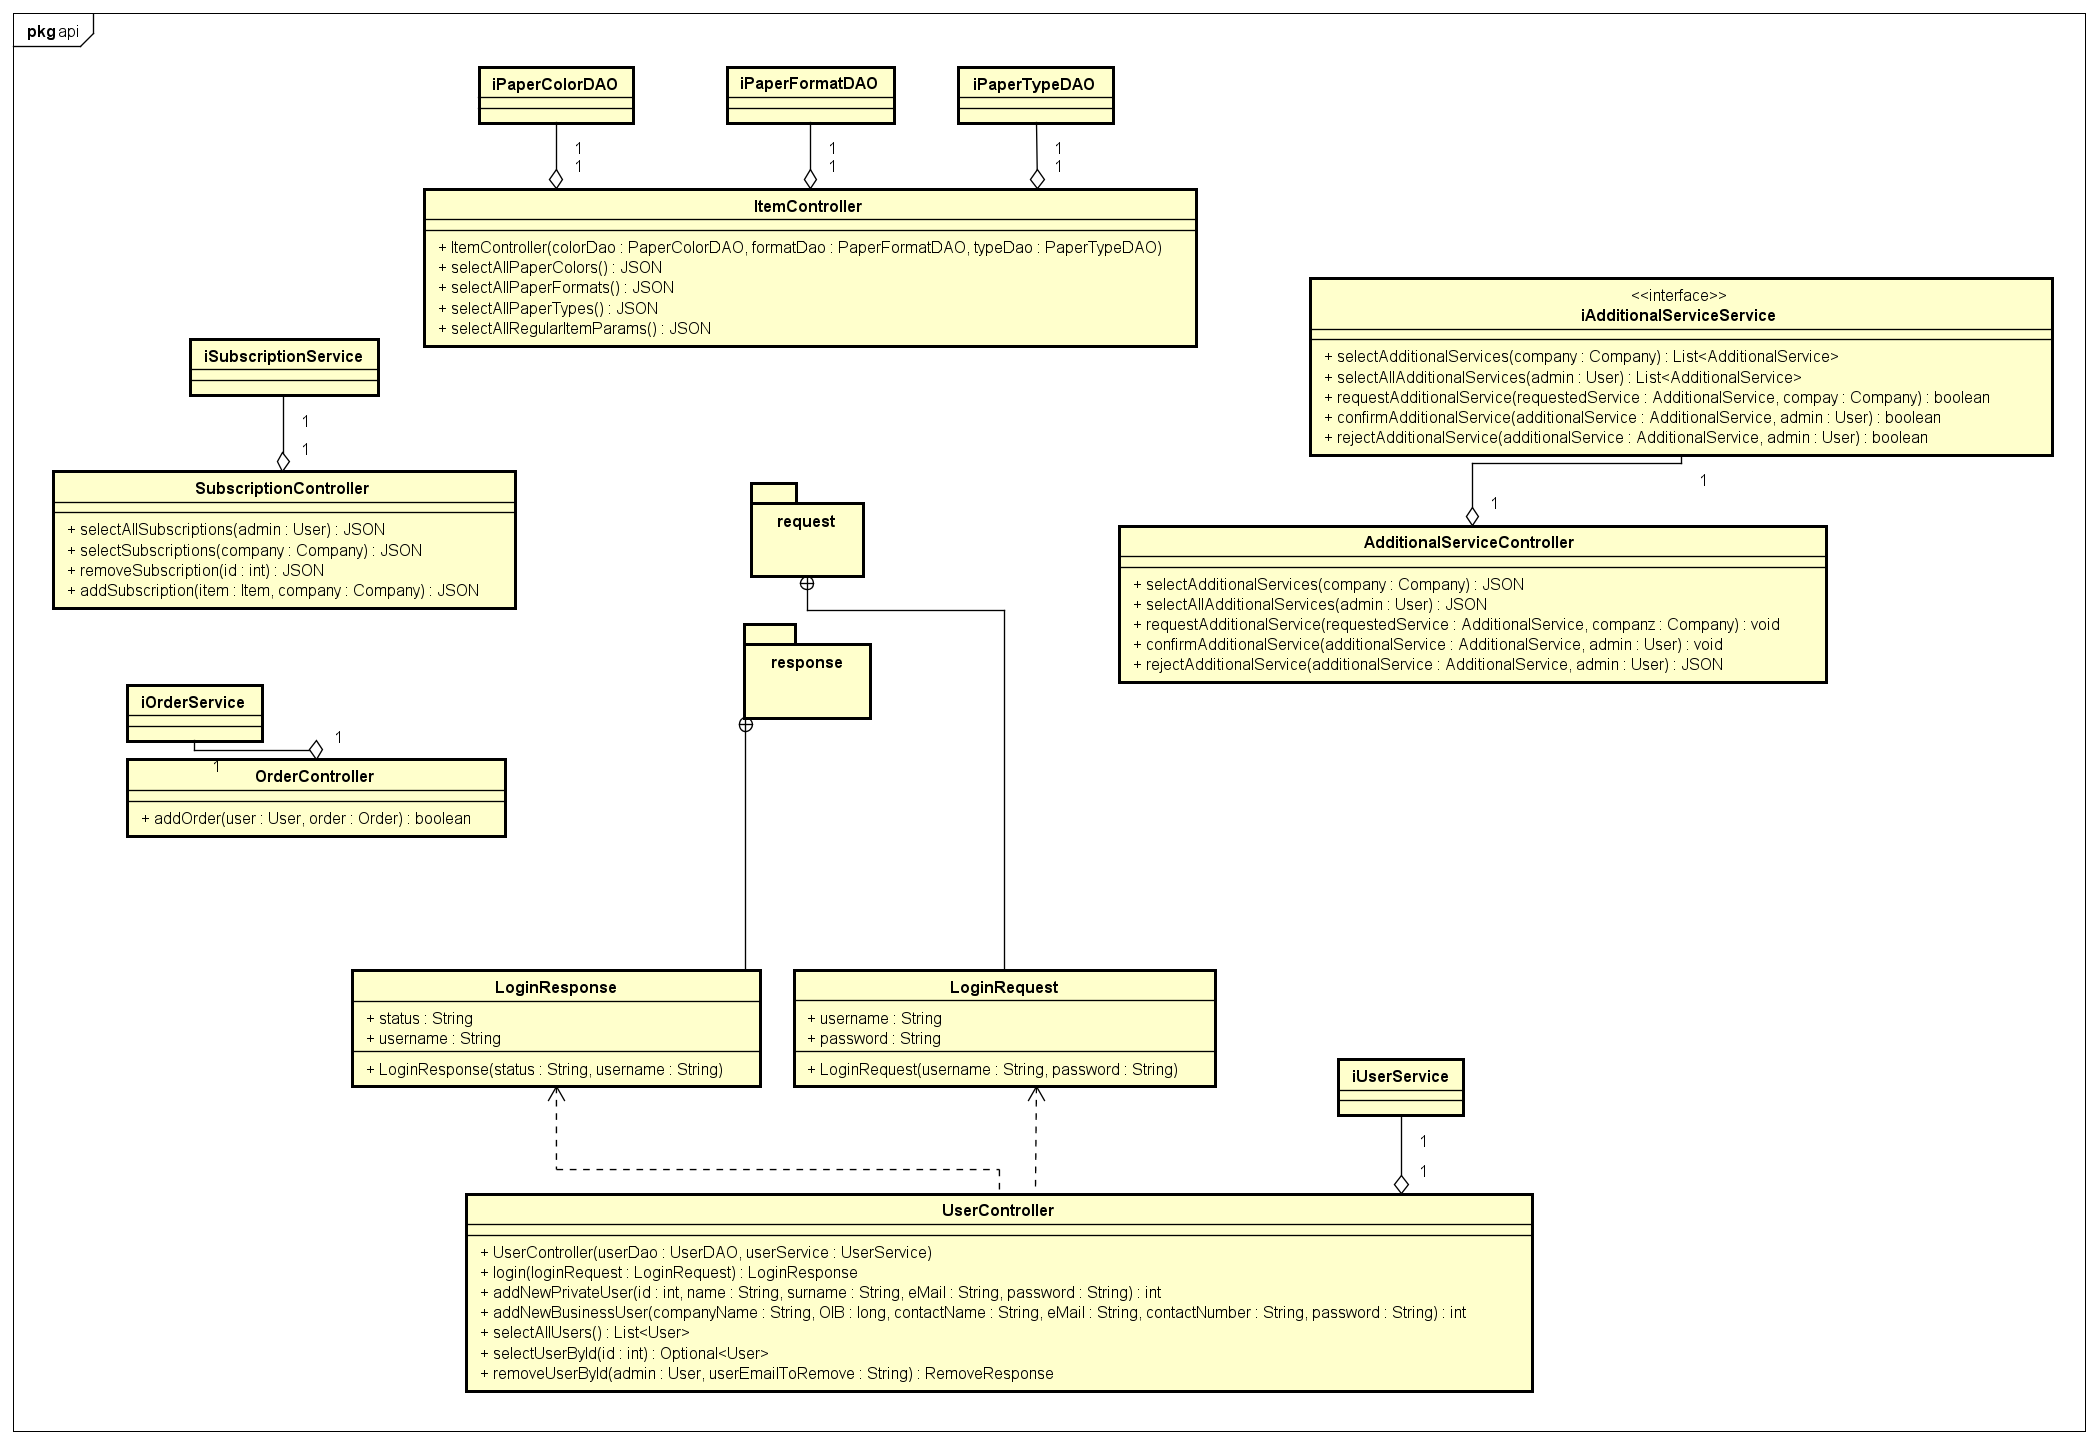
\includegraphics[scale=0.33]{dijagrami/dij_raz_cont.PNG} 
				\centering
				\caption{Dijagram razreda - controlleri}
				\label{fig:dij_raz1}%label mora biti drugaciji za svaku sliku
			\end{figure}
			
			\begin{figure}[H]
				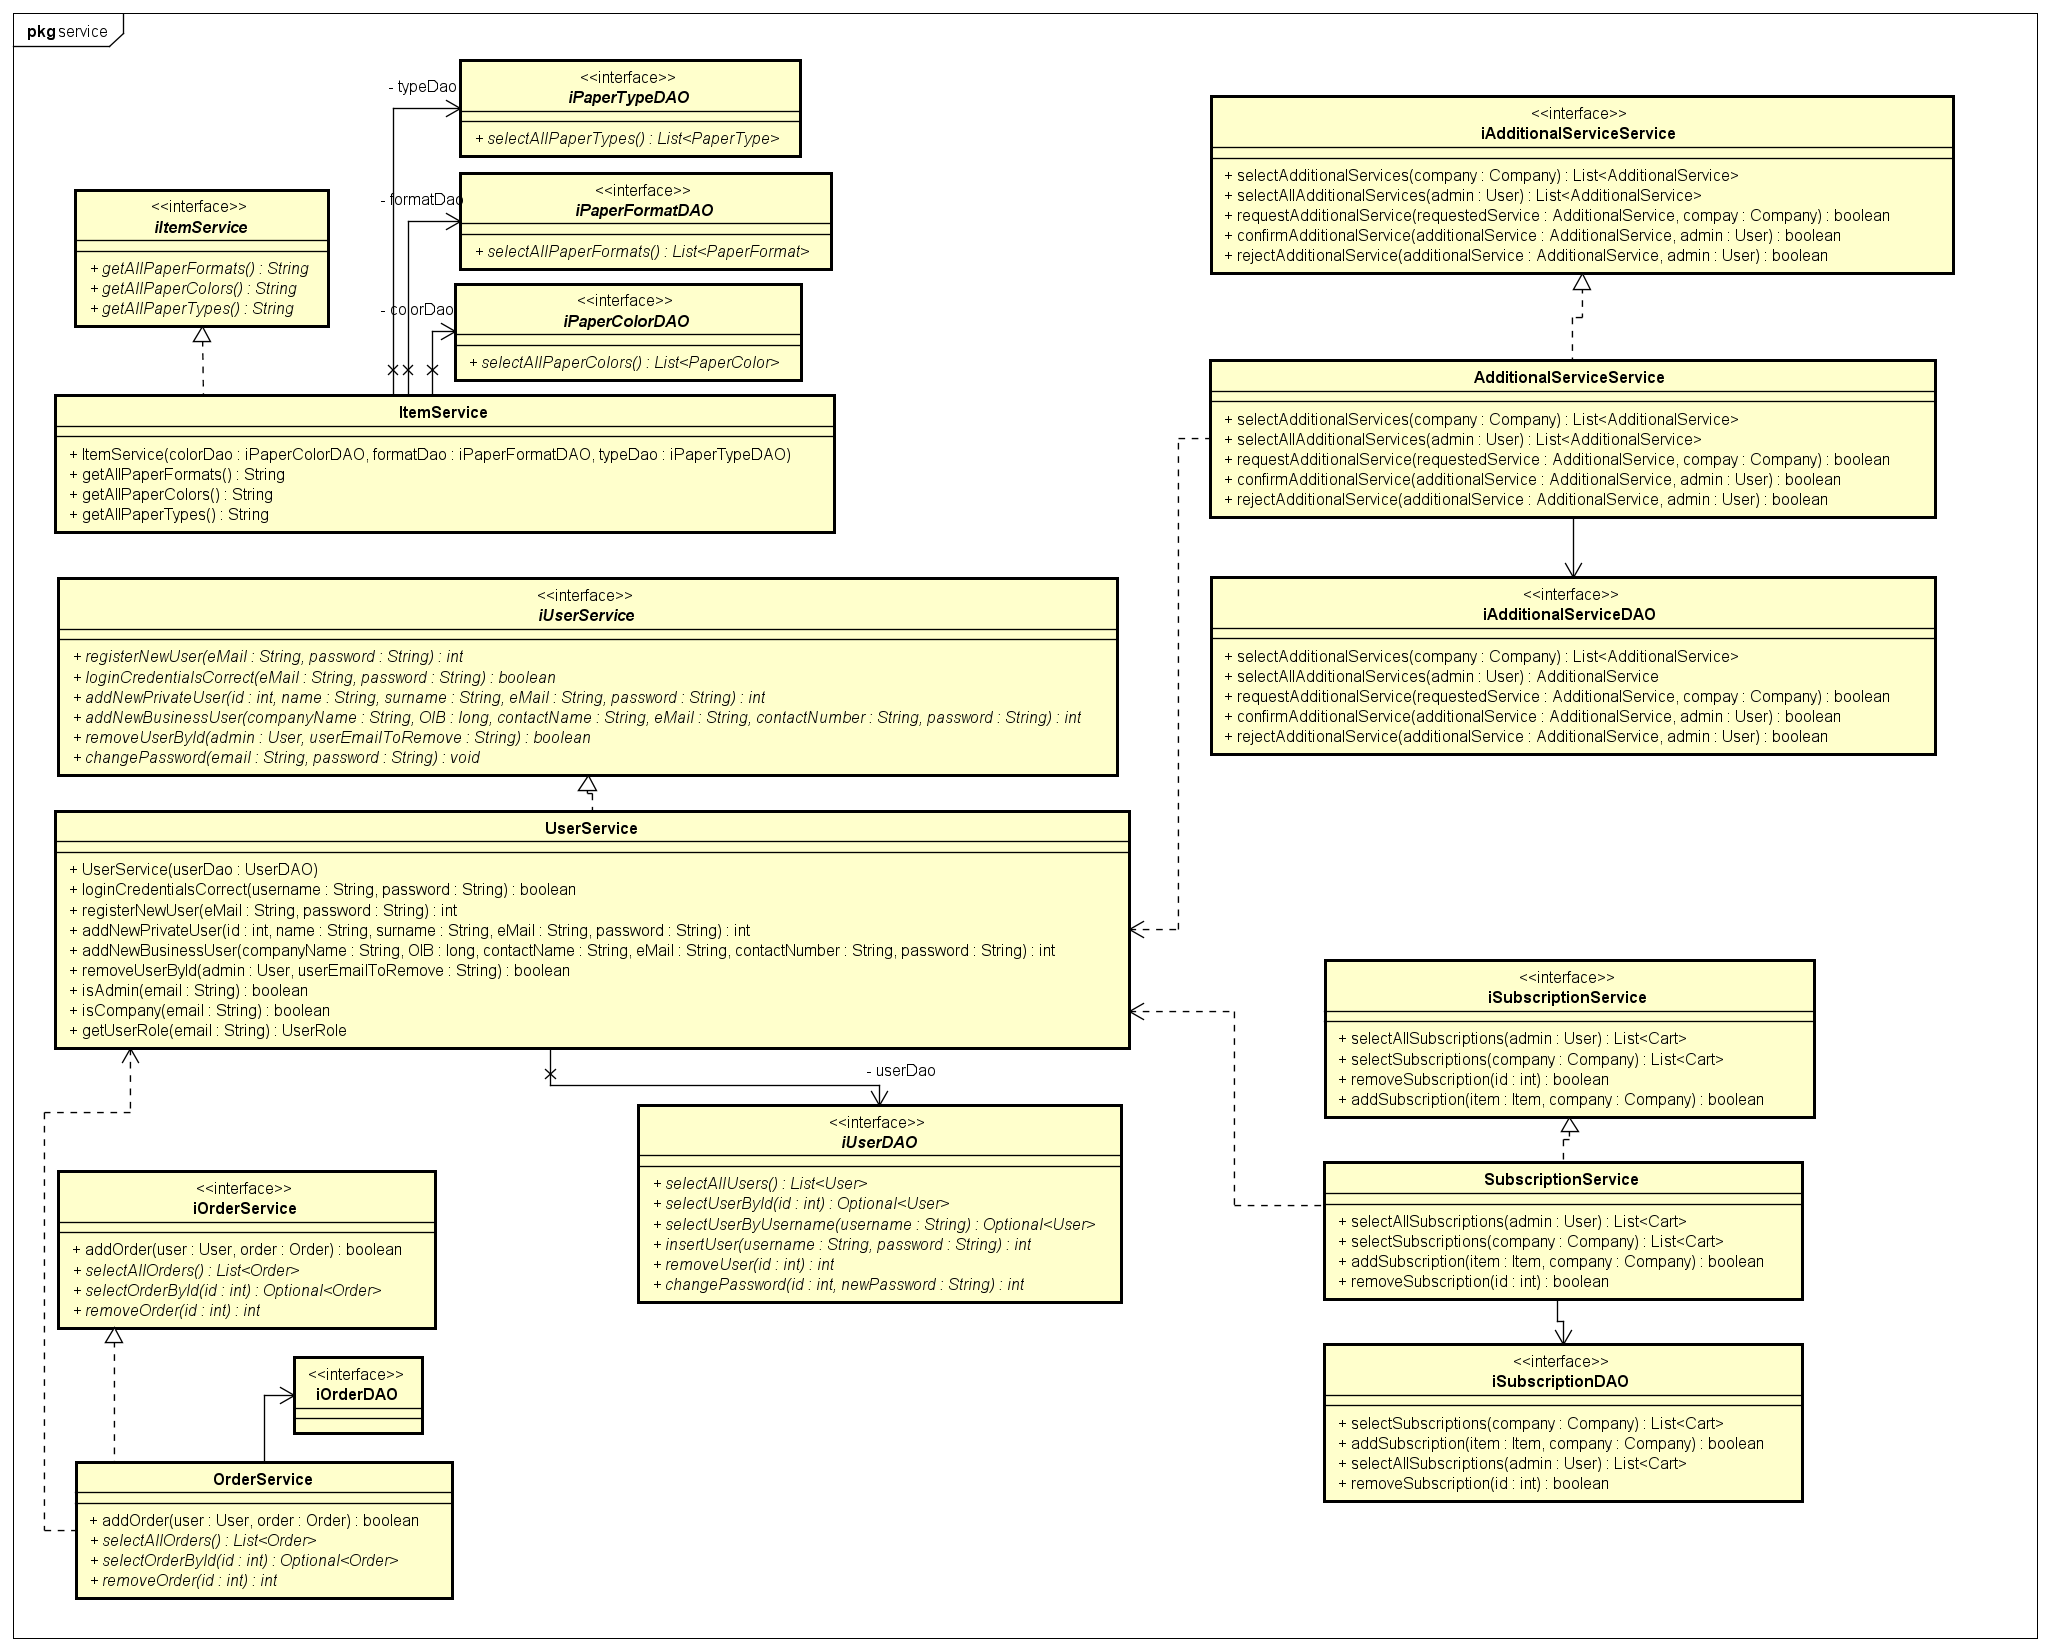
\includegraphics[scale=0.34]{dijagrami/dij_raz_serv.PNG} 
				\centering
				\caption{Dijagram razreda - servici}
				\label{fig:dij_raz2}%label mora biti drugaciji za svaku sliku
			\end{figure}
			
			\begin{figure}[H]
				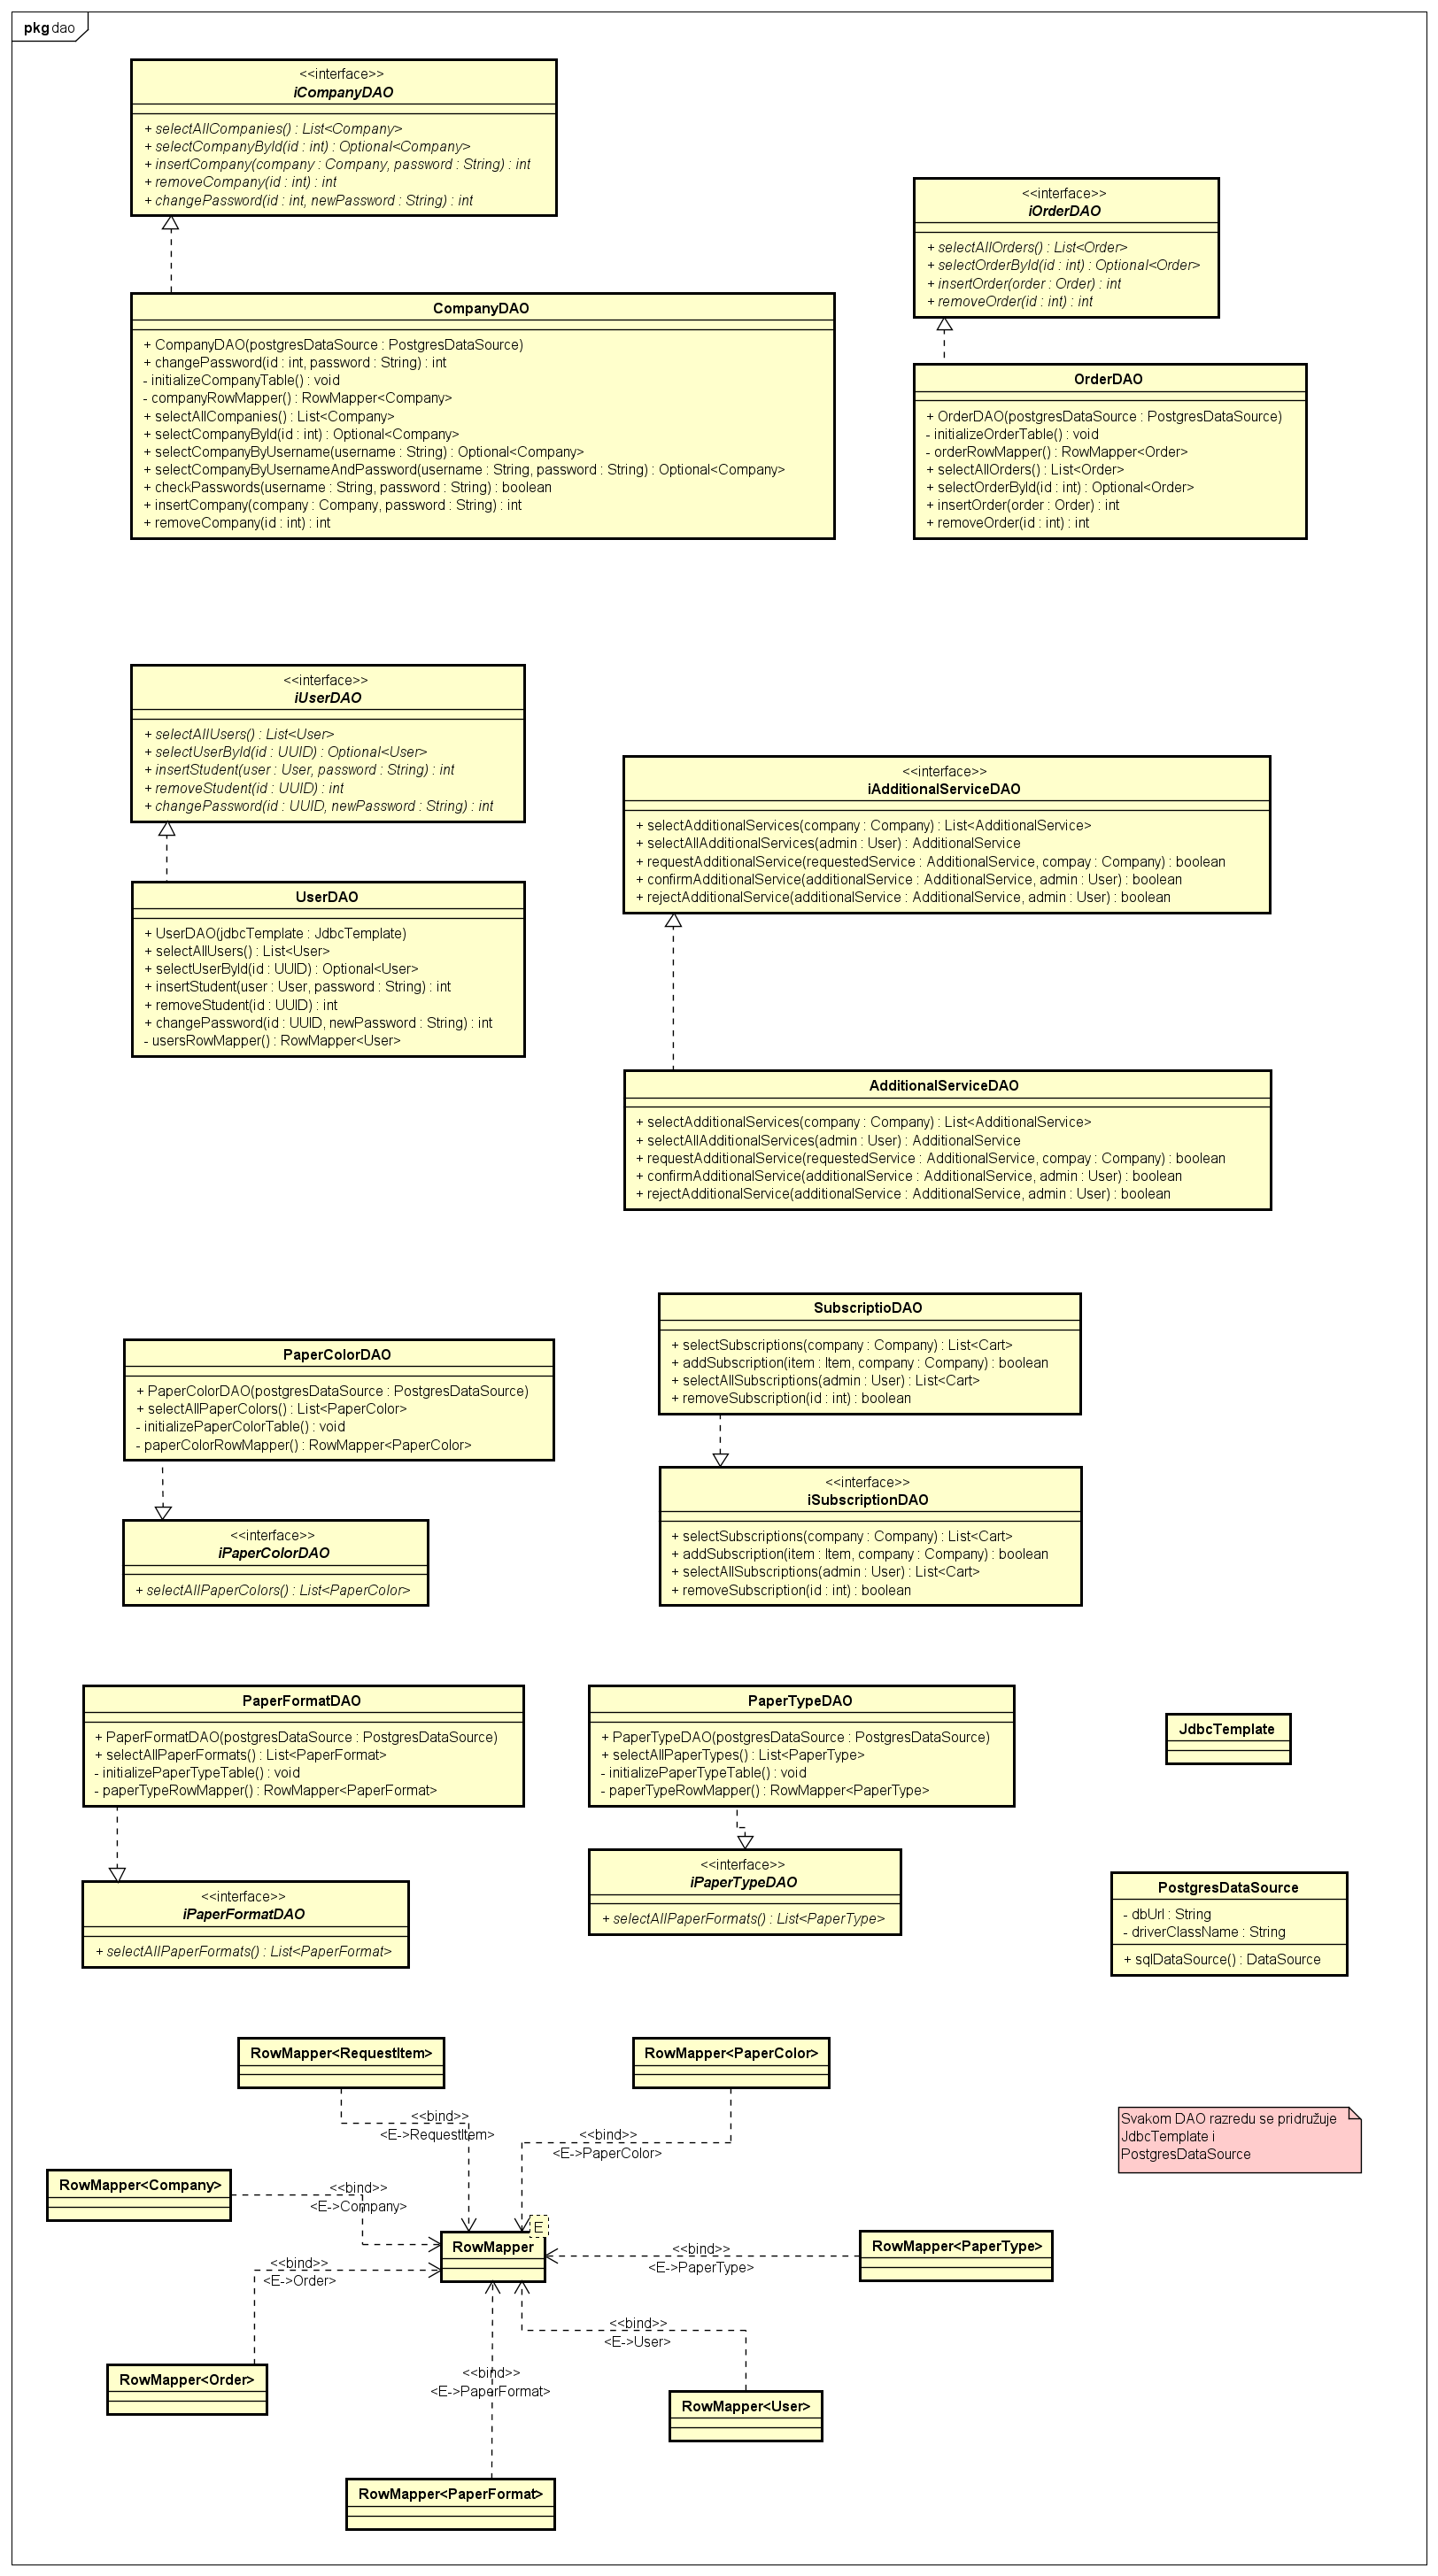
\includegraphics[scale=0.29]{dijagrami/dij_raz_dao_ureden.PNG} 
				\centering
				\caption{Dijagram razreda - DAO-i}
				\label{fig:dij_raz3}%label mora biti drugaciji za svaku sliku
			\end{figure}
		
			\begin{figure}[H]
				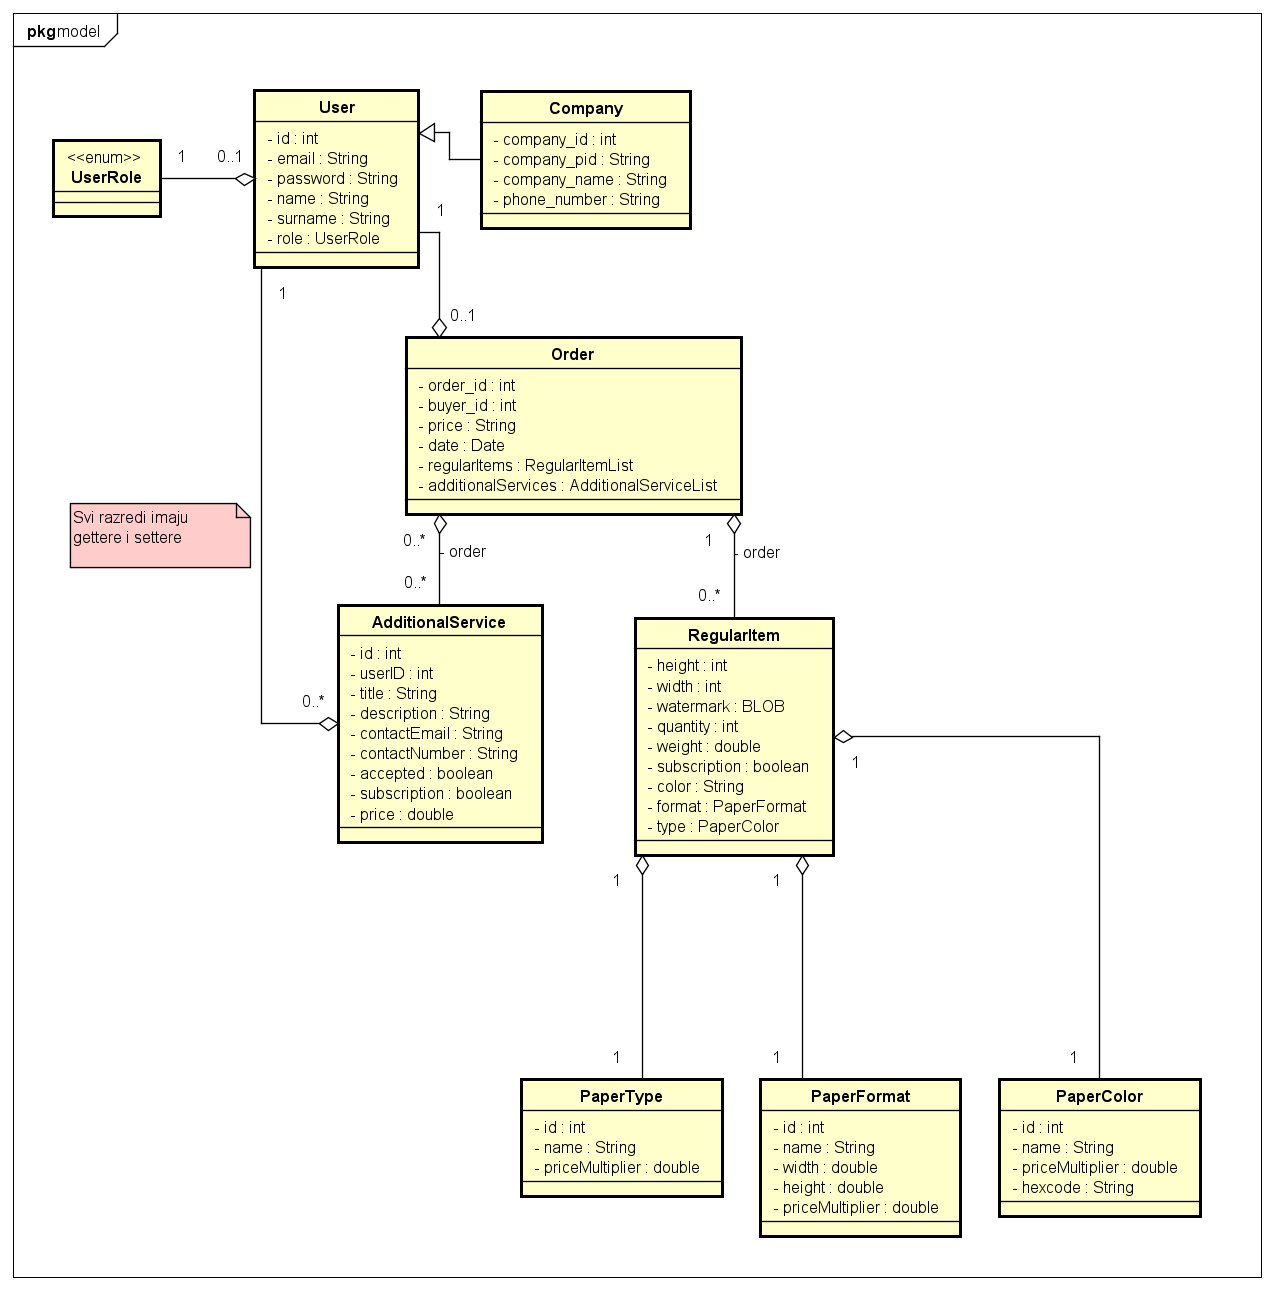
\includegraphics[scale=0.4]{dijagrami/dij_raz_model.PNG} 
				\centering
				\caption{Dijagram razreda - modeli}
				\label{fig:dij_raz4}%label mora biti drugaciji za svaku sliku
			\end{figure}
			
			\eject
		
		\section{Dijagram stanja}
			Dijagram stanja prikazuje stanja objekta te prijelaze iz jednog stanja u drugo temeljene na događajima. Na slici je prikazan dijagram stanja za poslovnog korisnika, registriranog ili ne. Nakon prijave ili registracije, klijentu se odmah prikazuje stranica "Narudžbe" na kojoj može vidjeti svoje dosadašnje narudžbe, stvoriti nove te ih dodati u košaricu. U svakom trenutku klijent se može pozicionirati u svoj "Profil", u "Zahtjeve" ili u navedene "Narudžbe" i "Košaricu". Ukoliko se pozicionira u "Zahtjeve", tamo može pregledavati status postojećih zahtjeva ili stvoriti novi zahtjev klikom na "Novi zahtjev", te iste može dodati u košaricu klikom na ikonicu košarice što ga ponovo prebacuje na "Košaricu". Ukoliko se pozicionira u "Profil", od tamo može pristupiti svojim pretplatama klikom na "Popis pretplata", gdje ih zatim može dodavati i brisati. Iz "Profila" se također može odjaviti što ga prebacuje na početnu stranicu "Prijave".
			\\
			\begin{figure}[H]
				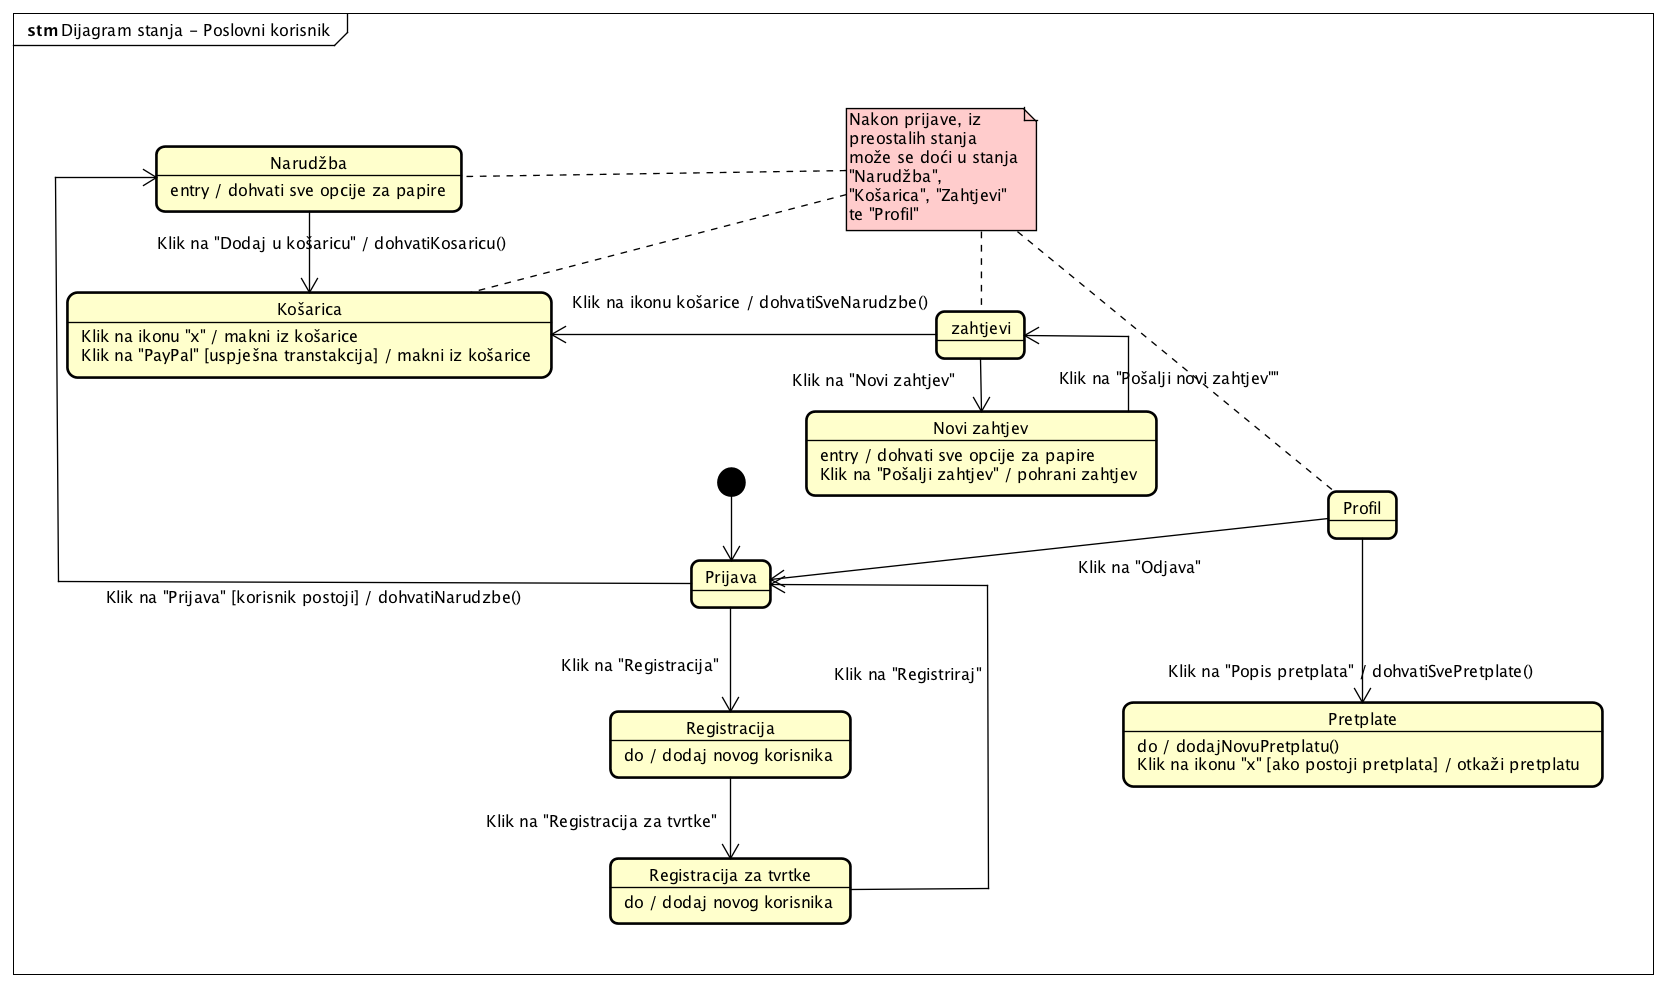
\includegraphics[scale=0.4]{dijagrami/dij_stanja.PNG} 
				\centering
				\caption{Dijagram stanja}
				\label{fig:dij_stanja}%label mora biti drugaciji za svaku sliku
			\end{figure}
			%\textbf{\textit{dio 2. revizije}}\\
			
		%	\textit{Potrebno je priložiti dijagram stanja i opisati ga. Dovoljan je jedan dijagram stanja koji prikazuje \textbf{značajan dio funkcionalnosti} sustava. Na primjer, stanja korisničkog sučelja i tijek korištenja neke ključne funkcionalnosti jesu značajan dio sustava, a registracija i prijava nisu. }
			
			
			\eject 
		
		\section{Dijagram aktivnosti}
			
			%\textbf{\textit{dio 2. revizije}}\\
			
			 
			 Dijagram aktivnosti koristi se za prikaz poslovnih procesa te upravljačkog i podatkovnog toka. On je prigodan za opis sinkronizacije i konkurentnosti, no ne i za modeliranje događajima poticanog ponašanja.
			 \\
			 Sljedeći dijagram prikazuje proces kreiranja narudžbe u slučaju privatnog korisnika. Korisnik se prijavi u sustav, odabire što želi naručiti te potom, nakon što izabere sve što mu je potrebno, odabire pregled košarice i plaća narudžbu te se ona naplaćuje.
			 \\
			 \begin{figure}[H]
			 	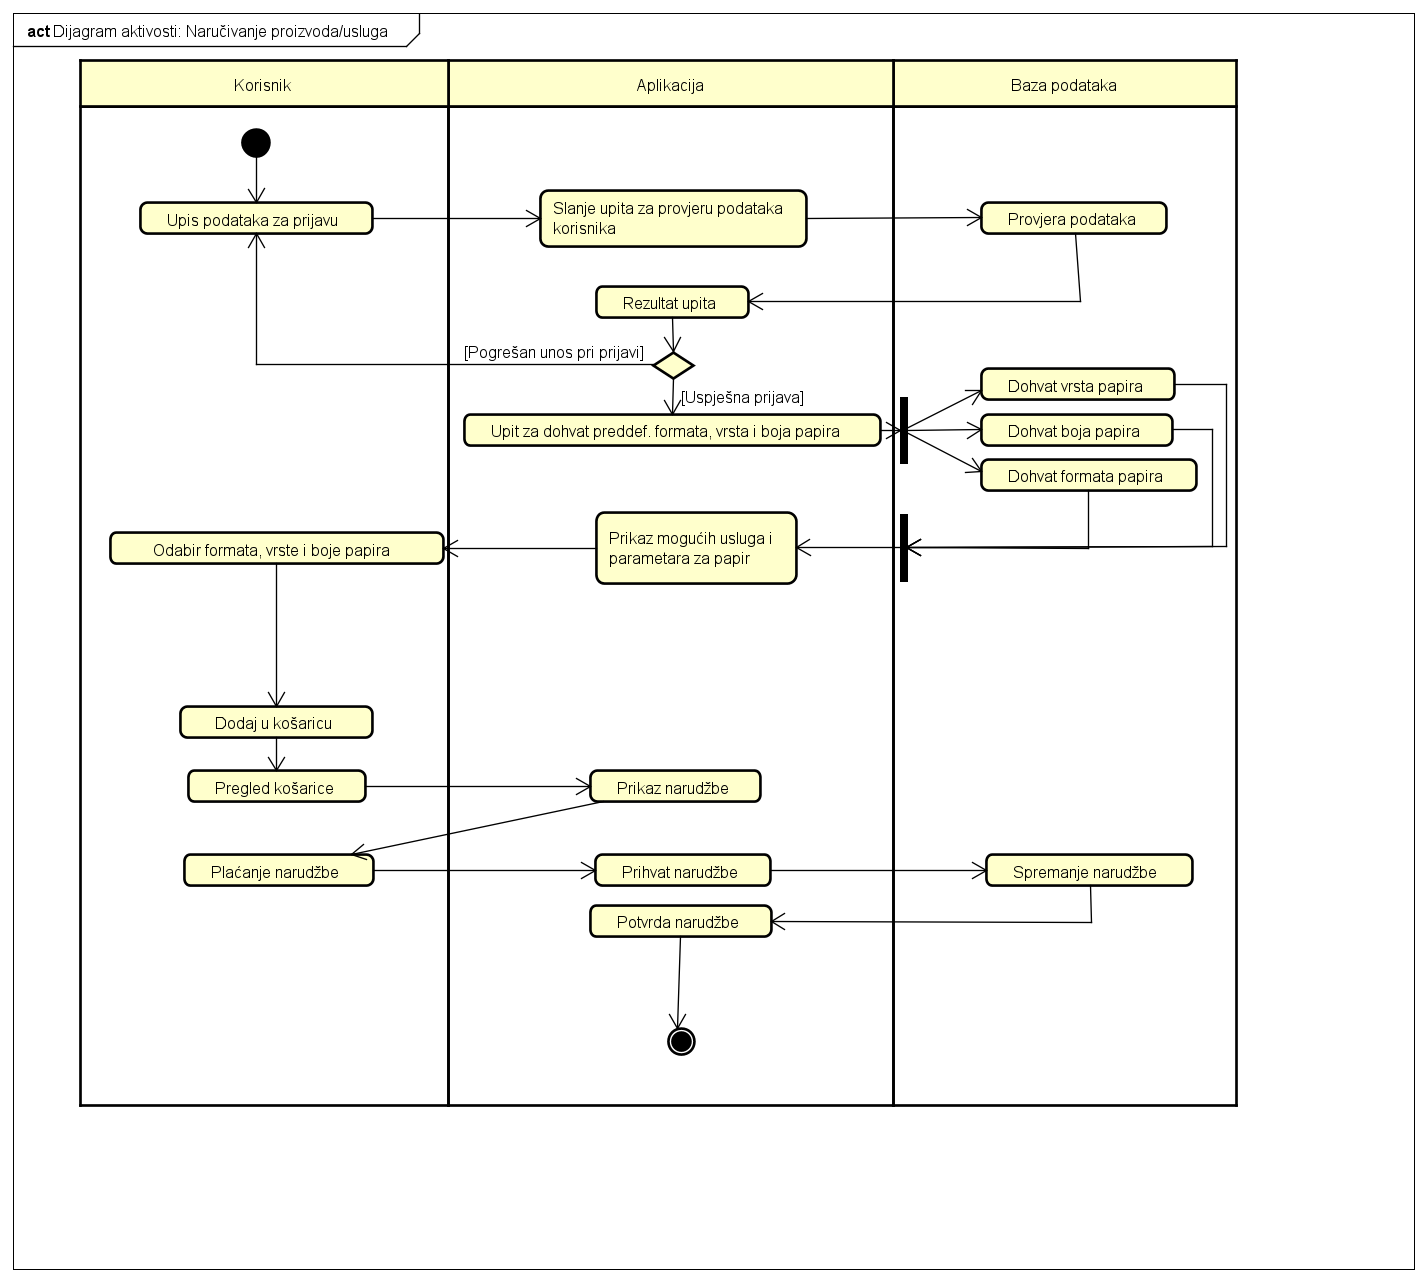
\includegraphics[scale=0.5]{dijagrami/dijagram_aktivnosti.PNG} 
			 	\centering
			 	\caption{Dijagram aktivnosti}
			 	\label{fig:dij_akt}%label mora biti drugaciji za svaku sliku
			 \end{figure}
			
			
			
			\eject
		\section{Dijagram komponenti}
			Dijagram komponenti prikazan na slici  opisuje organizaciju i međuovisnost
			komponenti, interne strukture i odnose prema okolini. Sustavu se pristupa preko sučelja. Klijent pristupa web aplikaciji koristeći web preglednik i sučelje REST API. Web aplikacija organizirana je modularno prema pravilima radnog okvira Java Spring Boota. Modul DAO je zadužen za dohvat i obradu podatka iz baze preko sučelja SQL API te povezivanje istih s Modelom predstavlja klase sustava.  Modul Service zatim te podatke obraduje na aplikaciji svojstven način, a modul Controllers je zadužen za komunikaciju HTTPS protokolom sa Klijentom.
			
			\begin{figure}[H]
				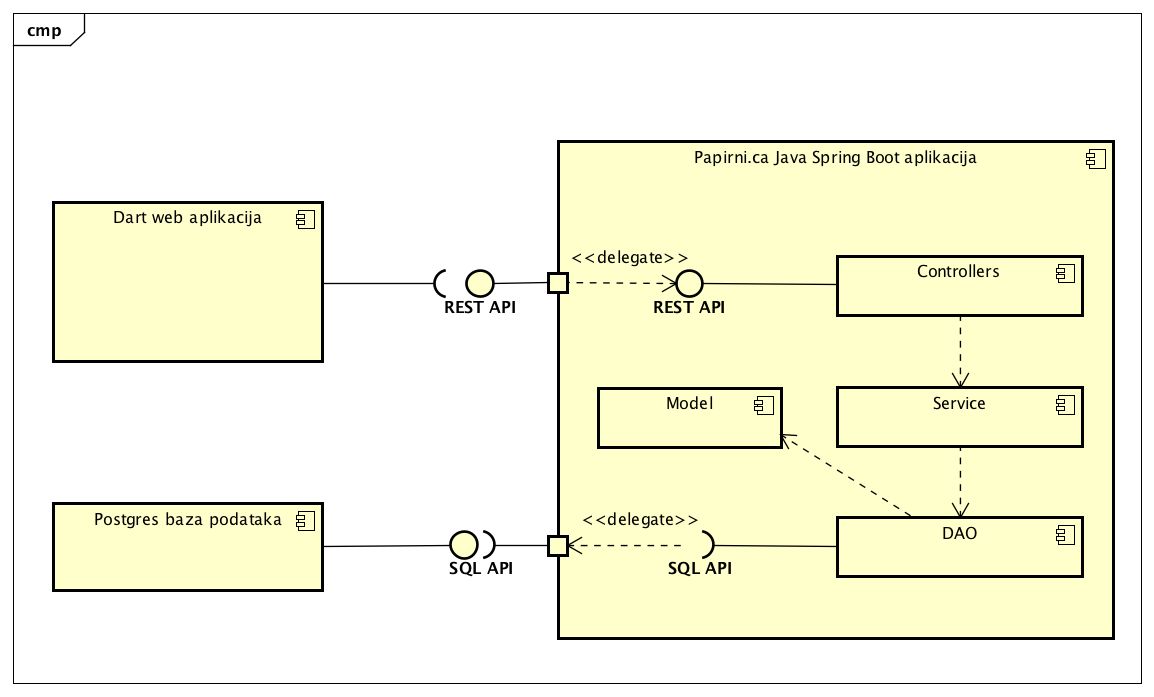
\includegraphics[scale=0.55]{dijagrami/dij_komp.PNG} 
				\centering
				\caption{Dijagram komponenti}
				\label{fig:dij_komp}%label mora biti drugaciji za svaku sliku
			\end{figure}
			%\textbf{\textit{dio 2. revizije}}\\
		
		%	 \textit{Potrebno je priložiti dijagram komponenti s pripadajućim opisom. Dijagram komponenti treba prikazivati strukturu cijele aplikacije.}
	\chapter{Implementacija i korisničko sučelje}
		
		
		\section{Korištene tehnologije i alati}
		
			%\textbf{\textit{dio 2. revizije}}
			
			 %\textit{Detaljno navesti sve tehnologije i alate koji su primijenjeni pri izradi dokumentacije i aplikacije. Ukratko ih opisati, te navesti njihovo značenje i mjesto primjene. Za svaki navedeni alat i tehnologiju je potrebno \textbf{navesti internet poveznicu} gdje se mogu preuzeti ili više saznati o njima}.
			 
			 \normalsize{Komunikacija među članovima tima najvećim je dijelom ostvarena putem platforme  \underline{Discord},\footnote{https://discord.com/} dok su pojedini kraći sastanci nakon konzultacija/demonstracija održani na platformi \underline{MS Teams}.\footnote{https://www.microsoft.com/hr-hr/microsoft-365/microsoft-teams/group-chat-software/}
			 	
			 Za dizajn izgleda aplikacije korišten je software \underline{Adobe XD},\footnote{https://www.adobe.com/products/xd.html}
			 a za izradu UML dijagrama \underline{Astah}.\footnote{https://astah.net/}
			 \underline{Git}\footnote{https://git-scm.com/} je služio kao sustav za upravljanje izvornim kodom na projektu čiji je udaljeni repozitorij smješten na web platformi \underline{GitLab}.\footnote{https://about.gitlab.com/}
			 \newline Uređivanje dokumentacije odvijalo se u okruženju \underline{TeXstudio},\footnote{https://www.texstudio.org/} a jedan od uređivača za pisanje programa za samu aplikaciju bio je \underline{Visual Studio Code}.\footnote{https://code.visualstudio.com/}
			 
			 Za razvoj \textit{frontenda} korišteni su \underline{Dart}\footnote{https://dart.dev/} i \underline{Flutter}.\footnote{https://flutter.dev/} 
			 Dart je programski jezik optimiziran za izgradnju UI-a s posebnim dodatcima kao što su \textit{spread operator} i \textit{collection if} koji omogućavaju lakšu prilagodbu UI-a nekoj platformi, pritom imajući poznatu sintaksu koju je lako svladati. Flutter je Google-ov UI alat za programiranje u Dartu koji se hvali mogućnošću brzog razvoja iznimno vizualno privlačnih aplikacija koje mogu biti mobilne, web ili desktop.
			 
			 Za razvoj \textit{backenda} korišten je \underline{Java Spring \textit{framework}}\footnote{https://spring.io/} (radni okvir). Spring je brz, fleksibilan i siguran okvir za rad s DAO, a poznat je po MVC obrascu korištenjem anotacija.
			 
			 Baza podataka je relacijska baza podataka napravljena putem \underline{PostgreSQL}\footnote{https://www.postgresql.org/}. To je sistem baze podataka s kojim smo upoznati tijekom studija na FER-u, a poznat je po dobrim performansama, pouzdanosti i robusnim značajkama.
			 
			 \underline{Heroku}\footnote{https://www.heroku.com/} je korišten za puštanje aplikacije u pogon. Heroku je \textit{cloud Platform as a Service (PaaS)} koji se bazira na kontejnerima. Podržava mnoštvo programskih jezika i omogućuje integraciju s GitLabom. \textit{PaaS} je platforma koja omogućuje razvoj, pokretanje i upravljanje aplikacijama uz zaobilaženje kompleksnosti koju donosi izrada infrastrukture tipično povezane s izgradnjom aplikacije. Time je povećana učinkovitost i olakšano održavanje i unaprjeđenje aplikacije.
		 }
			
			
			\eject 
		
	
		\section{Ispitivanje programskog rješenja}
			
			%\textbf{\textit{dio 2. revizije}}\\
			
			% \textit{U ovom poglavlju je potrebno opisati provedbu ispitivanja implementiranih funkcionalnosti na razini komponenti i na razini cijelog sustava s prikazom odabranih ispitnih slučajeva. Studenti trebaju ispitati temeljnu funkcionalnost i rubne uvjete.}
			\textit {Nisu provedeni svi traženi testovi.}
			
			\subsection{Ispitivanje komponenti}
		%	\textit{Potrebno je provesti ispitivanje jedinica (engl. unit testing) nad razredima koji implementiraju temeljne funkcionalnosti. Razraditi \textbf{minimalno 6 ispitnih slučajeva} u kojima će se ispitati redovni slučajevi, rubni uvjeti te izazivanje pogreške (engl. exception throwing). Poželjno je stvoriti i ispitni slučaj koji koristi funkcionalnosti koje nisu implementirane. Potrebno je priložiti izvorni kôd svih ispitnih slučajeva te prikaz rezultata izvođenja ispita u razvojnom okruženju (prolaz/pad ispita). }
			Komponente su ispitane sljedećim unit testovima. 
			\begin{figure}[H]
				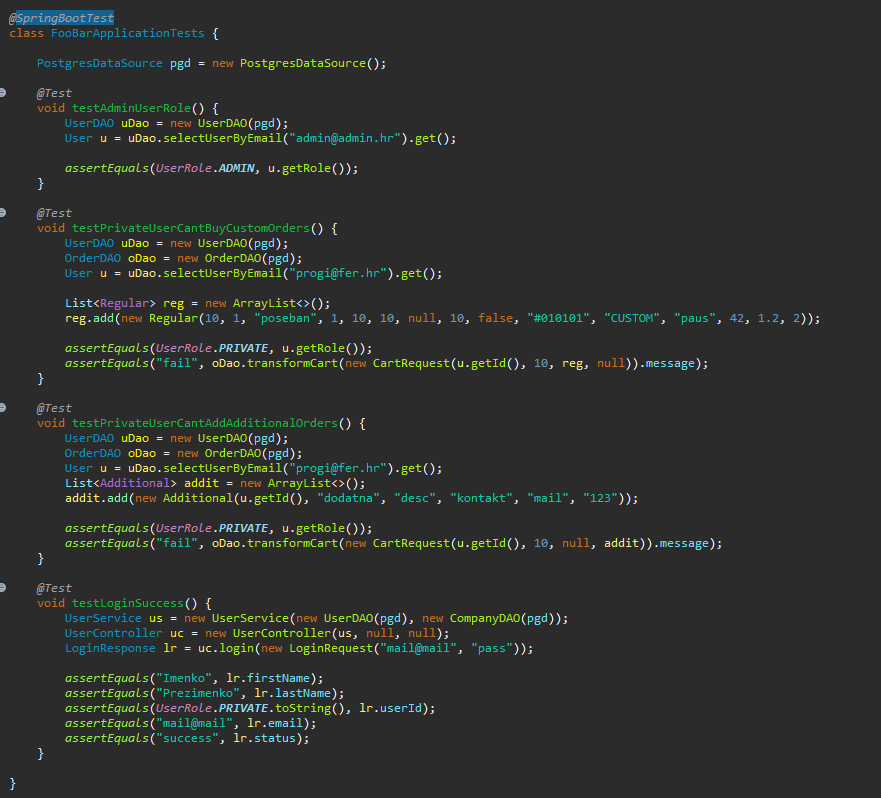
\includegraphics[scale=0.5]{slike/testovi.PNG} 
				\centering
				\caption{Unit testovi}
				\label{fig:unit}%label mora biti drugaciji za svaku sliku
			\end{figure}
			
			\subsection{Ispitivanje sustava}
			
			% \textit{Potrebno je provesti i opisati ispitivanje sustava koristeći radni okvir Selenium\footnote{\url{https://www.seleniumhq.org/}}. Razraditi \textbf{minimalno 4 ispitna slučaja} u kojima će se ispitati redovni slučajevi, rubni uvjeti te poziv funkcionalnosti koja nije implementirana/izaziva pogrešku kako bi se vidjelo na koji način sustav reagira kada nešto nije u potpunosti ostvareno. Ispitni slučaj se treba sastojati od ulaza (npr. korisničko ime i lozinka), očekivanog izlaza ili rezultata, koraka ispitivanja i dobivenog izlaza ili rezultata.\\ }
			 
			 %\textit{Izradu ispitnih slučajeva pomoću radnog okvira Selenium moguće je provesti pomoću jednog od sljedeća dva alata:}
			 %\begin{itemize}
			 	%\item \textit{dodatak za preglednik \textbf{Selenium IDE} - snimanje korisnikovih akcija radi automatskog ponavljanja ispita	}
			 	%\item \textit{\textbf{Selenium WebDriver} - podrška za pisanje ispita u jezicima Java, C\#, PHP koristeći posebno programsko sučelje.}
			 %\end{itemize}
		 	%\textit{Detalji o korištenju alata Selenium bit će prikazani na posebnom predavanju tijekom semestra.}
			
			\eject 
		
		
		\section{Dijagram razmještaja}
			
		%	\textbf{\textit{dio 2. revizije}}
			
			% \textit{Potrebno je umetnuti \textbf{specifikacijski} dijagram razmještaja i opisati ga. Moguće je umjesto specifikacijskog dijagrama razmještaja umetnuti dijagram razmještaja instanci, pod uvjetom da taj dijagram bolje opisuje neki važniji dio sustava.}
			Dijagram razmještaja pruža uvid u topologiju sklopovlja i programsku potporu koja se
			koristi u implementaciji sustava. Klijenti koriste mobilnu aplikaciju kako bi pristupili samoj aplikaciji. Komunikacija između klijenta i poslužitelja bazira se na HTTPS protokolu dok se na poslužiteljskom 
			računalu nalaze web poslužitelj i poslužitelj baze podataka.
			\\
			 \begin{figure}[H]				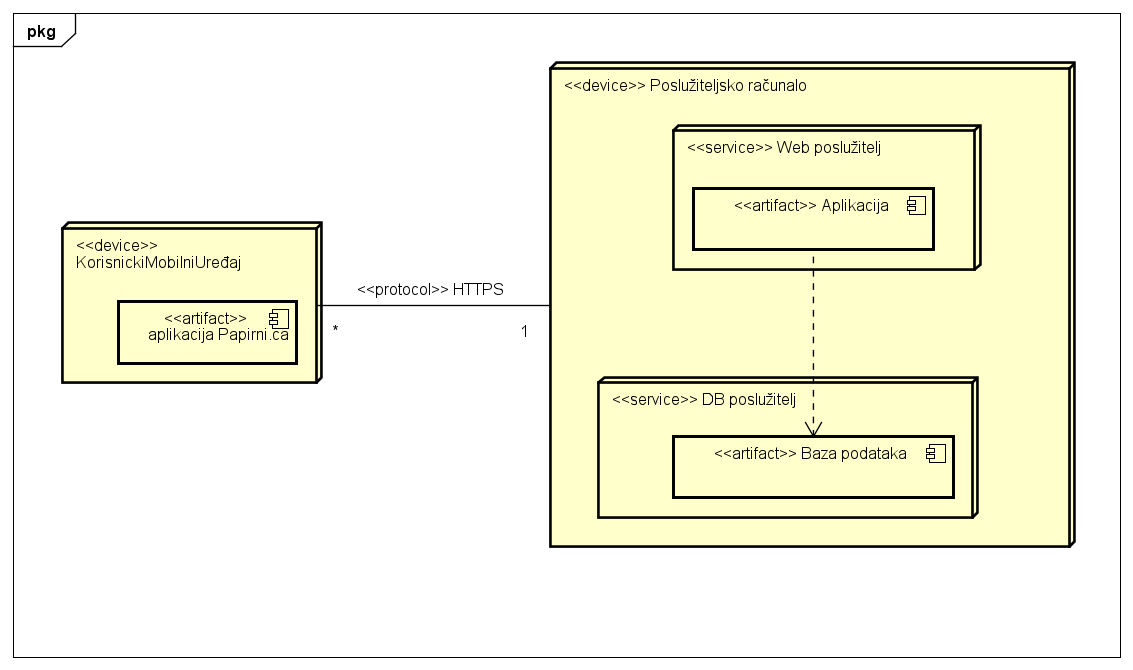
\includegraphics[scale=0.55]{dijagrami/dij_razmjestaj.PNG} 
				\centering
				\caption{Dijagram razmještaja}
				\label{fig:dij_ramjestaj}%label mora biti drugaciji za svaku sliku
			\end{figure}
			
			\eject 
		
		\section{Upute za puštanje u pogon}
			
			\vspace{5mm}
			\noindent \textbf{Izrada Heroku profila}\newline
			Potrebno je napraviti profil na službenim stranicama Herokua.
			
			\vspace{5mm}
			\noindent \textbf{Instalacija Heroku CLI-a}\newline
			Sljedeći korak je sa službene stranice Herokua skinuti Heroku CLI i provesti klasičnu instalaciju.
			
			\vspace{5mm}
			\noindent \textbf{Namještanje i stvaranje Heroku aplikacije}\newline
			Zatim je potrebno otvoriti komandnu liniju i pozicionirati se u direktorij u kojemu će se nalaziti željeni projekt. Pokrenuti naredbu "heroku login" te na upit za otvaranje preglednika kako bi se proveo login stisnuti "q" ako ne 
			želite provesti registraciju, a ako želite stisnite bilo koju preostalu tipku na tipkovnicu. U potvrdnom slučaju se otvara preglednik te je nužno stisnuti "Log In" i prijaviti se. Kako bi se aplikacija stvorila potrebno je u komandnu liniju upisati "git init" pa "heroku create" te se nova aplikacija vašeg profila stvara i ispisuje njeno ime.
			\begin{figure}[H]
				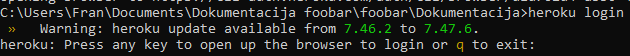
\includegraphics[scale=0.8]{slike/heroku_login.PNG} 
				\centering
				\caption{Upis naredbe za prijavu u Heroku CLI te upit}
				\label{fig:heroku_login}%label mora biti drugaciji za svaku sliku
			\end{figure}
		
			\begin{figure}[H]
				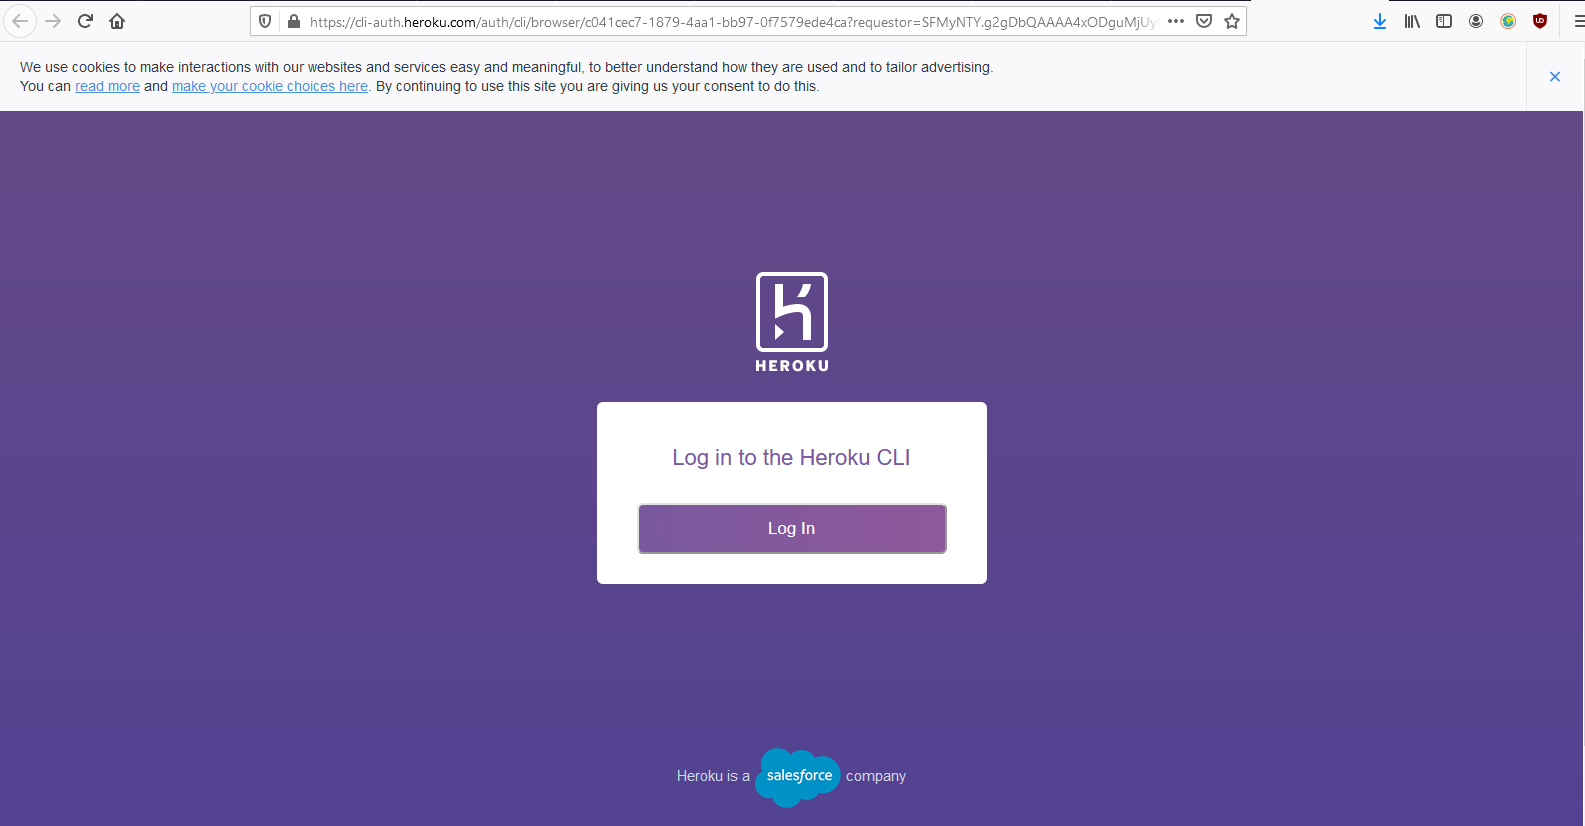
\includegraphics[scale=0.4]{slike/heroku_login_browser.PNG} 
				\centering
				\caption{Otvoreni preglednik za prijavu na Heroku}
				\label{fig:heroku_login_browser}%label mora biti drugaciji za svaku sliku
			\end{figure}
		
			\begin{figure}[H]
				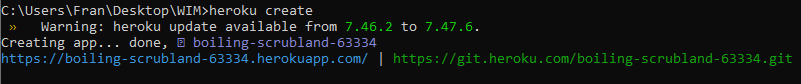
\includegraphics[scale=0.8]{slike/heroku_stvorena_aplikacija.PNG} 
				\centering
				\caption{Naredba za stvaranje nove Heroku aplikacije te ispis dodjeljenog imena}
				\label{fig:heroku_stvorena_aplikacija}%label mora biti drugaciji za svaku sliku
			\end{figure}
			
			\vspace{5mm}
			\noindent \textbf{Namještanje i stvaranje baze podataka na Herokuu}\newline
			Kako bi se stvorila baza podataka u komandnu liniju je potrebno upisati "heroku addons:create heroku-postgresql -a $\langle$APLIKACIJA$\rangle$" gdje je $\langle$APLIKACIJA$\rangle$ ime vaše aplikacije.
			
			\begin{figure}[H]
				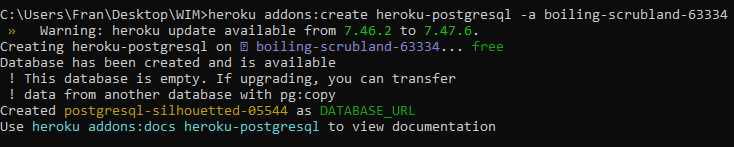
\includegraphics[scale=0.8]{slike/heroku_stvaranje_baze_podataka.PNG} 
				\centering
				\caption{Naredba za stvaranje PostgreSQL baze podataka za Heroku aplikaciju te ispis dodjeljenog imena}
				\label{fig:heroku_stvaranje_baze_podataka}%label mora biti drugaciji za svaku sliku
			\end{figure}
			
			\vspace{5mm}
			 \noindent \textbf{Instalacija PostgreSQL-a}\newline
			 Sa službene stranice je potrebno skinuti i instalirati PostgreSQL i potom staviti PostgreSQL u sistemske varijable.
			 
			 \vspace{5mm}
			 \noindent \textbf{Stvaranje i punjenje baze podataka}\newline
			 Kako bismo imali funkcionalnu bazu podataka potrebno je izmijeniti database\_and\_inserts.sql sa repozitorija tako da promijenimo vrijednosti INSERT naredbe u kojoj se dodaje administrator. Zatim u komandnoj liniji treba pokrenuti "heroku pg:psql -a $\langle$APLIKACIJA$\rangle$" što nas spaja na konzolu baze podataka. Zatim treba jednostavno kopirati i zalijepiti izmijenjeni database\_and\_inserts.sql.
			 
			 \begin{figure}[H]
			 	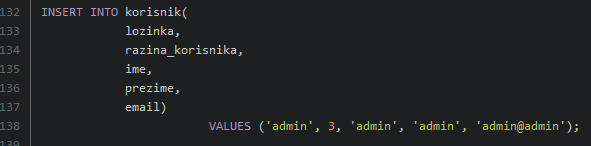
\includegraphics[scale=0.8]{slike/sql_admin.PNG} 
			 	\centering
			 	\caption{Dio SQL upita koji se treba promijeniti u lozinka, 3, ime, prezime i email željenog administratora}
			 	\label{fig:sql_admin}%label mora biti drugaciji za svaku sliku
			 \end{figure}
		 
			 \begin{figure}[H]
			 	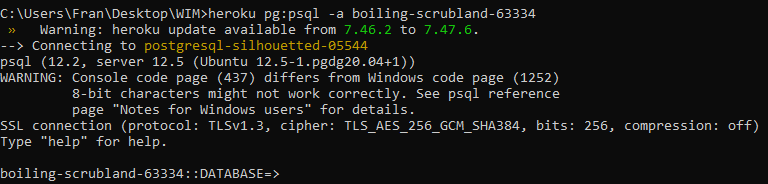
\includegraphics[scale=0.8]{slike/baza_spajanje.PNG} 
			 	\centering
			 	\caption{Naredba za spajanje na stvorenu bazu podataka}
			 	\label{fig:baza_spajanje}%label mora biti drugaciji za svaku sliku
			 \end{figure}
			 
			 \vspace{5mm}
			 \noindent \textbf{Stavljanje backenda na Heroku}\newline
			 Potrebno je skinuti izvorni kod iz direktorija fooBarServer sa repozitorija i staviti ga u direktorij u kojemu smo stvorili Heroku aplikaciju. Zatim treba, pomoću redom "git add .", "git commit -m "$\langle$VASA\_PORUKA$\rangle$"" i  "git push origin master", aplikaciju postaviti na server. To pokreće izgradnju aplikacije te je nakon toga aplikacija spremna za korištenje.
			 
			 \begin{figure}[H]
			 	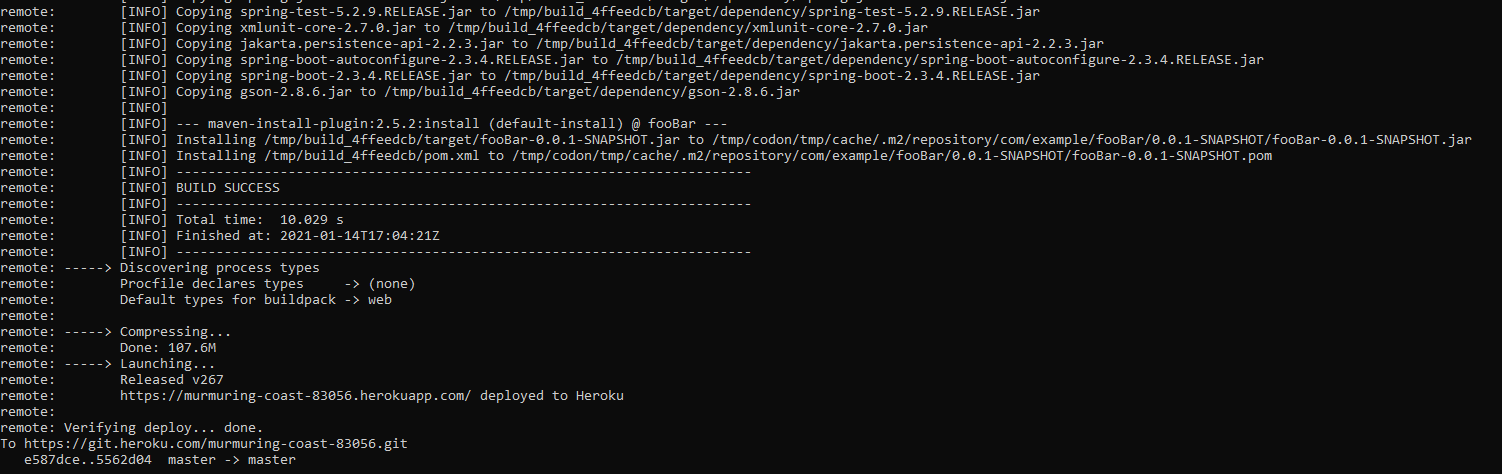
\includegraphics[scale=0.4]{slike/izgradnja_gotova.PNG} 
			 	\centering
			 	\caption{Poruka da se baze uspješno postavila na Heroku}
			 	\label{fig:izgradnja_gotova}%label mora biti drugaciji za svaku sliku
			 \end{figure}
			 
			 \vspace{5mm}
			 \noindent \textbf{Pokretanje mobilne aplikacije} \newline
			 Potrebno je iz direktorija "Izvrsni kod/apk" skinuti aplikacije za mobitel te instalirati onu za Vaš mobilni uređaj. Klikom na ikonu aplikacije Papirni.ca moguće je započeti njeno korištenje.
			 
			\eject 
	\chapter{Zaključak i budući rad}
		
	%	\textbf{\textit{dio 2. revizije}}\\
		
		 %\textit{U ovom poglavlju potrebno je napisati osvrt na vrijeme izrade projektnog zadatka, koji su tehnički izazovi prepoznati, jesu li riješeni ili kako bi mogli biti riješeni, koja su znanja stečena pri izradi projekta, koja bi znanja bila posebno potrebna za brže i kvalitetnije ostvarenje projekta i koje bi bile perspektive za nastavak rada u projektnoj grupi.}
		
		% \textit{Potrebno je točno popisati funkcionalnosti koje nisu implementirane u ostvarenoj aplikaciji.}
		\normalsize
		Projekt \textit{Papirni.ca} bio je u izradi 4.10.2020. - 14.1.2021. Tijekom tih 14 tjedana tim je izradio aplikaciju s (gotovo svim) traženim funkcionalnostima.
		Zadatak je bio dizajnirati, programirati i isporučiti aplikaciju koja predstavlja papirnicu tj. trgovinu papirom i nekim vezanim uslugama. Korisnici (kupci) podijeljeni su na 2 vrste - privatni i poslovni te ovisno o vrsti kupca mogli su birati između kupovanja papira preddefiniranih i posebnih stilova te pretplaćivati se na proizvode iz papirnice. Plaćanje se trebalo odvijati putem usluga \textit{PayPal} no zbog manjka vremena za taj dio i problema pri implementaciji te funkcionalnosti on nije napravljen (umjesto mjesečnog naplaćivanja, pretplatnike se obavještava o izvršenoj pretplati svaki mjesec).
		\\
		\\
		U prvoj fazi projekta radilo se na okupljanju tima, podijeli posla, dizajnu aplikacije i izradi osnovnih funkcionalnosti. tim je podijeljen na 3 glavne skupine: frontend, backend i miješani poddtim (manji zadaci na frontendu i backendu, dokumentacija). Najprije su osmišljeni izvedba baze podataka i izgled aplikacije. U dokumentaciji su napravljeni prvi osnovni koraci i izrađeni početni dijagrami koji su pomogli u kasnijoj implementaciji funkcionalnosti - obrasci uporabe, sekvencijski dijagrami, model baze
		podataka i dijagram razreda. Tijekom prve faze tim se povremeno sastajao kako bi se razmijenile daljnje ideje i definirali pojedinačni zadaci.  Najveći izazovi u ovoj fazi bili su postavljanje servera i baze podataka na Heroku te uspostavljanje komunikacije između frontenda i backenda koji su razriješeni uz pomoć literature, dokumentacije i već stečenih znanja.
		\\
		\\
		U drugoj fazi projekta radilo se na implementaciji ostatka funkcionalnosti i dovršavanju dokumentacije. Ažurirani su dijagrami iz prethodnih faza (dijagram baze podataka, dijagram razred) uslijed manjih promjena u bazi i nekim razredima. Najveći izazovi u ovoj fazi bili su izrada košarice (cart) i (kasnije) \textit{PayPal}. Backend i frontend timovi imali su regularne tjedne sastanke u ovom periodu na kojemu su osim rasprava zajedno radili na programskom kodu i testirali dobivena rješenja.
		\\
		\\
		Moguće proširenje aplikacije bilo bi uspješno dodavanje usluge \textit{PayPal} i proširenje asortimana papirnice.
		\\
		\\
		Rad na projektu je bilo vrijedno iskustvo i lekcija o zajedničkom radu, organizaciji i usklađenju poddtimova te komunikacije među istima. Proširili smo obzore i stekli nova znanja vezana uz programiranje i rad u sustavu Git koji su zasigurno veliki bonusi za buduće radno okruženje (za koje postoji velika mogućnost da će biti organizirano na sličan način).
		\eject 
	\chapter*{Popis literature}
		\addcontentsline{toc}{chapter}{Popis literature}
	 
		\begin{enumerate}
			
			
			\item  Programsko inženjerstvo, FER ZEMRIS, \url{http://www.fer.hr/predmet/proinz}
			
			\item  I. Sommerville, "Software engineering", 8th ed, Addison Wesley, 2007.
			
			\item  T.C.Lethbridge, R.Langaniere, "Object-Oriented Software Engineering", 2nd ed. McGraw-Hill, 2005.
			
			\item  I. Marsic, Software engineering book``, Department of Electrical and Computer Engineering, Rutgers University, \url{http://www.ece.rutgers.edu/~marsic/books/SE}
			
			\item  The Unified Modeling Language, \url{https://www.uml-diagrams.org/}
			
			\item  Astah Community, \url{http://astah.net/editions/uml-new}
		\end{enumerate}
		
		 
	
	
	\begingroup
	\renewcommand*\listfigurename{Indeks slika i dijagrama}
	%\renewcommand*\listtablename{Indeks tablica}
	%\let\clearpage\relax
	\listoffigures
	%\vspace{10mm}
	%\listoftables
	\endgroup
	\addcontentsline{toc}{chapter}{Indeks slika i dijagrama}


	
	\eject 
		
	\chapter*{Dodatak: Prikaz aktivnosti grupe}
		\addcontentsline{toc}{chapter}{Dodatak: Prikaz aktivnosti grupe}
		
		\section*{Dnevnik sastajanja}
		
		\textbf{\textit{Kontinuirano osvježavanje}}\\
		
	
		
		\begin{packed_enum}
			\item  sastanak
			
			\item[] \begin{packed_item}
				\item Datum: 4. listopada 2020.
				\item Prisustvovali: F. Hrabar, I. Mihovilović, Z. Protulipac, Z. Pećanić, T. Likakur, J. Vujević, M. Kukelšćak
				\item Teme sastanka:
				\begin{packed_item}
					\item  organizacija grupe
					\item  raspodjela posla
				\end{packed_item}
			\end{packed_item}
			
			\item  sastanak
			\item[] \begin{packed_item}
				\item Datum: 15. listopada 2020.
				\item Prisustvovali: F. Hrabar, I. Mihovilović, Z. Protulipac, Z. Pećanić, T. Likakur, J. Vujević, M. Kukelšćak
				\item Teme sastanka:
				\begin{packed_item}
					\item  odabir programske potpore koja će se koristiti
					\item  izgled i dizajn aplikacije
				\end{packed_item}
			\end{packed_item}
			
			\item  sastanak
			\item[] \begin{packed_item}
				\item Datum: 2. 11. 2020.
				\item Prisustvovali: F. Hrabar, I. Mihovilović, Z. Protulipac, Z. Pećanić, T. Likakur, J. Vujević, M. Kukelšćak
				\item Teme sastanka:
				\begin{packed_item}
					\item  izvedba backenda i povezivanje s frontendom (json)
					\item  povezivanje git - Heroku
				\end{packed_item}
			\end{packed_item}
			%
			\item  sastanak
			\item[] \begin{packed_item}
				\item Datum: 8. 11. 2020.
				\item Prisustvovali: F. Hrabar, I. Mihovilović, Z. Protulipac, Z. Pećanić, T. Likakur, J. Vujević, M. Kukelšćak
				\item Teme sastanka:
				\begin{packed_item}
					\item  izvedba frontenda
					\item  json i povezivanje backend-frontend
				\end{packed_item}
			\end{packed_item}
			%
			\item  sastanak
			\item[] \begin{packed_item}
				\item Datum: 20. 11. 2020.
				\item Prisustvovali: F. Hrabar, I. Mihovilović, Z. Protulipac, Z. Pećanić, T. Likakur, J. Vujević, M. Kukelšćak
				\item Teme sastanka:
				\begin{packed_item}
					\item  daljnja podjela posla
					\item  backend
				\end{packed_item}
			\end{packed_item}
			%
			\item  sastanak
			\item[] \begin{packed_item}
				\item Datum: 28. 11. 2020.
				\item Prisustvovali: F. Hrabar, I. Mihovilović, Z. Protulipac, Z. Pećanić, T. Likakur, J. Vujević, M. Kukelšćak
				\item Teme sastanka:
				\begin{packed_item}
					\item  frontend i json
					\item  cart
					\item  dodatci u bazi
					
				\end{packed_item}
			\end{packed_item}
		
			\item  sastanak
			\item[] \begin{packed_item}
				\item Datum: 6. 12. 2020.
				\item Prisustvovali: F. Hrabar, I. Mihovilović, Z. Protulipac, Z. Pećanić, T. Likakur, J. Vujević, M. Kukelšćak
				\item Teme sastanka:
				\begin{packed_item}
					\item  cart
					\item  backend
					\item  podjela posla tijekom praznika
					
					
				\end{packed_item}
			\end{packed_item}
			%
			\item  sastanak
			\item[] \begin{packed_item}
				\item Datum: 12. 12. 2020.
				\item Prisustvovali: F. Hrabar, I. Mihovilović, Z. Protulipac, Z. Pećanić, T. Likakur, J. Vujević, M. Kukelšćak
				\item Teme sastanka:
				\begin{packed_item}
					\item  uloge admina
				
					
				\end{packed_item}
			\end{packed_item}
		
			\item  sastanak
			\item[] \begin{packed_item}
				\item Datum: 18. 12. 2020.
				\item Prisustvovali: F. Hrabar, I. Mihovilović, Z. Protulipac, Z. Pećanić, T. Likakur, J. Vujević, M. Kukelšćak
				\item Teme sastanka:
				\begin{packed_item}
					\item  podjela posla do kraja
					\item dokumentacija - dijagrami u 2. ciklusu
				
					
				\end{packed_item}
			\end{packed_item}
		
			\item  sastanak
			\item[] \begin{packed_item}
				\item Datum: 27. 12. 2020.
				\item Prisustvovali: F. Hrabar, I. Mihovilović, Z. Protulipac, Z. Pećanić, T. Likakur, J. Vujević, M. Kukelšćak
				\item Teme sastanka:
				\begin{packed_item}
					\item  backend
					\item  vodeni žig
				
					
				\end{packed_item}
			\end{packed_item}
		
			\item  sastanak
			\item[] \begin{packed_item}
				\item Datum: 5. 1. 2021.
				\item Prisustvovali: F. Hrabar, I. Mihovilović, Z. Protulipac, Z. Pećanić, T. Likakur, J. Vujević, M. Kukelšćak
				\item Teme sastanka:
				\begin{packed_item}
					\item  završne funkcije
					\item  PayPal
					\item demo alfa inačice - što i kako
					
				\end{packed_item}
			\end{packed_item}
			\item  sastanak
			\item[] \begin{packed_item}
				\item Datum: 12. 1. 2021.
				\item Prisustvovali: F. Hrabar, I. Mihovilović, Z. Protulipac, Z. Pećanić, T. Likakur, J. Vujević, M. Kukelšćak
				\item Teme sastanka:
				\begin{packed_item}
					\item  završavanje i dogovor oko termina kolokviranja
					\item dogovori oko prezentacije
					
				\end{packed_item}
			\end{packed_item}
		
		\end{packed_enum}
	
		
		\eject
		\section*{Tablica aktivnosti}
		

			\begin{longtabu} to \textwidth {|X[7, l]|X[1, c]|X[1, c]|X[1, c]|X[1, c]|X[1, c]|X[1, c]|X[1, c]|}
								
				\cline{2-8} \multicolumn{1}{c|}{\textbf{}} &     \multicolumn{1}{c|}{\rotatebox{90}{\textbf{Fran Hrabar}}} & \multicolumn{1}{c|}{\rotatebox{90}{\textbf{Ivan Mihovilović }}} &	\multicolumn{1}{c|}{\rotatebox{90}{\textbf{Zvonimir Protulipac }}} &
				\multicolumn{1}{c|}{\rotatebox{90}{\textbf{Tomislav Likakur }}} &	\multicolumn{1}{c|}{\rotatebox{90}{\textbf{Zrinka Pećanić }}} &
				\multicolumn{1}{c|}{\rotatebox{90}{\textbf{Josipa Vujević }}} &	\multicolumn{1}{c|}{\rotatebox{90}{\textbf{Mihael Kukelšćak }}} \\ \hline 
				\endfirsthead
				
			
				
			
				\cline{2-8} \multicolumn{1}{c|}{\textbf{}} &     \multicolumn{1}{c|}{\rotatebox{90}{\textbf{Fran Hrabar}}} & \multicolumn{1}{c|}{\rotatebox{90}{\textbf{Ivan Mihovilović }}} &	\multicolumn{1}{c|}{\rotatebox{90}{\textbf{Zvonimir Protulipac }}}&
				\multicolumn{1}{c|}{\rotatebox{90}{\textbf{Tomislav Likakur }}} &	\multicolumn{1}{c|}{\rotatebox{90}{\textbf{Zrinka Pećanić }}} &
				\multicolumn{1}{c|}{\rotatebox{90}{\textbf{Josipa Vujević }}} &	\multicolumn{1}{c|}{\rotatebox{90}{\textbf{Mihael Kukelšćak }}} \\ \hline  
				\endhead
				
				
				\endfoot
							
				 
				\endlastfoot
				
				Upravljanje projektom 		& 10 & 0 & 0 & 0 & 0 & 1 & 0\\ \hline
				Opis projektnog zadatka 	& 0 & 0 & 0 & 0 & 3 & 0 & 0\\ \hline
				
				Funkcionalni zahtjevi       & 2 & 0 & 0 & 0 & 2 & 0 & 0 \\ \hline
				Opis pojedinih obrazaca 	& 5 & 0 & 0 & 0 &  1 & 0 & 1 \\ \hline
				Dijagram obrazaca 			& 0 & 0 & 0 & 0 &  3 & 0 & 0 \\ \hline
				Sekvencijski dijagrami 		& 0 & 0 & 0 & 0 & 2 & 0 & 0 \\ \hline
				Opis ostalih zahtjeva 		& 0 & 0 & 0 & 0 & 1 & 0 & 0 \\ \hline

				Arhitektura i dizajn sustava	 & 1 & 0 & 0 & 0 & 0  & 8 & 1 \\ \hline
				Baza podataka				& 3 & 0 & 2 & 0 & 0 & 1 &  0 \\ \hline
				Dijagram razreda 			& 3 & 0 & 0 & 0 & 2 & 0 &  0 \\ \hline
				Dijagram stanja				& 0 & 0 & 0 & 0 & 0 & 3 & 0 \\ \hline
				Dijagram aktivnosti 		& 0 & 0 & 0 & 0 & 4 & 0 & 0 \\ \hline
				Dijagram komponenti			& 0 & 0 & 0 & 0 & 0 & 3 & 0 \\ \hline
				Korištene tehnologije i alati 		& 0 & 0 & 0 & 0 & 2 & 0 & 0 \\ \hline
				Ispitivanje programskog rješenja 	& 0 & 0 & 2 & 0 & 0 & 0 & 0 \\ \hline
				Dijagram razmještaja			& 0 & 0 & 0 & 0 & 2 & 0 & 0 \\ \hline
				Upute za puštanje u pogon 		& 2 & 0 & 0 & 0 & 0 & 0 & 0 \\ \hline 
				Dnevnik sastajanja 			& 0 & 0 & 0 & 0 & 1 & 0 & 1 \\ \hline
				Zaključak i budući rad 		& 0 & 0 & 0 & 0 & 2 & 0 & 0 \\  \hline
				Popis literature 			& 0 & 0 & 0 & 0 & 1 & 0 & 0 \\  \hline
				 \hline
				Izrada početne stranice 	& 0 & 0 & 0 & 0 & 0 & 1 & 0 \\ \hline 
				Izrada baze podataka 		& 3 & 0 & 8 & 0 & 0 & 0 & 0 \\ \hline 
				Spajanje s bazom podataka 	& 15 & 0 & 15 & 0 & 0 & 0 & 0 \\ \hline
				Back end 					& 15 & 0 & 20 & 0 & 3 & 5 & 15 \\  \hline
				Front end 					& 0 & 35 & 0 & 25 & 0 & 1 & 0 \\  \hline
				Osmišljavanje dizajna 		& 0 & 2 & 0 & 5 & 0 & 1 & 0 \\  \hline
				 							&  &  &  &  &  &  &\\  \hline
			
				%	\caption{\label{tab:referencatablica} Naslov ispod tablice.}	
				
			\end{longtabu}
					
					
		\eject
		\section*{Dijagrami pregleda promjena}
		 Slike stat1 i stat2 prikazuju statistiku za granu master, stat3 za granu devdoc, stat4 za client i stat5 za database.
		 \\
		 \begin{figure}[H]
		 	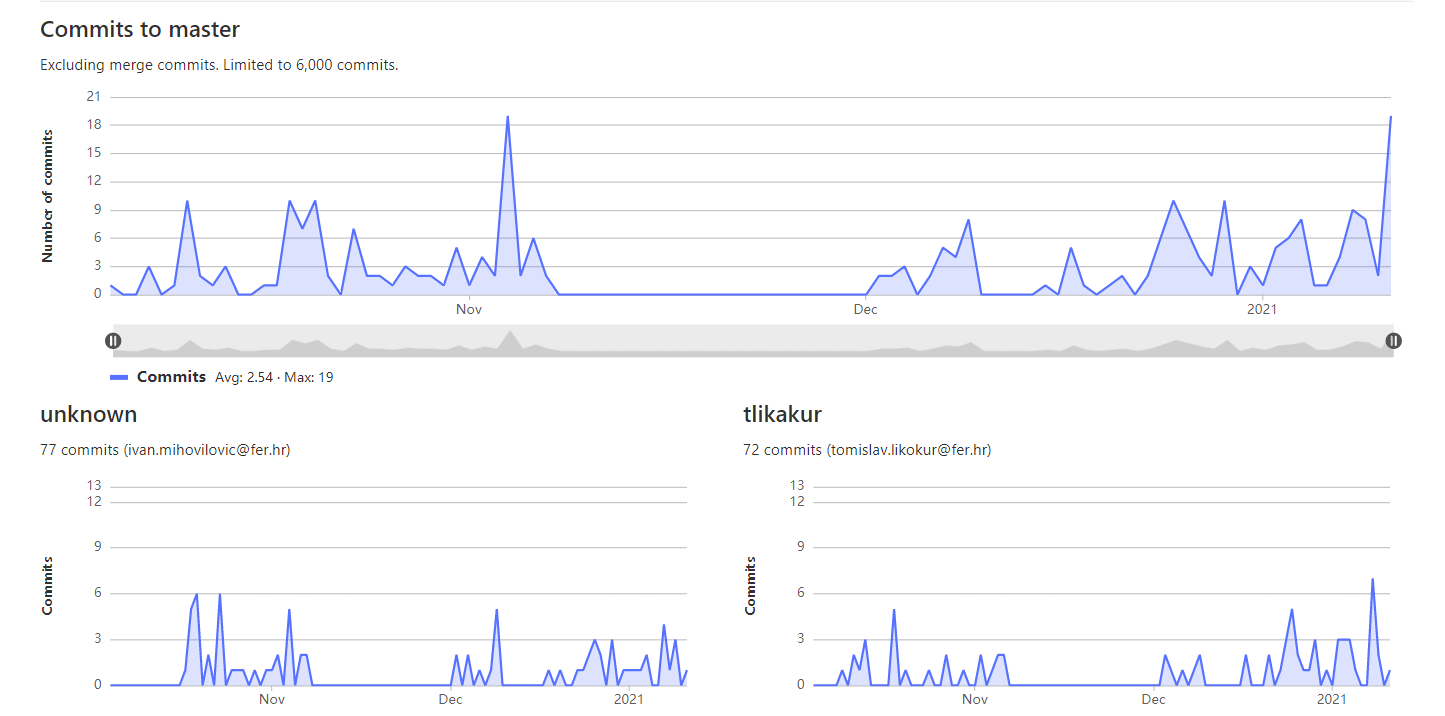
\includegraphics[scale=0.45]{slike/stat1.PNG} 
		 	\centering
		 	\caption{Statistika za granu master}
		 	\label{fig:stat1}%label mora biti drugaciji za svaku sliku
		 \end{figure}
	 	
	 	\begin{figure}[H]
	 		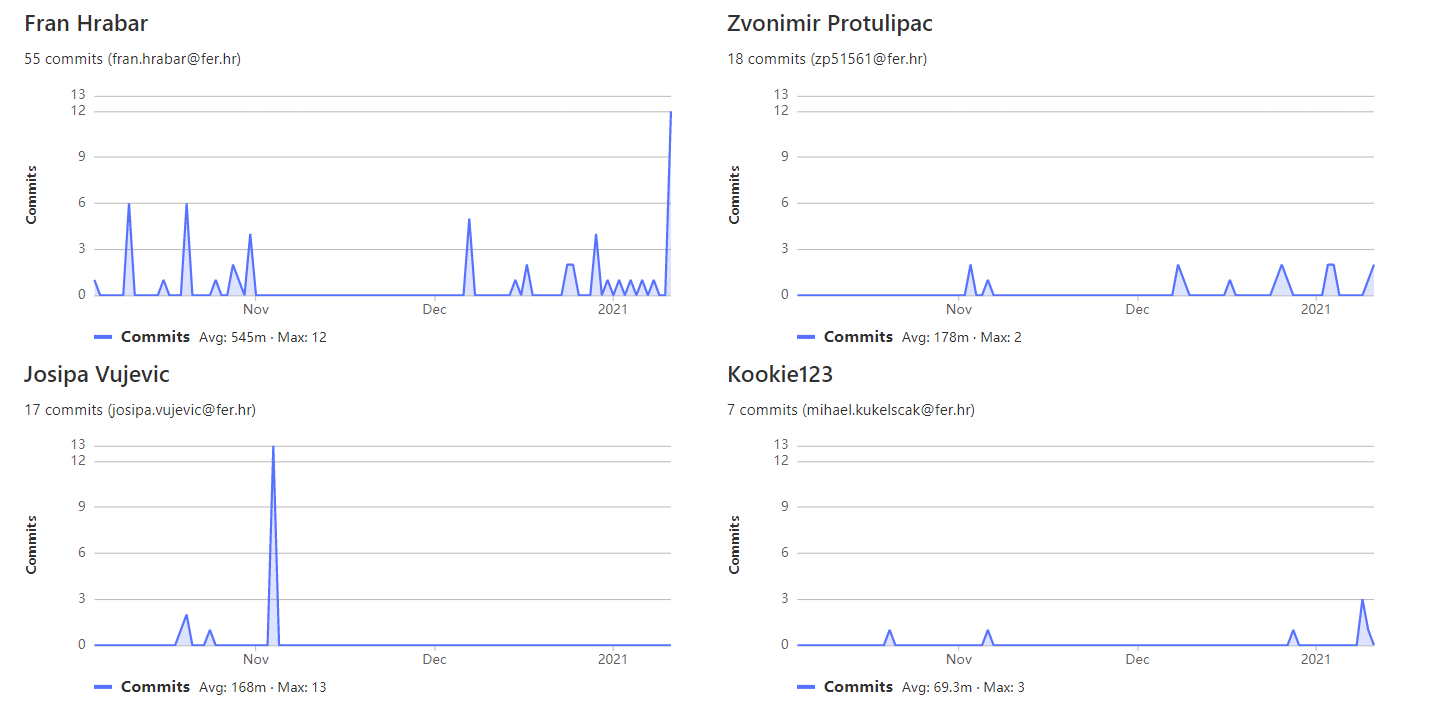
\includegraphics[scale=0.45]{slike/stat2.PNG} 
	 		\centering
	 		\caption{Statistika za granu master - nastavak}
	 		\label{fig:stat2}%label mora biti drugaciji za svaku sliku
	 	\end{figure}
 	
 		\begin{figure}[H]
 			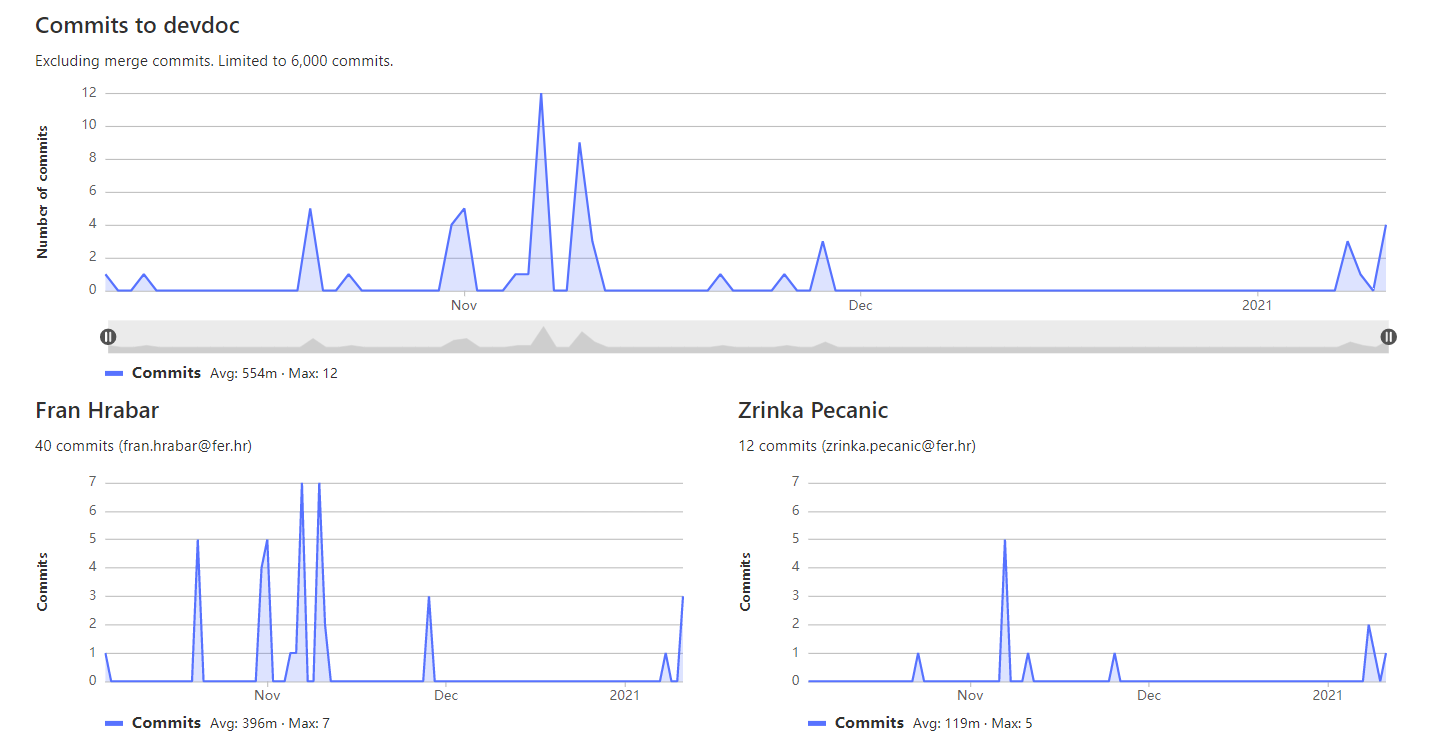
\includegraphics[scale=0.45]{slike/stat3.PNG} 
 			\centering
 			\caption{Statistika za granu devdoc}
 			\label{fig:stat3}%label mora biti drugaciji za svaku sliku
 		\end{figure}
 	
 		\begin{figure}[H]
 			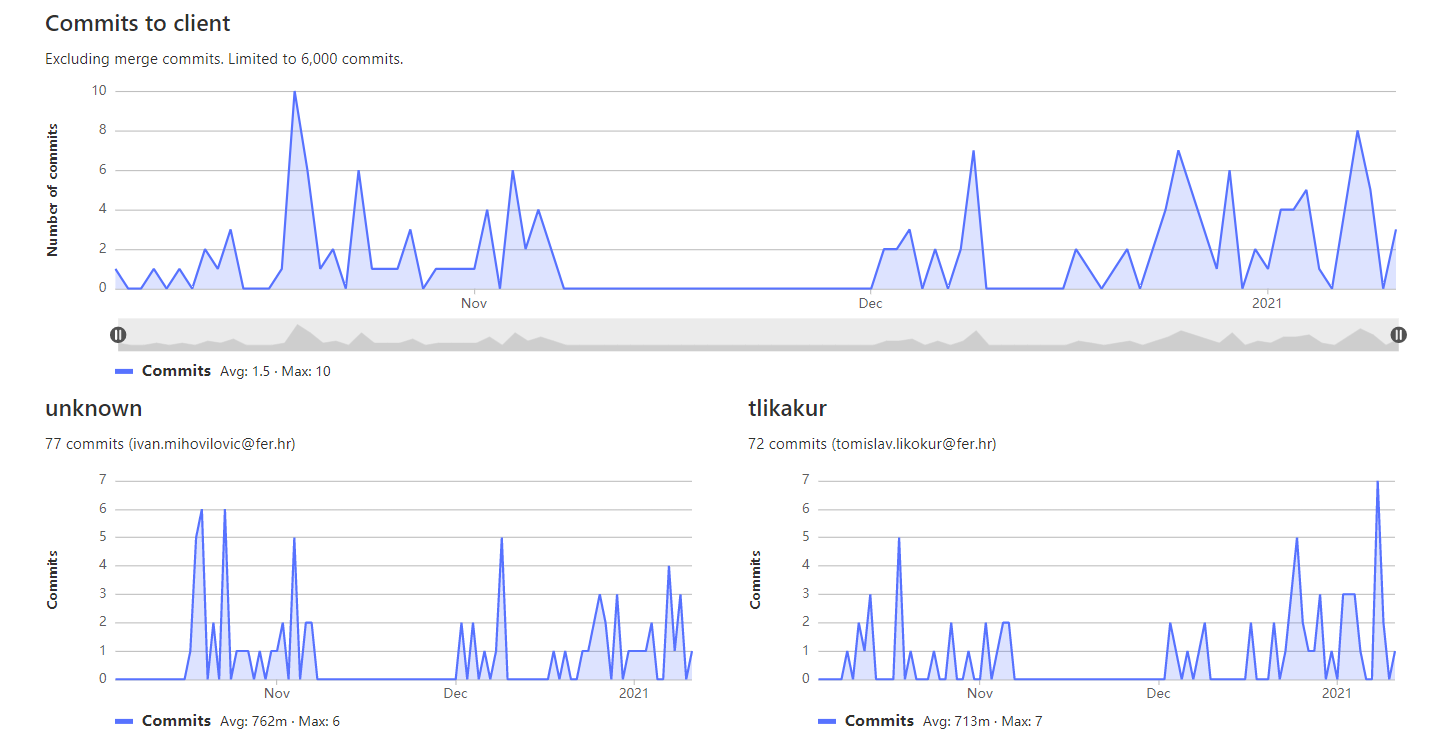
\includegraphics[scale=0.45]{slike/stat4.PNG} 
 			\centering
 			\caption{Statistika za granu client}
 			\label{fig:stat4}%label mora biti drugaciji za svaku sliku
 		\end{figure}
 	
 		 \begin{figure}[H]
 		 	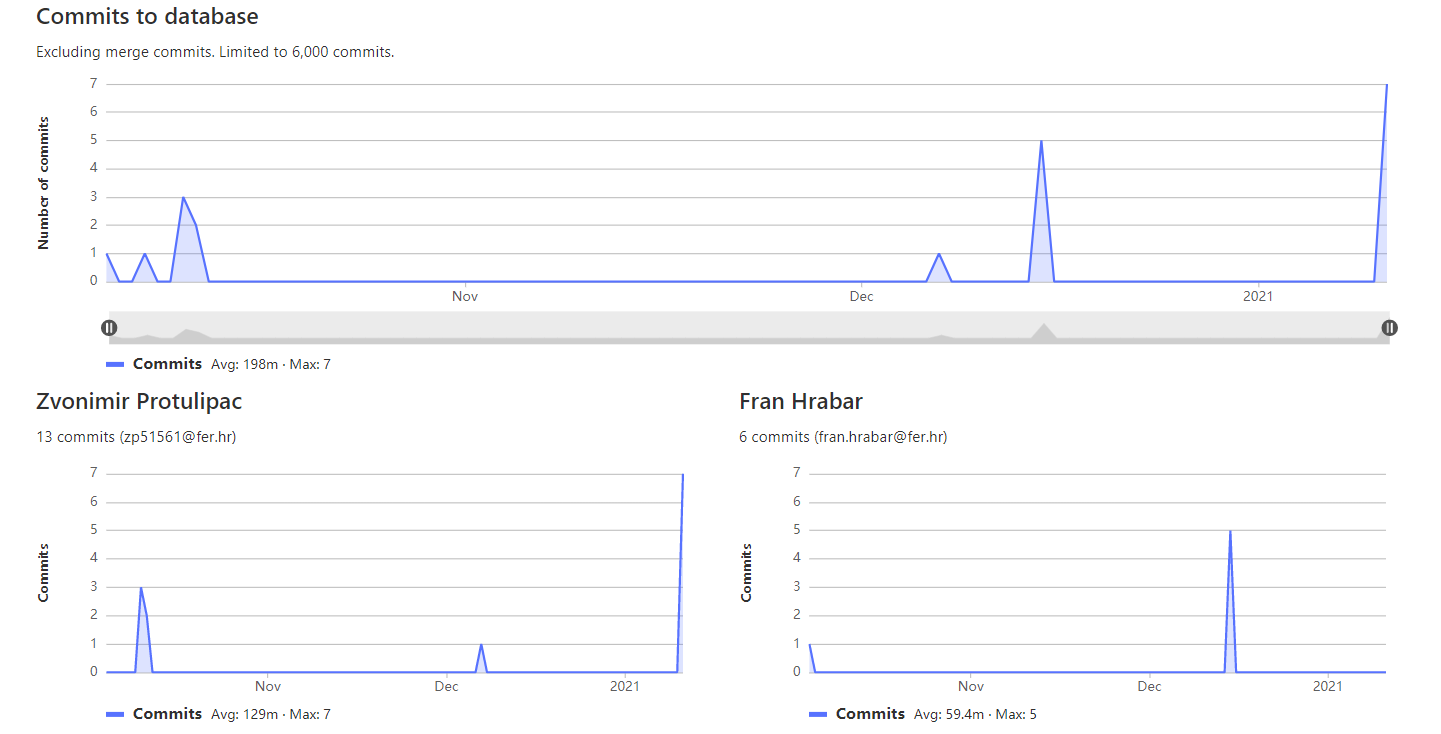
\includegraphics[scale=0.45]{slike/stat5.PNG} 
 		 	\centering
 		 	\caption{Statistika za granu database}
 		 	\label{fig:stat5}%label mora biti drugaciji za svaku sliku
 		 \end{figure}
	 
	%	\textbf{\textit{dio 2. revizije}}\\
		
		%\textit{Prenijeti dijagram pregleda promjena nad datotekama projekta. Potrebno je na kraju projekta generirane grafove s gitlaba prenijeti u ovo poglavlje dokumentacije. Dijagrami za vlastiti projekt se mogu preuzeti s gitlab.com stranice, u izborniku Repository, pritiskom na stavku Contributors.}
		
	


\end{document} %naredbe i tekst nakon ove naredbe ne ulaze u izgrađen dokument 


